% !TeX document-id = {52ccfad0-b367-4734-939e-4350e7d34ffb}
% !TeX TXS-program:compile = txs:///pdflatex/[--shell-escape]

\documentclass[
    12pt,     
    openright,
    twoside,  
    a4paper,  
    english,  
    brazil,   
    %draft
]{memoir}

\usepackage{coletanea}

\title{Programação para Web em Java}
\author{Prof. Dr. David Buzatto}
\date{v1.0 - 2021}

\makeindex


\begin{document}

\selectlanguage{portuges}
\frenchspacing 

\frontmatter

\begin{titlingpage}
    
    \newgeometry{margin=4cm}
    
    \center
    
    \noindent
    \chaptitlefont\large\textsc{Instituto Federal de Educação, Ciência e Tecnologia de São Paulo}
    \vspace{0.5cm}

    \noindent    
    \chaptitlefont\large\textsc{Câmpus São João da Boa Vista}
    \vspace{3.5cm}
    
    \noindent
    \chaptitlefont\Large\textsc{\theauthor}
    \vspace{3.5cm}
    
    \noindent
    \chaptitlefont\HUGE\textsc{\thetitle}
    \vspace*{\fill}

    \noindent
    \large\textsc{\thedate}
    
    \restoregeometry
    
\end{titlingpage}


\begin{titlingpage}
    
    \newgeometry{margin=4cm}
    
    \center
    
    \noindent
    \chaptitlefont\large\textsc{Instituto Federal de Educação, Ciência e Tecnologia de São Paulo}
    \vspace{0.5cm}
    
    \noindent    
    \chaptitlefont\large\textsc{Câmpus São João da Boa Vista}
    \vspace{2.5cm}
    
    \noindent
    \chaptitlefont\Large\textsc{\theauthor}
    \vspace{0.5cm}
    \\\chaptitlefont\large\textsc{Prof. Dr. Breno Lisi Romano}
    \\\chaptitlefont\large\textsc{Prof. Me. Everton Rafael da Silva}
    \vspace{2.5cm}
    
    \noindent
    \chaptitlefont\HUGE\textsc{\thetitle}
    \vspace{1.5cm}
    
    \hspace{.4\textwidth}
        \begin{flushright}
            \begin{minipage}{.5\textwidth}
                \SingleSpacing
                \large Programação para Web em Java.
            \end{minipage}%
        \end{flushright}
    
    \vspace*{\fill}
        
    \noindent
    \large\textsc{\thedate}
    
    \restoregeometry
    
\end{titlingpage}

\renewcommand\chaptitlefont{\normalfont\huge\bfseries\scshape\color{corAzulTema}}
    
\pdfbookmark[0]{\listfigurename}{lof}
\listoffigures*
\cleardoublepage

\pdfbookmark[0]{\listtablename}{lot}
\listoftables*
\cleardoublepage

\pdfbookmark[0]{\contentsname}{toc}
\tableofcontents*
\cleardoublepage


\mainmatter


\chapter*{Apresentação}
\epigraph{``\textit{Any fool can write code that a computer can understand. Good programmers write code that humans can understand}''.}{Martin Fowler}

\lettrine[lines=4, lhang=0.1, lraise=0, loversize=0.2, findent=0.1em]{\textcolor{corAzulTema}{P}}{rezado} aluno, seja bem-vindo! Este material contém diversos Capítulos, organizados de forma a guiá-lo no processo de fixação dos conteúdos aprendidos em aula, por meio de exercícios, desafios e de projetos práticos aplicados no contexto de desenvolvimento de aplicações Web em Java. A ordem dos Capítulos obedece a um caminho lógico que será empregado pelo professor no seu processo de aprendizagem, ou seja, a ordem dos Capítulos segue a ordem cronológica dos tópicos que serão apresentados, ensinados e treinados em laboratório.

\begin{wrapfigure}{R}{0.3\textwidth}
    \centering
    
\includegraphics[width=0.25\textwidth]{imagens/david}
\end{wrapfigure}

Antes de começar, eu gostaria de me apresentar. Meu nome é David Buzatto e sou Bacharel em Sistemas de Informação pela Fundação de Ensino Octávio Bastos (2007), Mestre em Ciência da Computação pela Universidade Federal de São Carlos (2010) e Doutor em Biotecnologia pela Universidade de Ribeirão Preto (2017). Tenho interesse em algoritmos, estruturas de dados, compiladores, linguagens de programação, algoritmos em bioinformática e desenvolvimento de jogos eletrônicos. Atualmente sou professor efetivo do Instituto Federal de Educação, Ciência e Tecnologia de São Paulo (IFSP), câmpus São João da Boa Vista. A melhor forma de contatar é através do email \textcolor{blue}{\href{mailto:davidbuzatto.ifsp@gmail.com}{davidbuzatto.ifsp@gmail.com}}.

Para que você possa aproveitar a leitura deste documento de forma plena, vale a pena entender alguns padrões que foram utilizados neste texto. As três caixas apresentadas abaixo serão empregadas para mostrar, a você leitor, respectivamente, boas práticas de programação, conteúdos complementares para melhorar e aprofundar seu aprendizado e, por fim, itens que precisam ser tratados com cuidado ou que podem acarretar em erros comuns de programação.

\begin{boaPratica}
    Essa é uma caixa de ``Boa Prática''.
\end{boaPratica}

\begin{saibaMais}
    Essa é uma caixa de ``Saiba Mais''.
\end{saibaMais}

\begin{atencao}
    Essa é uma caixa de ``Atenção''.
\end{atencao}

Você notará que este documento foi escrito de forma quase coloquial, com o objetivo de conversar com você e não com o objetivo de ser um material de pesquisa ou acadêmico. É de suma importância que você resolva cada um dos exercícios básicos de cada Capítulo, visto que a utilização de uma linguagem de programação ou tecnologia, e mais importante ainda, a obtenção de maturidade no desenvolvimento de software, é ferramenta primordial para o seu sucesso profissional e intelectual na área da Computação.

Como última observação, vale ressaltar que este documento será constantemente atualizado, sendo assim, sempre obtenha a última versão no local indicado pelo professor. Espero que este material seja útil!

\vspace*{\fill}

\FloatBarrier
\begin{figure*}[!htbp]
    \centering
    
\includegraphics[scale=0.1]{imagens/logoCC}
    \\
    Este trabalho está licenciado sob uma Licença Creative Commons Atribuição-NãoComercial-SemDerivações 4.0 Internacional. Para ver uma cópia desta licença, visite \textcolor{blue}{\url{http://creativecommons.org/licenses/by-nc-nd/4.0/}}.
\end{figure*}
\FloatBarrier

\chapter{Java para Web}\label{cap:javaParaWeb}
\epigraph{``\textit{Uma longa viagem começa com um único passo}''.}{Lao-Tsé}

\lettrine[lines=4, lhang=0.1, lraise=0, loversize=0.2, findent=0.1em]{\textcolor{corAzulTema}{N}}{ESTE} Capítulo teremos como objetivos entender o funcionamento e a arquitetura de aplicações Web desenvolvidas em Java, entender o funcionamento dos Servlets e dos JSPs e aprender a configurar e a utilizar a \textit{Integrated Development Environment} (IDE) Apache NetBeans para o apoio ao desenvolvimento de aplicações Web em Java.


\section{Introdução}

Para que você seja capaz de construir aplicações Web, primeiramente é preciso conhecer como esse serviço é estruturado. A \textit{World Wide Web} (WWW), ou simplesmente Web, é um serviço executado em diversos computadores interligados em uma rede mundial, sendo que em alguns desses computadores são executados programas chamados de \textbf{servidores}, enquanto na maioria dos outros são executados programas chamados \textbf{clientes}, que se comunicam com os servidores, estes por sua vez servem recursos para estes clientes. Na Figura~\ref{fig:cap01ClienteServidor} é ilustrado um recorte desta rede mundial.

\FloatBarrier
\begin{figure}[!htbp]
    \centering
    \caption{Recorte da estrutura da WWW}
    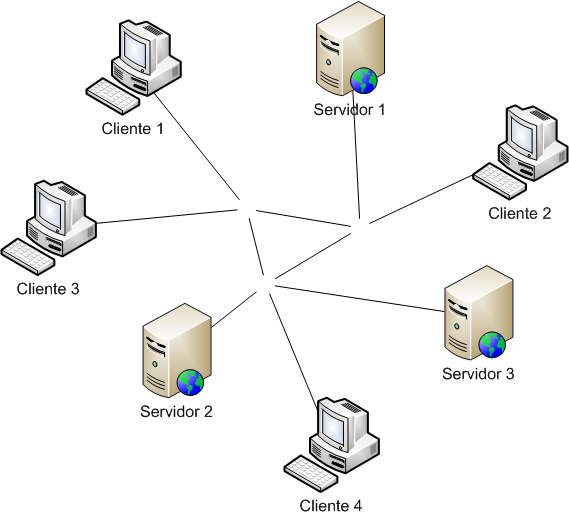
\includegraphics[scale=0.6]{imagens/cap01ClienteServidor}
    \\\textbf{Fonte:} Elaborada pelo autor
    \label{fig:cap01ClienteServidor}
\end{figure}
\FloatBarrier

Perceba que no recorte apresentado na Figura~\ref{fig:cap01ClienteServidor} são mostrados sete computadores, sendo que quatro deles atuam como clientes e os outros três como servidores. É importante entender que o que faz um computador ser cliente ou servidor é o tipo de programa que está sendo usado/executado. No nosso exemplo, as máquinas que atuam como servidores executam um programa denominado Servidor Web, que tem a capacidade de servir (disponibilizar) aos outros computadores da rede, recursos que fazem parte de uma aplicação Web, por exemplo, arquivos \textit{Hypertext Markup Language} (HTML), imagens em diversos formatos, arquivos de estilo, arquivos de \textit{script} etc. Os clientes, por sua vez, são, na maioria das vezes, os conhecidos navegadores Web, ou \textit{browsers}, que usamos no nosso dia a dia para acessar a Web e navegar em diversos \textit{sites}.

Da mesma forma que existem diversos navegadores, existem também alguns Servidores Web, sendo o Apache o mais famoso e o mais utilizado. Como já foi dito, um Servidor Web tem a função de servir recursos requisitados pelos clientes. Vamos aprender como isso funciona. Veja a Figura~\ref{fig:cap01RequestResponse}.

\FloatBarrier
\begin{figure}[!htbp]
    \centering
    \caption{Processo de requisição e resposta (\textit{request}/\textit{response})}
    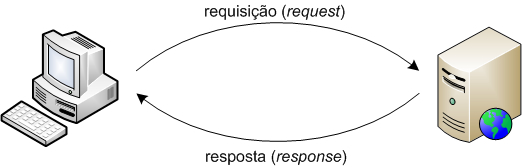
\includegraphics[scale=0.6]{imagens/cap01RequestResponse}
    \\\textbf{Fonte:} Elaborada pelo autor
    \label{fig:cap01RequestResponse}
\end{figure}
\FloatBarrier

Na Figura~\ref{fig:cap01RequestResponse} é mostrado o processo de requisição e resposta. Nesse processo, o cliente à esquerda (navegador), envia uma requisição a um recurso contido no Servidor Web (à direita) através de uma \textit{Uniform Resource Locator} (URL), sendo que nessa requisição, o cliente especifica o protocolo a ser usado, o endereço do servidor e o caminho para o recurso. Assim, uma URL tem a seguinte forma:

\begin{center}
    \textbf{\texttt{protocolo://máquina/caminho\_do\_recurso}}
\end{center}

\begin{itemize}
    
    \item Onde:
    
    \begin{itemize}
    
        \item \textbf{protocolo:} É a parte da URL que diz ao servidor qual o protocolo a ser utilizado. Quando acessamos páginas Web, por padrão, o protocolo utilizado é o \textit{Hypertext Transfer Protocol} (HTTP);
        
        \item \textbf{máquina:} É o nome ou o endereço codificado pelo \textit{Internet Protocol} (IP) da máquina que está executando o Servidor Web;
        
        \item \textbf{caminho\_do\_recurso:} É o caminho completo do recurso desejado que é disponibilizado pelo servidor.
        
    \end{itemize}
    
\end{itemize}

Confuso? Nem tanto. Vamos a um exemplo! Imagine a seguinte situação: Queremos acessar o site do IFSP. Para isso, abra o seu navegador e preencha o campo endereço com \texttt{http://www.ifsp.edu.br/} e tecle \texttt{<ENTER>}. Fazendo isso, o navegador envia uma requisição através de uma URL, usando o protocolo HTTP para a máquina \texttt{www.ifsp.edu.br}, que por sua vez retorna ao navegador uma página HTML que representa aquele endereço. 

Perceba que não especificamos o caminho do recurso! Isso não foi necessário, pois os Servidores Web são normalmente configurados para ter um comportamento padrão para responder às requisições onde só seja especificado o nome da máquina e esse comportamento padrão é direcionar para o recurso \texttt{index.html}, que é um arquivo HTML. Portanto, usar o endereço \texttt{http://www.ifsp.edu.br/} é o mesmo que usar o endereço \texttt{http://www.ifsp.edu.br/index.html}. Faça um teste! Coloque o endereço com o caminho do recurso (\texttt{index.html}) e tecle \texttt{<ENTER>}. O que aconteceu? A mesma página foi exibida não foi? Ótimo!

Vamos fazer mais um teste? Preencha novamente a barra de endereços no seu navegador com o endereço \texttt{http://j.i.uol.com.br/galerias/psp/patapon201.jpg} e tecle \texttt{<ENTER>}. Deve ter aparecido uma imagem de um jogo não foi? Vamos analisar a URL: usamos o protocolo HTTP, para pedir para o Servidor Web que está executando na máquina \texttt{j.i.uol.com.br} o recurso \texttt{patapon201.jpg}, que está armazenado no caminho \texttt{/galerias/psp/}. Este processo é ilustrado na Figura~\ref{fig:cap01ExemploRequestResponse}.

\FloatBarrier
\begin{figure}[!htbp]
    \centering
    \caption{Exemplo do processo de requisição e resposta a um recurso}
    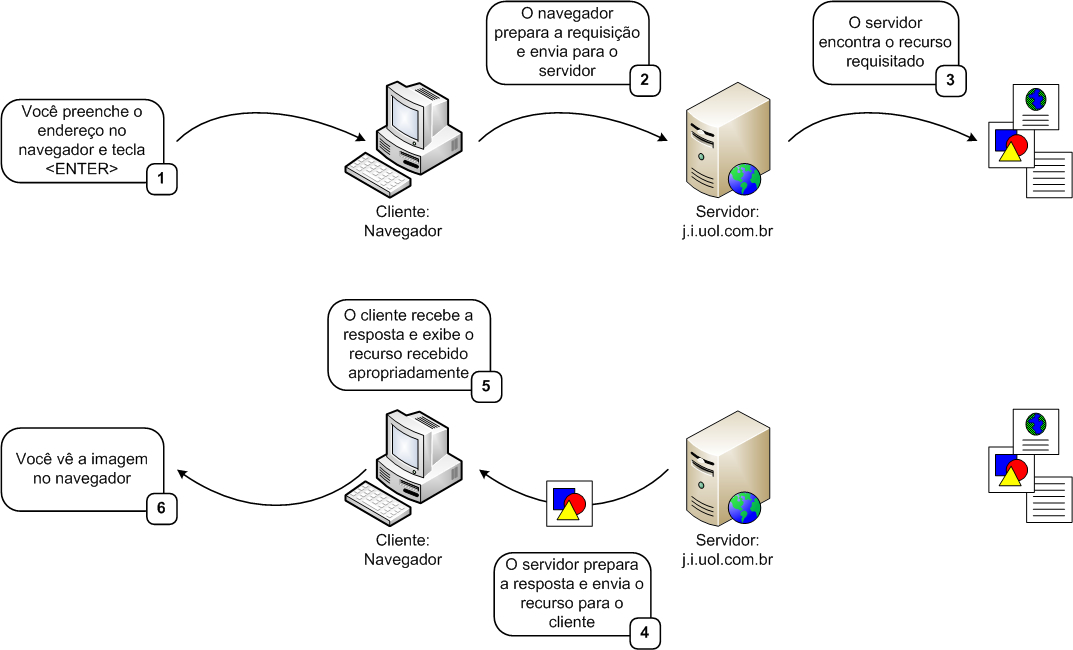
\includegraphics[scale=0.38]{imagens/cap01ExemploRequestResponse}
    \\\textbf{Fonte:} Elaborada pelo autor
    \label{fig:cap01ExemploRequestResponse}
\end{figure}
\FloatBarrier

Perceba que os passos 1, 2 e 3 da Figura~\ref{fig:cap01ExemploRequestResponse} representam o processo de requisição, enquanto os passos 4, 5 e 6 representam o processo de resposta. Note também que ao clicar em qualquer \textit{link}\footnote{O termo \textit{link} será usado para designar os \textit{hyperlinks} dos arquivos HTML} em uma página, todo esse processo é executado pelo navegador.

Muito bem! Agora que você já sabe como funciona o processo de requisição e resposta entre um navegador e um Servidor Web, podemos prosseguir com nossos estudos, agora focando em como a linguagem e a plataforma Java são utilizadas para trabalhar com aplicações Web.


\section{\textit{Container} de Servlets e Servidores de Aplicações}

Na Seção anterior você aprendeu algumas coisas novas\footnote{Provavelmente você já sabia disso!}, mas onde que a linguagem Java se encaixa nisso tudo? Quando criamos aplicações Web, além de termos páginas com código HTML e outros recursos como imagens, por exemplo, precisamos ter também componentes que processem informações que queremos que nossa aplicação manipule. Imagine que você vai fazer \textit{login} na sua rede social favorita (Facebook, Instagram etc.). Você preenche um campo com seu nome de usuário, sua senha e clica no botão para acessar o sistema e então eu lhe pergunto: O que acontece? Quem que vai validar seu usuário e sua senha? Como você deve saber uma página HTML não consegue fazer isso não é mesmo? Veja a tela de \textit{login} do Facebook na Figura~\ref{fig:cap01LoginFacebook}.

\FloatBarrier
\begin{figure}[!htbp]
    \centering
    \caption{Tela de login da rede social Facebook}
    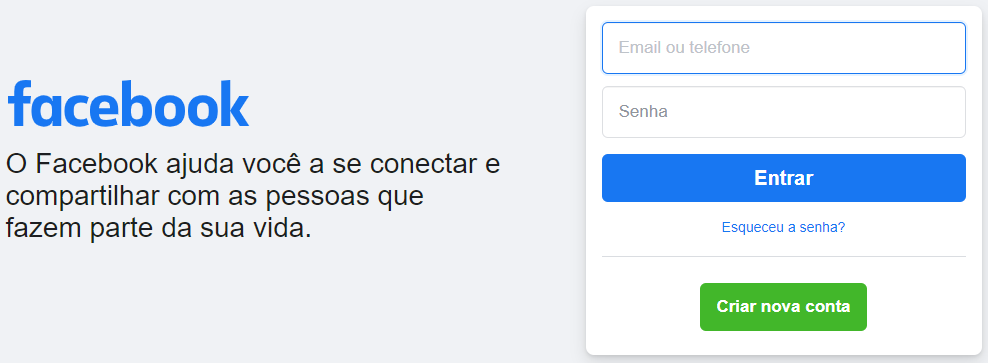
\includegraphics[scale=0.38]{imagens/cap01LoginFacebook}
    \\\textbf{Fonte:} \textit{Print screen} de \url{http://www.facebook.com}, acessado em 18/06/2021
    \label{fig:cap01LoginFacebook}
\end{figure}
\FloatBarrier

O responsável em processar os dados enviados é um componente de software que é executado no servidor em que a aplicação Web está implantada. Se a aplicação é feita em PHP, um script PHP vai fazer essa validação e retornar algum resultado com base no que foi verificado. Se a aplicação for feita em ASP.NET, Node.js etc. acontece o mesmo, ou seja, algum componente vai tratar a requisição -que enviou o usuário e a senha- e vai validá-la. Em Java é a mesma coisa!

Para que possamos utilizar código Java em nossas aplicações Web, recorremos a alguns componentes que podem ser criados dentro delas, sendo que o tipo principal desses componentes é o Servlet. Você se lembra do nosso exemplo do Facebook? Os desenvolvedores do Facebook, se usassem Java, poderiam ter criado um Servlet para receber os dados do formulário de \textit{login}, processá-los e retornar alguma resposta para o cliente, que no caso, normalmente é um navegador.

Muito bem. Sabemos então que se usarmos Java para desenvolver nossas aplicações Web, os componentes que são capazes de processar dados nas nossas aplicações e retornar resultados são os Servlets. Os Servlets são executados e gerenciados pelos \textit{Containers} de Servlets, que funcionam como um Servidor Web simples, mas com alguns ``poderes'' a mais. Esses \textit{Containers} também podem ser componentes de infraestruturas ainda mais robustas, que no caso são os Servidores de Aplicações. Um Servidor de Aplicações é como se fosse um \textit{Container} de Servlets com anabolizantes, pois além de implementar toda a especificação dos Servlets e as especificações ligadas a eles, esse tipo de servidor também implementa uma série de outras especificações da plataforma Jakarta EE (\textit{Enterprise Edition})\footnote{\url{https://jakarta.ee/}}, antigamente denominada Java EE, que fogem do propósito deste livro.

Da mesma forma que existem navegadores e Servidores Web diferentes, adivinhe só, existem também Servidores de Aplicações e \textit{Containers} de Servlets diferentes! Iremos utilizar na nossa disciplina a implementação de referência das especificações do Jakarta EE 8, que é feita pelo Servidor de Aplicações Eclipse GlassFish 5.1.0. Trabalharemos com essa versão, que mesmo não sendo a mais recente, será a ideal para o que precisaremos fazer e que tem um melhor suporte no NetBeans. Quando estamos no mundo ``Java para Web'', várias dúvidas surgem o tempo todo, visto que existe uma infinidade de termos diferentes e que normalmente causam confusão, além de existir um ecossistema absurdamente vasto. Na próxima seção vamos aprender mais alguns detalhes teóricos e na última seção vamos realizar algumas atividades!


\section{Servlets e JSPs}

Um carro serve para dirigir. Uma televisão para assistir. Uma sandália para andar. Cada um tem suas características e vão evoluindo com o tempo. Há muito tempo atrás, quando foi inventada a televisão, a imagem que era gerada não era muito boa e era em preto e branco. Foram passando os anos e a indústria foi evoluindo o equipamento. Primeiro a imagem melhorou, depois colocaram cores, depois foram criando telas cada vez maiores, mais finas, com maior resolução, inventaram outras formas de emitir imagens, gastar menos energia elétrica e assim por diante. E daí?

Tudo evolui. O que não evolui é descartado e/ou substituído. A primeira especificação dos Servlets foi lançada em 1997 e de lá para cá, a especificação foi evoluindo, permitindo que os Servlets se tornassem componentes mais versáteis e mais fáceis de utilizar. Na versão 5.1.0 do Eclipse GlassFish (perfil \textit{Web}) que implementa as especificações do Jakarta EE 8 (perfil \textit{Web}), é implementada a especificação 4.0 dos Servlets, a especificação 2.3 das JSPs (JavaServer Pages), entre outras.

Já aprendemos que os Servlets são componentes de uma aplicação Web feita em Java e que têm a capacidade de processar dados enviados a eles e gerar respostas. Um Servlet pode gerar como resposta o código HTML de uma página, entretanto essa abordagem era utilizada nas versões mais antigas dos Servlets e é totalmente desencorajada hoje em dia. Como eu disse agora a pouco, tudo evolui. Para que os desenvolvedores não precisassem mais gerar código HTML dentro do código Java de um Servlet, foram inventadas as páginas JSP. Uma página JSP é um arquivo que pode conter –e geralmente contém– código HTML e que pode interagir diretamente com algumas funcionalidades de uma aplicação Web.

A rigor, um JSP é processado pelo Servidor de Aplicações e todo o seu conteúdo é traduzido em um Servlet, que por sua vez é compilado e executado pelo Servidor. Todo esse processo é realizado nos bastidores, então não precisamos nos preocupar com esses detalhes, mas é sempre bom saber um pouquinho como as coisas funcionam não é mesmo?

Por causa desse comportamento de tradução das JSPs para Servlets, nós podemos inserir código Java dentro das JSPs, mas novamente não iremos usar essa abordagem, muito menos irei ensinar como fazer, visto que da mesma forma que gerar HTML dentro de um Servlet manualmente é desencorajado, essa abordagem de inserir código Java dentro das JSPs também não deve ser utilizada. Uma JSP deve ser usada para exibir dados, não para processá-los diretamente usando código Java. Note que não estou dizendo que não iremos manipular dados dentro das JSPs, mas sim que existem formas seguras e corretas para fazer isso. Aprenderemos esses detalhes só no Capítulo~\ref{cap:elTagLibs}, pois até lá, já teremos aprendido outros detalhes que ainda não foram apresentados.


\section{Preparação do Ambiente de Desenvolvimento}

Nesta seção você aprenderá a instalar e configurar a IDE Apache NetBeans e o Servidor de Aplicações Eclipse GlassFish 5.1 (perfil \textit{Web}).


\subsection{Apache NetBeans}

Você conhece a linguagem Java, aprendeu a teoria e a prática da programação orientada a objetos e provavelmente usou a IDE Apache NetBeans para escrever seus códigos. Neste livro trabalharemos com a versão 12 desta IDE e nos passos abaixo é explicado como deve ser feito o \textit{download} e a instalação da mesma. Esses passos podem ser pulados caso você já tenha essa versão da ferramenta instalada em seu computador. Além disso, na playlist disponível no \textit{link} \url{https://www.youtube.com/playlist?list=PLqEuQ0dDknqVcfcBHGaYrET7IBfchVS-U} você encontrará tutoriais de preparação de ambientes de desenvolvimento para trabalhar com Java para Web, que serão mantidos atualizados.

\begin{enumerate}

    \item Acesse o endereço: \url{https://www.apache.org/dyn/closer.cgi/netbeans/netbeans/12.4/Apache-NetBeans-12.4-bin-windows-x64.exe};
    
    \item Ao acessar esse \textit{link}, a versão 12.4 do Apache NetBeans será baixada;
    
    \item Baixou? Execute o instalador. As versões atuais dos instaladores NetBeans farão a instalação completa da IDE. Basta seguir o assistente, escolher o JDK instalado (8 ou superior) e aguardar o fim da instalação.
    
\end{enumerate}

Com o NetBeans instalado, abra-o. Caso o esteja executando pela primeira vez, uma página de boas-vindas será exibida. Você pode fechá-la se quiser, além de marcar para que não seja exibida novamente. Antes de criarmos o nosso primeiro projeto Java Web, precisamos baixar, instalar e configurar o Servidor de Aplicações Eclipse GlassFish.


\subsection{Eclipse GlassFish}

Como já dito, iremos instalar a versão 5.1.0 do Eclipse GlassFish, que pode ser encontrado no \textit{link} 
\url{https://www.eclipse.org/downloads/download.php?file=/GlassFish/web-5.1.0.zip}. Como não existe um instalador, faremos a instalação manualmente. Ao terminar de baixar o arquivo, descompacte-o na sua pasta de usuário do Windows. Se fez certo, vai ter algo como \texttt{C:\textbackslash Users\textbackslash <SeuUsuário>\textbackslash glassfish5\textbackslash} no seu sistema de arquivos. Pronto! O GlassFish está instalado! A última coisa que precisaremos fazer é copiar o \textit{Driver Java Database Conectivit}y (JDBC) do Sistema Gerenciador de Banco de Dados (SGBD) MariaDB/MySQL que usaremos nos próximos Capítulos deste livro.

Para isso, baixe o arquivo acessível através do \textit{link} \url{https://downloads.mariadb.com/Connectors/java/connector-java-2.7.3/mariadb-java-client-2.7.3.jar} e, ao terminar de baixar, copie-o para o diretório \texttt{C:\textbackslash Users\textbackslash SeuUsuario\textbackslash GlassFish5\textbackslash GlassFish\textbackslash\\domains\textbackslash domain1\textbackslash lib\textbackslash}.

Por fim, vamos registrar o GlassFish no NetBeans. Com o NetBeans aberto, do lado esquerdo, clique na aba \textit{Services}. Nessa aba, há um nó chamado \destaque{\textit{Servers}}. Clique com o botão direito do mouse nele e escolha \destaque{\textit{Add Server...}}. Veja a Figura~\ref{fig:cap01Servers}.

\FloatBarrier
\begin{figure}[!htbp]
    \centering
    \caption{Registrando um servidor no NetBeans}
    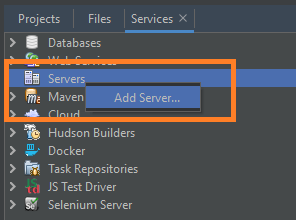
\includegraphics[scale=0.7]{imagens/cap01Servers}
    \\\textbf{Fonte:} Elaborada pelo autor
    \label{fig:cap01Servers}
\end{figure}
\FloatBarrier

Ao clicar em \destaque{\textit{Add Server...}} o assistente para registrar o servidor no NetBeans aparecerá. No primeiro passo, mostrado na Figura~\ref{fig:cap01AddServerP01}, na lista de servidores suportados, escolha \destaque{\textit{GlassFish Server}}. Na caixa de texto \destaque{\textit{Name:}} edite o nome da instância do servidor. No meu caso, adicionei a versão do mesmo, ficando ``GlassFish Server 5.1''. Ao fazer isso, clique em \destaque{\textit{Next >}}.

\FloatBarrier
\begin{figure}[!htbp]
    \centering
    \caption{Registrando um servidor no NetBeans - Passo 1}
    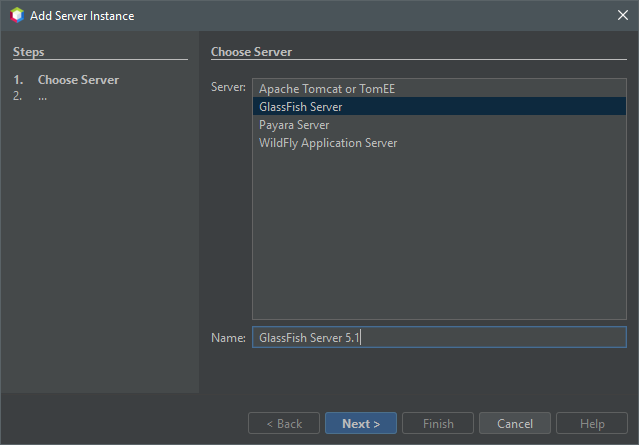
\includegraphics[scale=0.7]{imagens/cap01AddServerInstanceP01}
    \\\textbf{Fonte:} Elaborada pelo autor
    \label{fig:cap01AddServerP01}
\end{figure}
\FloatBarrier

O segundo passo do assistente precisamos definir onde os arquivos do servidor estão, como apresentado na Figura~\ref{fig:cap01AddServerP02}. Como já instalamos manualmente o servidor, não precisamos fazer o \textit{download}. Nesse passo, clique no botão \destaque{\textit{Browse...}} e procure pela instalação que fizemos há pouco. Se tudo estiver certo, a mensagem ``Detected a GlassFish...'' aparecerá logo acima dos botões dos passos do assistente. Se no seu caso estiver igual ao da Figura~\ref{fig:cap01AddServerP02}, quer dizer que está tudo certo, então basta clicar em \destaque{\textit{Next >}} para realizarmos o terceiro e último passo do assistente.

\FloatBarrier
\begin{figure}[!htbp]
    \centering
    \caption{Registrando um servidor no NetBeans - Passo 2}
    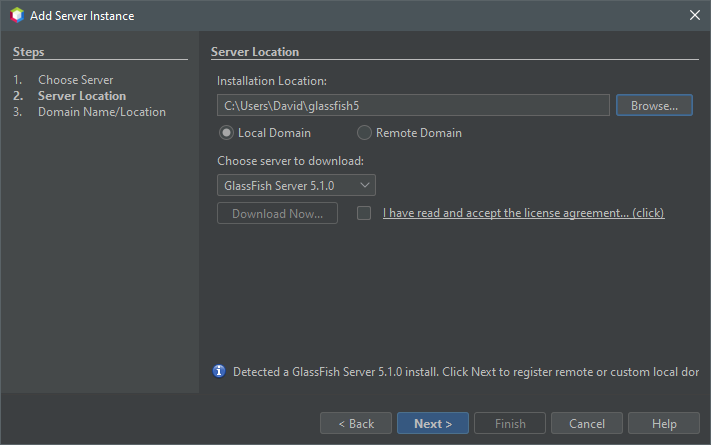
\includegraphics[scale=0.7]{imagens/cap01AddServerInstanceP02}
    \\\textbf{Fonte:} Elaborada pelo autor
    \label{fig:cap01AddServerP02}
\end{figure}
\FloatBarrier

Nesse passo, faremos a última configuração necessária, que consiste apenas em definir o nome do usuário administrador do servidor. Na Figura~\ref{fig:cap01AddServerP03} isso pode ser visto na caixa de texto \destaque{\textit{User Name:}} que está preenchida com ``admin''. Ao preencher o nome de usuário, clique em \destaque{\textit{Finish}}.

\FloatBarrier
\begin{figure}[!htbp]
    \centering
    \caption{Registrando um servidor no NetBeans - Passo 3}
    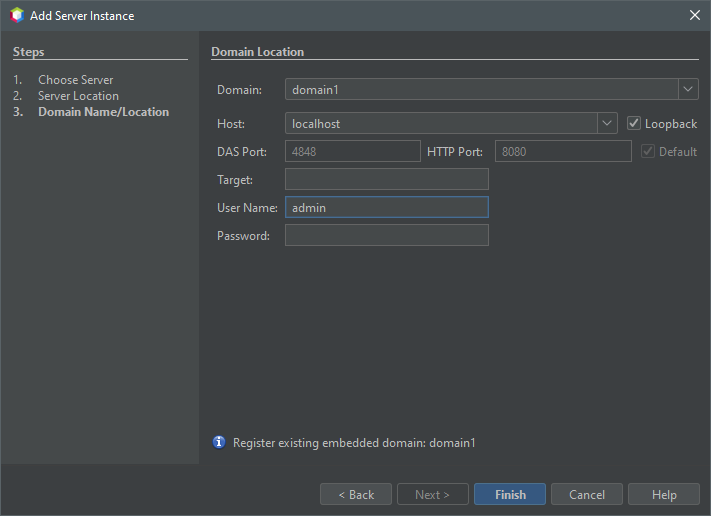
\includegraphics[scale=0.7]{imagens/cap01AddServerInstanceP03}
    \\\textbf{Fonte:} Elaborada pelo autor
    \label{fig:cap01AddServerP03}
\end{figure}
\FloatBarrier

Ao fazer isso, o GlassFish estará pronto para ser utilizado. Caso haja alguma dúvida, visite o \textit{link} mencionado que contém uma playlist de tutoriais para a configuração de ambientes de desenvolvimento.


\subsection{Primeiro Projeto Java para Web}\label{subsec:primeiroProjeto}

Agora que temos tudo configurado, iremos criar nosso primeiro projeto Java para Web! Siga os passos abaixo:

\begin{itemize}

    \item \textbf{Passo 1:} Clique no menu \destaque{\textit{File}} e depois em  \destaque{\textit{New Project...}}. Fazendo isso, o assistente para criação de projetos será aberto. Na lista de categorias, expanda o item  \destaque{\textit{Java with Ant}} e escolha  \destaque{\textit{Java Web}}. Na lista de tipos de projeto, escolha  \destaque{\textit{Web Application}} e clique no botão  \destaque{\textit{Next >}};
    
    \item \textbf{Passo 2:} Preencha o campo \destaque{\textit{Project Name:}} com ``OlaMundoWeb'' (sem acentos, sem as aspas e tudo junto). Em \destaque{\textit{Project Location:}}, defina o diretório onde o projeto será salvo. Deixe a opção \destaque{\textit{Use Dedicated Folder for Storing }} marcada e clique no botão \destaque{\textit{Next >}};
    
    \item \textbf{Passo 3:} Na opção \destaque{\textit{Server:}} escolha o ``GlassFish Server 5.1'', ou a opção com o nome que você definiu ao registrar o GlassFish. Em \destaque{\textit{Java EE Version:}} escolha ``Jakarta EE 8 Web''. Em \destaque{\textit{Context Path:}} deixe o valor padrão (/OlaMundoWeb), que é o mesmo nome que demos ao nosso projeto. Clique em \destaque{\textit{Next >}};
    
    \item \textbf{Passo 4:} No último passo, o assistente perguntará quais \textit{frameworks} nós queremos inserir no nosso projeto. Nós não vamos usar nenhum, então basta clicar em \destaque{\textit{Finish}}. Fazendo isso, o novo projeto será criado e será aberto no NetBeans, sendo que por padrão será criado um arquivo HTML (\texttt{index.html}) que será a página inicial da nossa aplicação.
    
\end{itemize}

\begin{saibaMais}
    Existem diversas definições para \textit{framework}, sendo que, informalmente, podemos definí-los como um conjunto de classes que incorporam uma abstração que tem como objetivo de solucionar problemas de um tipo ou domínio específico.
\end{saibaMais}

Muito bem, criamos nosso primeiro projeto. Vamos executá-lo para ver o que acontece? Na barra de ferramentas do NetBeans tem um botão com uma seta verde, igual a um botão de ``\textit{play}'' de um reprodutor de mídias. Quando você clicar nesse botão, você vai ver que várias mensagens começarão a aparecer na janela de saída do NetBeans. Essas mensagens irão mostrar para nós o que está acontecendo no momento, como a inicialização do GlassFish (caso não esteja iniciado) etc. O que está esperando? Clique lá no ``\textit{play}''. Assim que tudo estiver pronto, será aberta uma janela do seu navegador, onde será mostrado o conteúdo do \texttt{index.html}, que no nosso caso será uma página com ``TODO write content'' escrito.

Muito bem! Temos nossa primeira aplicação rodando no GlassFish! Fácil não é mesmo? Por enquanto não vamos nos preocupar com a estrutura do projeto, iremos aprender os detalhes aos poucos. Vamos colocar um pouco de código HTML no nosso \texttt{index.html}? Ele deve estar aberto no NetBeans. Se não estiver, procure o arquivo \texttt{index.html} na pasta \destaque{\textit{Web Pages}} do seu projeto e clique duas vezes no arquivo para abri-lo no editor. Vamos mudar o título, escrevendo ``Meu Primeiro Projeto Java para Web'' no lugar de ``TODO supply a title'' e dentro da \textit{tag} \inlineHTMLCode{<body>} do arquivo, inserir um \textit{heading} \inlineHTMLCode{<h1>} e um parágrafo com um \textit{link} para o site do IFSP. Veja na Listagem~\thechapter.\ref{listagem:projetos/capitulo01/OlaMundoWeb/web/index.html} como deve ficar seu código.

\htmlCode{Arquivo \texttt{index.html}}{projetos/capitulo01/OlaMundoWeb/web/index.html}

Salve o arquivo depois de editá-lo. Se o navegador ainda estiver aberto no \texttt{index.html}, volte a ele e aperte a tecla \texttt{<F5>} do seu teclado para mandar o navegador atualizar a página. Se não estiver, dê o ``\textit{play}'' no projeto de novo. Você vai ver que a página vai exibir as alterações que fizemos. Teste o \textit{link} para ver se está funcionando. A página deve ter ficado como mostrada na Figura~\ref{fig:cap01OlaMundoIndex}.

\FloatBarrier
\begin{figure}[!htbp]
    \centering
    \caption{Arquivo \texttt{index.html} em exibição}
    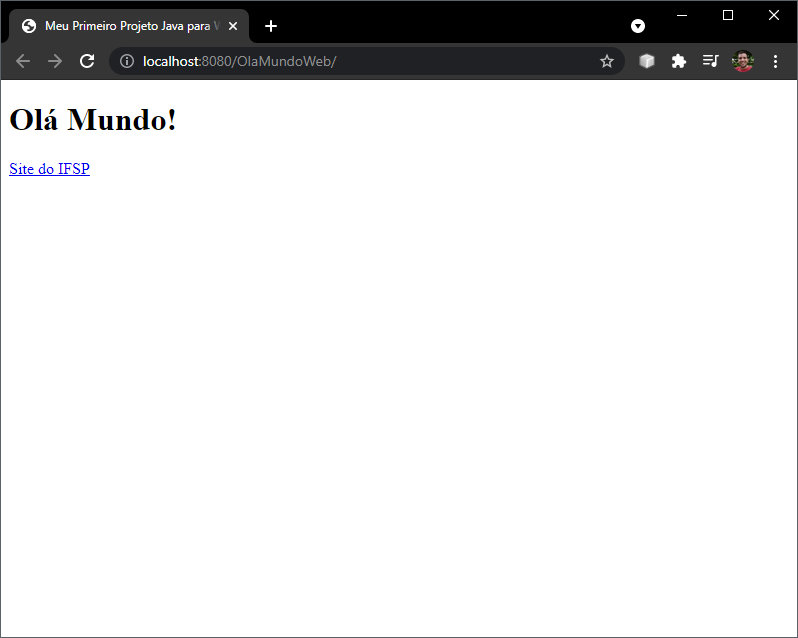
\includegraphics[scale=0.7]{imagens/cap01OlaMundoIndex}
    \\\textbf{Fonte:} Elaborada pelo autor
    \label{fig:cap01OlaMundoIndex}
\end{figure}
\FloatBarrier

Poderíamos ter usado um arquivo \textit{JavaServer Pages} (JSP) ao invés de usar um arquivo HTML, permitindo a existência de outros tipos de estruturas que vamos aprender no decorrer da disciplina, mas por enquanto vamos manter o HTML. Vamos testar os Servlets agora? Como primeiro exemplo, nós vamos criar um Servlet manualmente, enquanto os outros que vamos desenvolver durante o nosso curso serão feitos usando um assistente do NetBeans, mas essa forma fácil nós só vamos aprender a partir do Capítulo~\ref{cap:processamentoFormularios}.

Aprenderemos como criar manualmente um Servlet, para que possamos aprender alguns detalhes importantes sobre o funcionamento de aplicações Web feitas em Java. Antes disso, e daqui por diante, sempre que você criar um projeto Web, antes de qualquer coisa, siga os seguintes passos para adicionar a biblioteca necessária para viablizar o desenvolvimento.

\begin{itemize}
    
    \item \textbf{Passo 1:} Na árvore do projeto, clique com o botão direito do mouse em \destaque{\textit{Libraries}} e clique no item \destaque{\textit{Add Library...}}. Veja a Figura~\ref{fig:cap01AddLibraryProjeto};
    
    \FloatBarrier
    \begin{figure}[!htbp]
        \centering
        \caption{Inserção de bibliotecas no projeto}
        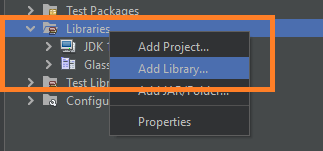
\includegraphics[scale=0.9]{imagens/cap01AddLibraryProjeto}
        \\\textbf{Fonte:} Elaborada pelo autor
        \label{fig:cap01AddLibraryProjeto}
    \end{figure}
    \FloatBarrier
    
    \item \textbf{Passo 2:} Ao fazer isso, o diálogo \destaque{\textit{Add Library}} será exibido assim como apresentado na Figura~\ref{fig:cap01AddLibraryDialog}. Clique no botão \destaque{\textit{Import...}};
    
    \FloatBarrier
    \begin{figure}[!htbp]
        \centering
        \caption{Diálogo de inserção de bibliotecas}
        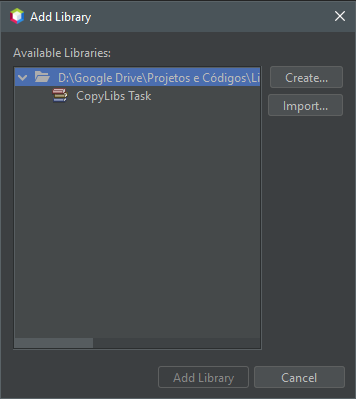
\includegraphics[scale=0.9]{imagens/cap01AddLibraryDialog}
        \\\textbf{Fonte:} Elaborada pelo autor
        \label{fig:cap01AddLibraryDialog}
    \end{figure}
    \FloatBarrier
    
    \item \textbf{Passo 3:} Outro diálogo, intitulado \destaque{\textit{Import Library}}, aparecerá. Nesse diálogo, mostrado na Figura~\ref{fig:cap01AddLibraryImport}, escolha a biblioteca \destaque{\textit{Jakarta EE Web 8 API Library}} e clique no botão \destaque{\textit{Import Library}};
    
    \FloatBarrier
    \begin{figure}[!htbp]
        \centering
        \caption{Diálogo de importação de bibliotecas}
        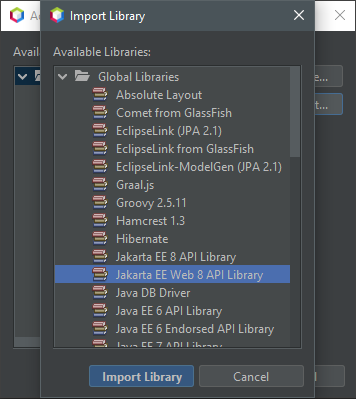
\includegraphics[scale=0.9]{imagens/cap01AddLibraryImport}
        \\\textbf{Fonte:} Elaborada pelo autor
        \label{fig:cap01AddLibraryImport}
    \end{figure}
    \FloatBarrier
    
    \item \textbf{Passo 4:} Ao fazer isso, a biblioteca será importada no projeto, ou seja, uma cópia dela será feita para dentro da sua estrutura. Note que na Figura~\ref{fig:cap01AddLibraryImported} é mostrado novamente o diálogo \destaque{\textit{Add Library}}, mas agora a biblioteca importada está disponível para ser inserida no projeto. Para isso, selecione a bibliteca e clique no botão \destaque{\textit{Add Library}};
    
    \FloatBarrier
    \begin{figure}[!htbp]
        \centering
        \caption{Diálogo de inserção de bibliotecas com biblioteca importada}
        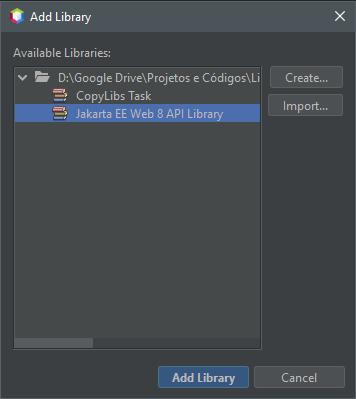
\includegraphics[scale=0.9]{imagens/cap01AddLibraryImported}
        \\\textbf{Fonte:} Elaborada pelo autor
        \label{fig:cap01AddLibraryImported}
    \end{figure}
    \FloatBarrier
    
    \item \textbf{Passo 5:} Por fim, você perceberá que a biblioteca agora faz parte das bibliotecas do projeto, podendo ser usada. Veja a Figura~\ref{fig:cap01AddLibraryFinished}.
    
    \FloatBarrier
    \begin{figure}[!htbp]
        \centering
        \caption{Biblioteca inserida no projeto}
        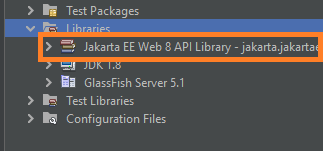
\includegraphics[scale=0.9]{imagens/cap01AddLibraryFinished}
        \\\textbf{Fonte:} Elaborada pelo autor
        \label{fig:cap01AddLibraryFinished}
    \end{figure}
    \FloatBarrier
    
\end{itemize}

Agora que importamos e inserimos a biblioteca \destaque{\textit{Jakarta EE Web 8 API Library}} no nosso projeto, podemos usar as funcionalidades Web implementadas pelo Jakarta EE. Nos próximos passos criaremos e testaremos nosso primeiro Servlet.

\begin{itemize}
    
    \item \textbf{Passo 1:} Na árvore que representa a estrutura do projeto, procure pela pasta \destaque{\textit{Source Packages}} e expanda-a (clique no sinal de ``+'' à esquerda). Dentro dela haverá um pacote com o ícone cinza chamado \destaque{\textit{<default package>}}. Como vocês devem saber, é desencorajado que se trabalhe com pacotes padrão em Java, então vamos criar um pacote. Clique com o botão direito na pasta \destaque{\textit{Source Packages}} e escolha \destaque{\textit{New}}, procure pela opção \destaque{\textit{Java Package...}} e clique nela. Se esta opção não estiver sendo exibida, clique na opção \destaque{\textit{Other...}} (no final da lista), escolha \destaque{\textit{Source Packages}} nas categorias, e \destaque{\textit{Java `Package}} nos tipos de arquivos e clique em \destaque{\textit{Next >}}. Preencha o campo \destaque{\textit{Package Name:}} com ``olamundoweb'' (sem as aspas) e clique em \destaque{\textit{Finish}}. O pacote será criado;
        
    \item \textbf{Passo 2:} Repita o Passo 1, só que agora clicando com o botão direito no pacote que você criou e crie um pacote chamado ``servlets'' (sem as aspas). O nome do pacote deverá ser preenchido com ``olamundoweb.servlets''. Seu projeto agora terá um pacote chamado ``olamundoweb.servlets''. O resultado desses dois primeiros passos podem ser vistos na Figura~\ref{fig:cap01CriacaoPacote};
    
    \FloatBarrier
    \begin{figure}[!htbp]
        \centering
        \caption{Criação do pacote \texttt{olamundoweb.servlets}}
        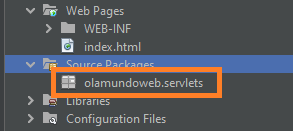
\includegraphics[scale=0.9]{imagens/cap01CriacaoPacote}
        \\\textbf{Fonte:} Elaborada pelo autor
        \label{fig:cap01CriacaoPacote}
    \end{figure}
    \FloatBarrier
            
    \item \textbf{Passo 3:} Clique com o botão direito no pacote  \destaque{\texttt{olamundoweb.servlets}}, escolha \destaque{\textit{New}} e clique na opção \destaque{\textit{Java Class...}}. Novamente, se não a encontrar, clique em \destaque{\textit{Other...}} e procure por \destaque{\textit{Java Class...}} (está na categoria ``Java'') e clique em \destaque{\textit{Next >}}. Preencha o campo \destaque{\textit{Class Name:}} com ``OlaServlet'' (sem as aspas) e clique em \destaque{\textit{Finish}}. A classe será criada dentro do pacote especificado e será aberta no editor. Você vai ter algo como apresentado na Listagem~\thechapter.\ref{listagem:projetos/capitulo01/parciais/OlaServlet.java} (sem os comentários);
    
    \javaCode{olamundoweb/servlets/OlaMundoWeb.java}{projetos/capitulo01/parciais/OlaServlet.java}
    
    \item \textbf{Passo 4:} Para que uma classe seja um Servlet, precisamos estender a classe \texttt{HttpServlet}, que está contida no pacote \texttt{javax.servlet.http}\footnote{O Jakarta EE 8 segue a nomenclatura antiga do Java EE, onde o pacote base é o \texttt{javax}. A partir da versão 9, esse pacote foi renomeado para \texttt{jakarta}.} e então implementar os métodos HTTP que queremos que nosso Servlet trate. Não se preocupe, ainda vamos aprender sobre os métodos HTTP, então o mais importante a saber, por enquanto, é que os métodos HTTP mais usados são o \texttt{GET} (\inlineJavaCode{doGet(...)} de \texttt{HttpServlet}) e o  \texttt{POST} (\inlineJavaCode{doPost(...)} de  \texttt{HttpServlet}). Então teremos que sobrescrever cada um desses métodos e ainda criaremos um terceiro que será invocado a partir dos outros dois. Confuso? Vamos ver como o código ficaria. Leia os comentários e copie o código da Listagem~\thechapter.\ref{listagem:projetos/capitulo01/OlaMundoWeb/src/java/olamundoweb/servlets/OlaServlet.java} para o seu editor.
    
\end{itemize}

\FloatBarrier
\javaCode{olamundoweb/servlets/OlaMundoWeb.java}{projetos/capitulo01/OlaMundoWeb/src/java/olamundoweb/servlets/OlaServlet.java}
\FloatBarrier
    
Até agora criamos uma classe chamada \texttt{OlaServlet}, que estende a classe \texttt{HttpServlet}. Sobrescrevemos os métodos \inlineJavaCode{doGet(...)} e \inlineJavaCode{doPost(...)} herdados de \texttt{HttpServlet} que tratam respectivamente os métodos \texttt{GET} e \texttt{POST} do protocolo HTTP e criamos um terceiro método, chamado \inlineJavaCode{processRequest(...)}, que tem a mesma assinatura dos métodos \inlineJavaCode{doGet(...)} e \inlineJavaCode{doPost(...)} e que é invocado dentro deles. É no \texttt{processRequest} que iremos colocar o código que queremos executar, sendo que no nosso exemplo, estamos mandando imprimir na saída duas Strings: ``Olá Mundo!'' e ``Meu Primeiro Servlet!''. Ou seja, se chamarmos o Servlet usando o método \texttt{GET}, o método \inlineJavaCode{doGet(...)} será invocado e passará o controle para o método \inlineJavaCode{processRequest(...)} que irá imprimir as mensagens na saída. O mesmo acontece para o método \texttt{POST}.

Muito bem, você tem um Servlet totalmente funcional, mas ai você se pergunta: ``Como vou chamar esse Servlet através do navegador?''. Então eu respondo: no código completo, você percebeu que há uma anotação chamada \inlineJavaCode{@WebServlet}? É essa anotação que vai fornecer essa informação\footnote{Antigamente precisávamos fazer o mapemanto em um arquivo \textit{Extensible Markup Language} (XML) (\url{http://pt.wikipedia.org/wiki/XML}) chamado de Descritor de Implantação (DI, em inglês \textit{Deployment Descriptor}), representado pelo arquivo \texttt{web.xml}, o que atualmente, com as versõs mais novas do Jakarta/Java EE, não é mais necessário para algumas situações.}, expecificamente no parâmetro \texttt{urlPatterns}. Perceba que configuramos esse parâmetro com um array de Strings com um elemento: ``/ola''. Com isso, podemos agora acessar o \texttt{OlaServlet} a partir de uma URL, que no nosso caso é ``\url{http://localhost:8080/OlaMundoWeb/ola}'', ou seja, usamos o protocolo HTTP, para a máquina \texttt{localhost} (que é o endereço da nossa máquina), na porta 8080 (que é a porta que o GlassFish ouve por padrão), para acessar a aplicação chamada \texttt{OlaMundoWeb} (isso vem do contexto que criamos no Passo 3 da Subseção~\ref{subsec:primeiroProjeto}, volte lá para dar uma olhadinha), para por fim acessar o recurso mapeado sob o nome de ``ola'' que no caso é o nosso Servlet. 

Sei que pode parecer um pouco confuso no começo, mas logo você vai pegar o jeito da coisa. Dê um ``play'' no projeto de novo. O navegador vai abrir no endereço da aplicação novamente. Insira o ``ola'' (sem as aspas) no final da URL e tecle \texttt{<ENTER>}. O que aconteceu? Apareceu uma página em branco não foi? É claro, afinal, nosso Servlet não gera HTML, mas apenas imprime duas mensagens na saída padrão não é mesmo? Mas como podemos ver essas mensagens? Volte no NetBeans e procure, logo abaixo, uma aba chamada \destaque{\textit{Output}}. Ela provavelmente vai estar selecionada. Dentro dela devem haver outras três abas: \destaque{\textit{OlaMundoWeb (run)}} que deve estar selecionada e que é usada para mostrar o processo de construção do projeto da nossa aplicação, \destaque{\textit{Java DB Database Process}}, que exibe o \textit{status} do Java DB e, por fim, \destaque{\textit{GlassFish Server 5.1}}, que exibe a saída padrão do GlassFish. Clique nessa última aba e veja o que está escrito lá embaixo: as duas mensagens que enviamos para a saída padrão através do método \inlineJavaCode{System.out.println(...)} dentro do Servlet, sendo que o fim de cada linha conterá os caracteres \texttt{|\#]}\footnote{Esse sufixo é inserido automaticamente pelo servidor.}! Veja o resultado na Figura~\ref{fig:cap01SaidaGlassFish}. Volte ao navegador e tecle \texttt{<ENTER>} novamente no endereço do Servlet. Volte no NetBeans. Mais duas mensagens! Fácil não é mesmo?

\FloatBarrier
\begin{figure}[!htbp]
    \centering
    \caption{Saída do GlassFish 5.1}
    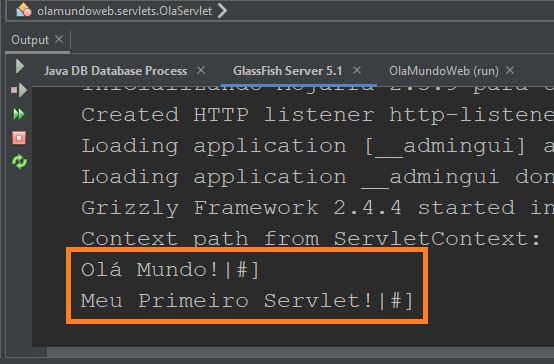
\includegraphics[scale=0.9]{imagens/cap01SaidaGlassFish}
    \\\textbf{Fonte:} Elaborada pelo autor
    \label{fig:cap01SaidaGlassFish}
\end{figure}
\FloatBarrier
    
Por mais que nosso exemplo não tenha nenhuma utilidade aparente, ele foi importante para nós entendermos o funcionamento básico de uma aplicação Web feita em Java. Nos próximos Capítulos vamos colocar o que aprendemos em prática, além de aprender várias outras coisas com o objetivo criarmos um sistema de cadastro na forma de uma aplicação Web. Não se esqueça de praticar o que aprendemos até agora. 


\section{Resumo}

Neste Capítulo aprendemos o que é e como funciona uma aplicação Web em Java. Aprendemos a criar nosso primeiro projeto e alguns detalhes sobre a tecnologia que estamos utilizando. Executamos nossa aplicação e fizemos algumas modificações nela para vermos o que estava sendo feito. Criamos também –de forma manual– um Servlet, que como aprendemos é um dos componentes principais de uma aplicação Web em Java.


\section{Exercícios}

\begin{exercicioSemArquivo}{}{}{}
    O que é um Servidor Web?
\end{exercicioSemArquivo}

\begin{exercicioSemArquivo}{}{}{}
    Como são chamados os clientes que utilizamos para acessar aplicações servidas por um Servidor Web? Cite alguns exemplos.
\end{exercicioSemArquivo}

\begin{exercicioSemArquivo}{}{}{}
    Diferencie um Servidor Web de um Container de Servlets.
\end{exercicioSemArquivo}


\section{Projetos}

\begin{projetoSemArquivo}{}{}{}
    Crie um novo projeto Java Web no NetBeans, com o nome de ``MinhaPagina'', edite o \texttt{index.html} de modo a exibir seus dados pessoais, seus interesses etc. Tente inserir uma imagem também. Dica: a imagem deve estar dentro do projeto do NetBeans. Pense se você entende o motivo pelo qual o arquivo \texttt{index.html} é mostrado por padrão quando você acessa sua página através da URL \url{HTTP://localhost:8080/MinhaPagina}.
\end{projetoSemArquivo}

\begin{projetoSemArquivo}{}{}{}
    Crie um novo projeto Java Web no NetBeans, com o nome de ``Contador''. Nesse projeto você deve criar um Servlet manualmente e dentro do método \inlineJavaCode{processRequest(...)} use uma estrutura de repetição para direcionar para a saída padrão os números de 1 a 30.
\end{projetoSemArquivo}

\begin{projetoSemArquivo}{}{}{}
    Crie um novo projeto Java Web no NetBeans, com o nome de ``Fibonacci''. Nesse projeto, você deve criar um Servlet manualmente e dentro do método \inlineJavaCode{processRequest(...)} use uma estrutura de repetição para exibir os 30 primeiros termos da série de Fibonacci. Crie um método chamado \texttt{fibonacci} dentro do seu Servlet, sendo que este método deve receber como parâmetro um inteiro e retornar um inteiro. O inteiro que é recebido como parâmetro é o número do termo desejado, enquanto o inteiro que é retornado é o termo correspondente ao parâmetro que foi recebido. A série de Fibonacci é formada inicialmente pelos números 1 e 1, sendo que os próximos números da série são gerados a partir da soma dos dois números anteriores. Os sete primeiros termos da série de Fibonacci são $1, 1, 2, 3, 5, 8, 13$, onde: $2 = 1 + 1, 3 = 1 + 2, 5 = 2 + 3, 8 = 3 + 5, 13 = 5 + 8$.
    
    Exemplos de chamadas da função fibonacci:
    \begin{itemize}
        \item \texttt{fibonacci(2)}: retorna 1
        \item \texttt{fibonacci(5)}: retorna 5
        \item \texttt{fibonacci(7)}: retorna 13
    \end{itemize}
    
\end{projetoSemArquivo}
\chapter{Processamento de Formulários}
\epigraph{``\textit{O modo como você reúne, administra e usa a informação determina se vencerá ou perderá.}''.}{Bill Gates}

\lettrine[lines=4, lhang=0.1, lraise=0, loversize=0.2, findent=0.1em]{\textcolor{corAzulTema}{N}}{ESTE} Capítulo teremos como objetivos entender o funcionamento de formulários HTML e conseguirmos diferenciar os métodos do protocolo HTTP e como tratá-los.


\section{Introdução}

Neste Capítulo vamos começar a aprender a criar algo útil! No Capítulo anterior, aprendemos as bases do desenvolvimento Web em Java, criamos alguns programas de brinquedo\footnote{Programa de brinquedo é todo programa criado para apresentar algum conceito e que, normalmente, não tem uma utilidade prática além da pedagógica.} para aplicar as técnicas que aprendemos e agora vamos aprender mais alguns detalhes, mas dessa vez nossos programas serão mais elaborados. Vamos começar?


\section{Formulários}

A forma tradicional de se desenvolver aplicações para Web que interajam com o servidor é utilizando os chamados formulários. Um formulário é composto normalmente por um conjunto de componentes que permitem que o usuário forneça dados para serem submetidos ao servidor. Quando esses dados são recebidos pelo servidor, algum componente da aplicação vai tratá-los, sendo que no nosso caso, esse componente vai ser implementado na forma de um Servlet.
Atualmente existem diversas técnicas para a criação de aplicações Web, sendo que, dependendo da técnica/tecnologia, a forma de submeter dados ao servidor é diferente. Uma dessas técnicas é o chamado Asynchronous JavaScript and XML (AJAX) que hoje em dia é implementado de inúmeras formas. Neste livro não iremos aprender a usar AJAX, porque infelizmente não teremos tempo, mas garanto que se você se empenhar no decorrer do nosso curso, ao final, você estará apto a aprender a trabalhar com AJAX.

Abra o NetBeans e crie um novo projeto Java Web. Dê o nome de ``PrimeiroFormulario'' (sem as aspas). Sempre que for criar um novo projeto, siga os passos descritos na Subseção \label{subsec:primeiroProjeto} do Capítulo 1. Com o projeto criado, vamos editar o \texttt{index.html}. Nele vamos alterar o título da página e criar nosso primeiro formulário, que será usado para preenchermos dados pessoais de um cliente. Veja na Listagem~\thechapter.\ref{listagem:projetos/capitulo02/PrimeiroFormulario/web/index.html} como ficou o código. Não se esqueça de copiá-lo no seu \texttt{index.html}.

\htmlCode{Protótipo do formulário de dados do cliente (\texttt{index.html})}{projetos/capitulo02/PrimeiroFormulario/web/index.html}

Copiou? Salve o arquivo e execute a aplicação. Você vai ter algo como o mostrado na Figura~\ref{fig:cap02PrimeiroFormulario}.

\FloatBarrier
\begin{figure}[!htbp]
    \centering
    \caption{Visualização do protótipo do formulário de dados do cliente}
    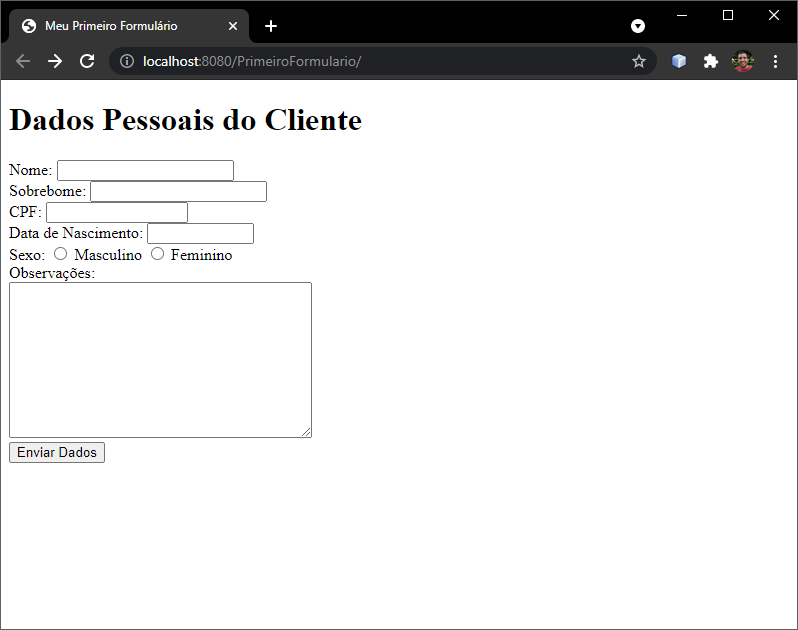
\includegraphics[scale=0.7]{imagens/cap02PrimeiroFormulario}
    \\\textbf{Fonte:} Elaborada pelo autor
    \label{fig:cap02PrimeiroFormulario}
\end{figure}
\FloatBarrier

Quanta coisa! O formulário não ficou uma obra prima, mas esse não é nosso objetivo agora. Precisamos entender o que cada \textit{tag} faz. Vamos agora analisar o código da Listagem~\thechapter.\ref{listagem:projetos/capitulo02/PrimeiroFormulario/web/index.html} e entender o protótipo que fizemos. Irei detalhar apenas as \textit{tags} \texttt{<form>} e seus componentes, pois acredito que você já conheça as outras que foram utilizadas. Vamos lá então:

\begin{itemize}
    \item \textbf{Linha 13:} Nesta linha abrimos a \textit{tag} \texttt{<form>} que delimita um formulário HTML. Note que fechamos a \textit{tag} form na linha 43. Todas as \textit{tags} que forem inseridas entre \texttt{<form>} e \texttt{</form>} farão parte do formulário;
    
    \item \textbf{Linha 15:} Criamos um \textit{label} (tag <label>) com o conteúdo ``Nome: ''. A \textit{tag} \texttt{<label>} é usada para criar um rótulo. Ao invés de usar a \textit{tag} \texttt{<label>}, poderíamos simplesmente ter inserido o texto que queremos mostrar no formulário, mas como o texto que estamos utilizando tem o propósito de ser um rótulo para um campo do formulário, iremos utilizar essa tag para deixar nosso código mais organizado e inserir uma certa carga semântica no nosso código;
    
    \item \textbf{Linha 16:} Criamos um \textit{input} (campo de entrada) do tipo \textit{text} (texto) com tamanho de 20 colunas e com o nome de ``nome''. Dentre as \textit{tags} que representam componentes nos formulários, a \texttt{<input>} é uma delas. Existem vários tipos de \textit{inputs}, diferenciados pela propriedade \texttt{type}, e que vamos aprender aos poucos. A propriedade \texttt{size}, como você deve ter percebido, é utilizada para configurar a largura do campo de texto. A propriedade \texttt{name} é utilizada pelo navegador para identificar os dados do componente em questão no momento de enviar os dados para o servidor. Não entendeu a utilidade da propriedade \texttt{name}? Não se preocupe, logo vai fazer sentido;
    
    \item \textbf{Linha 17:} Usamos a \textit{tag} \texttt{<br/>} para pular uma linha;
    
    \item \textbf{Linhas 19 a 29:} Os próximos três campos (sobrenome, CPF e data de nascimento) são bem parecidos com o primeiro;
    
    \item \textbf{Linha 32:} Criamos um input do tipo \textit{radio} (botão de rádio), com nome configurado como ``sexo'' e com o valor (\texttt{value}) configurado com ``M'';
    
    \item \textbf{Linha 33:} Idem à linha anterior, com a diferença que o valor é ``F''. Note que a propriedade name de ambos os radios é a mesma, pois eles representam o mesmo campo (sexo). Perceba que no navegador, se você selecionar um deles e depois clicar no outro, o que estava selecionado previamente deixa de ser selecionado. Se a propriedade \texttt{name} for diferente, eles serão considerados campos diferentes e então esse comportamento da seleção não existirá. Note ainda que você pode ``amarrar'' quantos radios você precisar;
    
    \item \textbf{Linha 38:} Nessa linha definimos uma área de texto. Esse componente, representado pela \textit{tag} textarea é utilizado, como o próprio nome já diz, para criar uma área de texto livre, onde o usuário poderá digitar uma quantidade arbitrária de texto. Note que para utilizar um textarea nós precisamos usar a \textit{tag} de fechamento (<textarea>), ao invés de fazer da forma que estamos fazendo com os inputs. A novidade nesse componente são as propriedades cols e rows, que são usadas respectivamente para definir a quantidade de colunas e de linhas do componente;
    
    \item \textbf{Linha 41:} Por fim, nessa linha definimos um input do tipo submit, que é um botão que tem o comportamento padrão de, ao ser clicado, submeter (enviar) os dados do formulário para o servidor. Note que usamos a propriedade value para definir o texto do botão.
\end{itemize}

Agora que já conhecemos alguns dos componentes que podemos utilizar nos nossos formulários, mas você deve estar se perguntando: ``Tudo bem, o input do tipo submit é usado para enviar os dados do formulário para o servidor, mas onde eu digo ao submit para onde os dados do formulário devem ser enviados?''. Vamos à resposta!
Eu tenho dito várias vezes que o componente que vai tratar os dados de um formulário na nossa aplicação é o Servlet não é mesmo? Então precisamos criar um Servlet que vai receber esses dados e então configurar o formulário para direcionar os dados inseridos nele para o Servlet apropriado.
Vamos criar o Servlet? Mas agora iremos fazer de uma forma mais automática do que a que estamos fazendo desde que aprendemos a trabalhar com os Servlets. Na pasta de pacotes de código-fonte do projeto, crie um pacote chamado ``primeiroformulario.servlets'' (sem as aspas). Clique com o botão direito no pacote criado, escolha ``Novo'' e procure pela opção ``Servlet...''. Se não encontrou, escolha a propriedade ``Outro...'', selecione ``Web'' na categoria, ``Servlet'' no tipo de arquivo e clique em ``Próximo''. 
Preencha o campo ``Nome da classe'' com ``ProcessaDadosClienteServlet'' (sem as aspas) e clique em ``Próximo''. Nesse passo, note que o assistente nos pede o nome do Servlet e o padrão de URL. Lembra que criávamos nossa classe do Servlet e implementávamos seu esqueleto, além de fazer seu mapeamento no DI, manualmente? Agora o NetBeans vai fazer tudo isso para nós automaticamente! Deixe o campo ``Nome do Servlet'' com o valor padrão (que é o nome da classe) e preencha o campo ``Padrão(ões) de URL'' com ``/processaDadosCliente'' (sem as aspas). Não iremos aprender sobre os padrões de inicialização na nossa disciplina, mas nada impede que você aprenda para que eles servem, basta consultar a bibliografia recomendada nas referências bibliográficas da apostila tudo bem? Tudo feito? Clique em ``Finalizar''.
Ao fazer isso, o nosso Servlet será criado e aberto no editor. Como eu sei que você é uma pessoa super curiosa, dê uma olhada no web.xml para ver que o Servlet que foi criado já foi mapeado lá! Legal hein?
Note que o NetBeans já implementou o esqueleto do Servlet para nós. O primeiro método implementado é o processRequest. Lembra-se dele? É nele que vamos inserir o código que queremos que o Servlet execute. Após o fechamento do bloco deste método, note que existe uma linha onde está escrito ``HttpServlet methods. Click on the + sign on the left to Edit the code.''. Siga a sugestão da frase e clique no ``+''. O que apareceu? A implementação dos métodos GET e POST, sendo que dentro delas é chamado o processRequest! Viu só? Da mesma forma que fazíamos manualmente! Não iremos mexer ali, então você pode contrair novamente esta seção do código clicando no sinal de ``–''.
Note que além de implementar o esqueleto do nosso Servlet, o NetBeans também inseriu um trecho de código dentro do processRequest. O código que está inserido configura o tipo de retorno do Servlet (response.setContentType(...)), obtém o canal de escrita do Servlet, escreve uma série de Strings que representam uma página HTML nesse canal e o fecha. Você se lembra que já falei algumas vezes que não iremos implementar Servlets que geram código HTML? Então, vamos limpar esse método, tirando todo o código que foi inserido dentro dele. Vá no editor e apague o conteúdo entre as linhas 30 (response.setContentType(...)) e 45 (``\}''), incluindo elas. Seu processRequest deve estar vazio agora.
Antes de codificarmos, vamos a mais um pouquinho de teoria. Você se lembra, lá no comecinho da primeira aula, que eu falei que o cliente manda uma requisição para o servidor e ele manda uma resposta? Nos Servlets, essa requisição e essa resposta são representadas respectivamente por objetos do tipo HttpServletRequest e HttpServletResponse. Note que os três métodos implementados nos nossos Servlets (processRequest, doGet e doPost) recebem dois parâmetros, sendo eles dos tipos que mencionei. Qual a conclusão que você chega então? Os dados enviados pelo cliente ao servidor estão dentro do objeto do tipo HttpServletRequest, que chamamos de request no nosso código e os dados que enviamos de volta ao cliente devem ser inseridos no objeto do tipo HttpServletResponse, que demos o nome de response.
Sabendo disso, agora ficou fácil! Os dados do formulário de clientes que estamos construindo serão recebidos pelo nosso Servlet através do objeto apontado por request! Legal não é? Mas ainda falta um detalhe... Não informamos ao formulário para quem ele deve enviar os dados! Vamos fazer isso agora. Volte no index.jsp e procure pela \textit{tag} form (a mesma que está na linha 15 da Listagem 2.1). Para informarmos à \textit{tag} form qual é o destino dos seus dados, utilizamos a propriedade action, sendo que nesta propriedade, colocamos a URL do componente que deve tratar os dados do formulário. Mapeamos nosso Servlet usando o padrão ``/processaDadosCliente'' não foi? Então, qual será a URL do nosso Servlet? Resposta: ``http://localhost:8084/PrimeiroFormulario/processaDadosCliente''. Vamos editar nossa \textit{tag} form então, configurando a propriedade action para a URL citada. Na Listagem 2.2 você pode ver como ficou o código da \textit{tag} form. Note que não estou listando todo o arquivo.

Listagem 2.2: Configurando a propriedade action da \textit{tag} form
 
Fonte: do autor
Isso que dizer que, quando clicarmos no botão ``Enviar Dados'' (que é um input do tipo submit), os dados que estiverem preenchidos nos componentes que estão dentro deste formulário, serão enviados para http://localhost:8084/PrimeiroFormulario/processaDadosCliente, que é o endereço do nosso Servlet! Já alterou o arquivo? Salvou? Legal! Atualize a página, preencha os campos e clique no botão ``Enviar Dados''. O que aconteceu? Uma página em branco foi exibida não é? E na barra de endereços, o que apareceu? O endereço do Servlet mais um monte de ``coisas''! Os detalhes sobre isso nós iremos aprender na próxima seção, então não se preocupe por enquanto.
Você se lembra dos nossos primeiros exemplos? Acessávamos o endereço do Servlet, uma página em branco era exibida e duas Strings eram direcionadas para a saída do Tomcat, lembra? Quem fazia esse direcionamento era o Servlet não era? Vamos fazer a mesma coisa com o nosso Servlet de dados dos clientes, mas mostraremos os dados que foram preenchidos nos formulários. Vamos lá então?
Volte ao Servlet, vamos implementar o método processRequest. Qual é mesmo o nome do parâmetro do método processRequest que armazena os dados enviados pelo cliente? É o request certo? Veja o código da Listagem 2.3. Leia o comentário que fiz.













Listagem 2.3: Implementação do método processRequest
 
Fonte: do autor
Copiou o código? Legal. Vamos entender o que está acontecendo. Na linha 14 é declarada uma variável do tipo String com o nome de ``nome''. Essa variável é inicializada com o valor obtido ao se chamar o método getParameter( String param ) de request. O parâmetro passado ao método getParameter, que é uma String, é o nome que foi dado ao componente do formulário, que no caso foi ``nome''. Estude as linhas 15, 16, 17, 18 e 19 e tente fazer um paralelo com o formulário contido no index.jsp. Note que a String que é passada como parâmetro no método getParameter(...) sempre reflete o nome dado ao componente do formulário através da propriedade name. Veja a linha 17. Declaramos uma variável chamada dataNascimento que é inicializada com o valor do parâmetro ``dataNasc'' (configurado no formulário).
O que fizemos até a linha 19 foi criar uma variável que vai receber o valor de cada componente do formulário. A partir da linha 21, até o final do método, direcionamos para a saída os dados que foram obtidos. Vamos testar? Salve o Servlet e execute o projeto (botão de ``play'', lembra?). Na página, preencha o formulário, clique em ``Enviar Dados'' e volte no NetBeans para ver o que aconteceu. Olhe na janela de saída! Lá estão os dados que você preencheu no formulário! Muito bem! Imagine agora se esse fosse um sistema real. Esses dados recebidos dentro do Servlet poderiam alimentar uma query SQL para inserir esse cliente em um banco de dados! Legal não é?! A partir desse ponto, você já deve estar entendendo melhor o que está acontecendo não é mesmo? Mas e aquele monte de coisas escritas no endereço do navegador depois de clicar em Enviar Dados? Esse comportamento está intrinsecamente ligado ao tipo de método HTTP que estamos usando. Vamos para a próxima seção, vou explicar isso lá.


\section{Métodos HTTP}

O protocolo HTTP 1.1, que usamos em nossas aplicações Web, define uma série de métodos que podem ser usados para tratar diversos tipos de requisições. Na nossa vida, como desenvolvedores Web, iremos nos importar somente com os métodos GET e POST. Sendo assim vamos detalhá-los.
<Saiba mais:
Quer conhecer os outros métodos HTTP (HEAD, TRACE, etc.)? Acesse este link: http://www.w3.org/Protocols/rfc2616/rfc2616-sec9.html (em inglês)
>


\subsection{Método GET}

O método GET (to get = obter) é usado principalmente para pedir ao servidor algum recurso. Quando nós fazemos uma pesquisa no Google, por exemplo, estamos usando o método GET. Qualquer URL que colocamos na barra de endereço do nosso navegador é enviada ao servidor usando o método GET. Vamos fazer um teste. Entre na página do Google (www.google.com.br) e pesquise por ``métodos http'' (sem as aspas). Ao clicar em pesquisar, o resultado será mostrado no navegador. Veja a barra de endereços. Haverá algo assim:
%\url{http://www.google.com.br/#hl=pt-BR\&biw=1440\&bih=713\&q=métodos+http\&aq=f\&
%aqi=g10\&aql=\&oq=\&gs_rfai=\&fp=90f65ad7da748e6d}
Parece grego, mas não é! Vamos entender a URL. Estamos usando o protocolo HTTP, para acessar a máquina www.google.com.br. O recurso é representado pelo restante da URL:
%hl=pt-BR\&biw=1440\&bih=713\&q=métodos+http\&aq=f\&aqi=g10\&aql=\&oq=\&gs_rfai=\&
fp=90f65ad7da748e6d
Vamos dividir esse resto da URL nos símbolos ``\&''. Vamos obter isso aqui:
hl=pt-BR
biw=1440
bih=713
q=métodos+http
aq=f
aqi=g10
...
Note que a forma de cada pedaço da parte correspondente ao recurso é x=y, onde ``x'' é o nome de uma variável e ``y'' é o valor. No nosso exemplo, a variável ``q'' tem o valor ``métodos+http'' que no caso é a nossa consulta! Ou seja, o componente que trata as pesquisas do Google, entende que a variável ``q'' vai conter o valor da pesquisa que estamos fazendo!
Execute novamente o nosso projeto, limpe todos os campos e preencha o campo ``Nome'' com ``Juca'' (sem as aspas) e o campo ``Sexo'' com Masculino e clique em ``Enviar Dados''. Veja a URL que foi obtida na barra de endereços:
%T\url{http://localhost:8084/PrimeiroFormulario/processaDadosCliente?nome=Juca&
%sobrenome=&cpf=&dataNasc=&sexo=M&observacoes=}
Veja o caminho do recurso!
%processaDadosCliente?nome=Juca\&sobrenome=\&cpf=\&dataNasc=\&sexo=M\&observacoes=
O que isso quer dizer:
Senhor ``processaDadosCliente'', por favor, receba as variáveis nome, sobrenome, cpf, dataNasc, sexo e observacoes, utilize seus valores e me devolva o recurso associado a eles. O ponto de interrogação após o mapeamento do Servlet (/processaDadosCliente) indica que o que vem depois dele (do ponto de interrogação) são variáveis HTTP. Cada variável, como já vimos, está na forma x=y, onde ``x'' é a variável e ``y'' é o valor, sendo que elas são separadas por ``\&''. Então temos: ``nome'' igual a ``Juca'', ``sobrenome'' igual a vazio, ``cpf'' igual a vazio, ``dataNasc'' igual a vazio, ``sexo'' igual a ``M'' e ``observacoes'' igual a vazio. A saída no NetBeans deve ter ficado assim:
Dados do Cliente:
Nome: Juca
Sobrenome: 
CPF: 
Data de Nascimento: 
Sexo: Masculino
Observações:
Vamos mandar a requisição novamente para o NetBeans, só que agora modificando a URL ao invés de usar o formulário. Dê o sobrenome de ``Santos'' ao Juca e defina o CPF como 123456789. Preencheu a URL na barra de endereços? Tecle <ENTER> e veja o que aconteceu no NetBeans. A saída deve ter sido essa aqui:
Dados do Cliente:
Nome: Juca
Sobrenome: Santos
CPF: 123456789
Data de Nascimento: 
Sexo: Masculino
Observações:
Então, basicamente, ao usarmos o método GET, indicamos que queremos algum recurso do servidor. Quando enviamos dados através do método GET, esses dados, na forma de variáveis, são codificados na própria URL. O nosso formulário do index.jsp utiliza por padrão o método GET. Qualquer formulário usa por padrão o método GET. Se quisermos mudar o método de envio do formulário, precisamos usar a propriedade method da \textit{tag} form. Ai você me pergunta: Porque usaríamos outro método? O GET já não funciona? E eu respondo: Sim, o GET funciona, mas imagine a seguinte situação: você vai armazenar os dados de um usuário de um sistema. Você vai mandar vários dados para o servidor, inclusive uma senha. O que acontece? A senha enviada vai aparecer na URL! Afinal, a senha é um campo do formulário! O ideal seria ninguém a ver correto? Outro problema. O tamanho de uma URL é fixo! Então não podemos mandar conteúdos de tamanho arbitrário, visto que iremos perder dados caso usemos o método GET! Então como fazemos? Método POST, ao resgate!
<Saiba mais:
O tamanho fixo das URLs é uma restrição imposta pelos navegadores e/ou pelos servidores, visto que o protocolo HTTP não fixa o tamanho de uma URL. Mais detalhes aqui: http://www.boutell.com/newfaq/misc/urllength.html (em inglês)
>



\subsection{Método POST}

O método POST (to post = postar) é usado para enviar dados ao servidor. Ao contrário do método GET, ao usar o método POST, as variáveis de um formulário não são inseridas na URL, mas sim no corpo da requisição. Sendo assim, a quantidade dos dados enviados usando o método POST pode ter qualquer tamanho, desde apenas uma variável, até arquivos de tamanhos variados. Você já enviou uma foto para o Orkut não enviou? Saiba que ela foi enviada usando o método POST.
Como eu já disse na seção anterior, por padrão, o navegador envia os dados de um formulário usando o método GET. Caso queiramos mudar esse comportamento, basta usar a propriedade method da \textit{tag} form. Vamos fazer isso? Vá ao NetBeans, abra o arquivo index.jsp caso não esteja aberto, procure pela \textit{tag} form e insira a propriedade method. Veja na Listagem 2.4 como deve ficar:
Listagem 2.4: Usando o método POST para enviar a requisição para o Servlet
 
Fonte: do autor
Salve o arquivo e execute o projeto novamente. Preencha o formulário e clique em ``Enviar Dados''. Verifique a URL, pois agora as variáveis não serão mais codificadas nela. Verifique a saída no NetBeans para constatar que os dados continuam a ser enviados. Edite novamente o index.jsp e mude o método para GET. Teste novamente. As variáveis devem estar aparecendo novamente na URL não é? De novo, edite o index.jsp e volte para o método POST e teste de novo.
Muito bem! Estamos quase acabando. Tenho certeza que você deve estar entendendo tudo. Se não estiver, releia o que está com dúvida tudo bem? Vamos à nossa última seção, que vai tratar de mais um pouquinho de teoria.



\subsection{Tratando Métodos HTTP}

Você deve lembrar que quando criamos um Servlet manualmente, nós criávamos três métodos, o processRequest(...), o doGet(...) e o doPost(...). Quando criamos um Servlet usando o assistente do NetBeans, ele também cria uma estrutura parecida com a que a gente criava manualmente, além de já realizar o mapeamento do nosso Servlet. Na seção anterior falamos dos métodos GET e POST do protocolo HTTP, que são os que nós usamos como desenvolvedores Web. Você já deve ter notado, e eu também já falei, que um Servlet deve implementar o método HTTP que ele deve tratar. A implementação de um método HTTP em um Servlet deve ser feita dentro de métodos que por padrão são nomeados ``doXXX(...)'', onde XXX deve ser trocado pelo nome do método HTTP em questão. Sendo assim, requisições usando o método GET são tratadas dentro do método doGet(...) do Servlet. Requisições usando o método POST são tratadas dentro do método doPost(...) do Servlet e assim por diante.
Note então que todos os Servlets que criamos até agora se comportam da mesma forma tanto para o método GET quanto para o método POST, pois sempre que a requisição chega no Servlet, o método apropriado é escolhido, entretanto, tanto o método doGet(...), quanto o método doPost(...), direcionam o fluxo de execução para o método processRequest(...)! Nós sempre iremos fazer assim, pois é muito mais prático e não precisamos ficar nos preocupando qual método um Servlet trata, precisamos apenas nos preocupar em modificar a propriedade method da \textit{tag} form quando quisermos mudar o método que deve ser utilizado. 
Muito legal não é mesmo? Com isso fechamos nossa segunda semana. Na próxima aula, iremos aprender a trabalhar com dois recursos superimportantes da especificação das JSPs: EL (Expression Language) e TagLibs. Após aprender essas duas funcionalidades, estaremos prontos para começar a criar nosso primeiro projeto que trabalha com banco de dados, mas antes disso ainda iremos formalizar e aprender algumas coisinhas. Ah, não se esqueça de praticar o que aprendemos até agora! Vamos ao resumo da semana.


\section{Resumo}

Nesta aula demos um passo muito importante para a nossa vida como desenvolvedores Web, pois aprendemos a trabalhar com formulários e entendemos o funcionamento dos métodos GET e POST que fazem parte do protocolo HTTP. Como você já deve ter percebido, os formulários desempenham um papel importantíssimo nas aplicações Web. Tenho certeza que de agora em diante, sempre que você usar uma aplicação Web, você saberá como aquele formulário funciona. Para colocar em prática o que aprendemos, criamos um projeto Java Web no NetBeans e fizemos diversos testes.

\section{Exercícios}

1 – Qual a diferença entre os métodos GET e POST? Quando devemos utilizar um ou o outro?

\section{Projetos}

2 – Incremente o projeto que criamos durante a aula inserindo mais alguns campos no formulário: email, logradouro, número, complemento, cidade, estado, CEP, se o cliente tem ou não filhos. Utilize apropriadamente os tipos de input que aprendemos até agora.
3 – Crie um novo projeto Java Web, com o nome de ``FormularioDVD'' (sem as aspas), que deve ter um formulário usado para enviar dados de um DVD. Um DVD, no nosso caso, deve ter: número, título, ator/atriz principal, ator/atriz coadjuvante, diretor/diretora e ano de lançamento. Para tratar o formulário, crie um Servlet usando o assistente do NetBeans. Esse Servlet deve obter os dados enviados através do formulário e imprimi-los na saída padrão (usando System.out.println(...)), como foi feito no exemplo construído durante esta aula. Esse formulário deve usar o método POST.
4 – Crie um novo projeto Java Web, com o nome de ``FormularioProduto'' (sem as aspas), que deve ter um formulário usado para enviar dados de um Produto. Um Produto, no nosso caso, deve ter: código de barras, descrição, unidade de medida (unidade ou kg), quantidade por embalagem, fabricante (nome). Para tratar o formulário, crie um Servlet usando o assistente do NetBeans. Esse Servlet deve obter os dados enviados através do formulário e imprimi-los na saída padrão (usando System.out.println(...)), como foi feito no exemplo construído durante esta aula. Esse formulário deve usar o método POST.
5 – Crie um novo projeto Java Web, com o nome de ``CalculadoraWeb'' (sem as aspas), que deve ter um formulário usado para atuar como uma calculadora. Nesse formulário, deve haver dois campos (``número 1'' e ``número 2'') e um conjunto de radios para representar a operação a ser realizada (adição, subtração, multiplicação e divisão). Para tratar o formulário, crie um Servlet usando o assistente do NetBeans. Esse Servlet deve obter os dados enviados através do formulário, executar a operação escolhida pelo usuário e imprimir o resultado na saída padrão (usando System.out.println(...)), como foi feito no exemplo construído durante esta aula. Esse formulário deve usar o método GET. Faça testes de envio dos dados usando apenas a URL gerada depois da primeira submissão.
6 – Crie um novo projeto Java Web, com o nome de ``TamanhoString'' (sem as aspas), que deve ter um formulário com apenas um campo usado para enviar uma String de qualquer tamanho para um Servlet. Utilize uma textarea para o usuário poder inserir essa String no formulário. O Servlet deve obter a String enviada e imprimir o a quantidade de caracteres da String na saída padrão (usando System.out.println(...)), como foi feito no exemplo construído durante esta aula. Qual método HTTP deve ser utilizado nessa situação? Justifique sua resposta.
7 – Desafio – Crie um novo projeto Java Web, com o nome de ``EhPrimo'' (sem as aspas), que deve ter um formulário usado para enviar um número inteiro para um Servlet, que por sua vez deve verificar se este número é primo. O resultado do teste deve ser impresso na saída padrão. Esse formulário deve usar o método GET.
8 – Desafio – Crie um novo projeto Java Web, com o nome de ``EquacaoSegundoGrau'' (sem as aspas), que deve ter um formulário usado para enviar os coeficientes de uma equação de segundo grau para um Servlet, que por sua vez deve calcular as raízes da equação em questão e imprimir essas raízes na saída padrão. As raízes de uma equação do segundo grau podem ser determinadas usando a fórmula de Bhaskara (http://pessoal.sercomtel.com.br/matematica/fundam/eq2g/eq2g.htm, http://pt.wikipedia.org/wiki/Bhaskara\_II). O Servlet deve verificar também se os coeficientes passados representam uma equação do segundo grau válida. Esse formulário deve usar o método GET.
\chapter{\textit{Expression Language} e \textit{TagLibs}}
\epigraph{``\textit{A magia da linguagem é o mais perigoso dos encantos}''.}{Edward Bulwer-Lytton}

\lettrine[lines=4, lhang=0.1, lraise=0, loversize=0.2, findent=0.1em]{\textcolor{corAzulTema}{N}}{ESTE} Capítulo teremos como objetivo entender a sintaxe, o propósito e como utilizar tanto a \textit{Expression Language} quanto as \textit{tags} JSP, além de aprendermos a lidar com as \textit{tags} disponibilizadas na \textit{Java Standard Template Library} (JSTL).


\section{Introdução}

Nesta aula iremos aprender duas funcionalidades muito importantes e úteis do mundo Java Web: a \textit{Expression Language} (EL) e as TagLibs. Essas duas funcionalidades nos ajudarão na tarefa de não misturar código Java nas nossas JSPs. Você se lembra quando falei que era possível inserir código Java dentro das JSPs, não lembra? Falei também que isso não deveria ser feito, pois deixa o código difícil de ler e de manter, além de fazer com que o trabalho do Web designer (que normalmente conhece mais HTML e CSS) se torne difícil, visto que ele teria que ter um bom conhecimento em Java e em como as JSPs funcionam. Usando a EL e as TagLibs, a manipulação de dados, provenientes dos Servlets, se torna muito mais fácil, pois utiliza uma sintaxe simples e fácil de entender, ajudando no trabalho de quem não conhece muito bem o funcionamento de aplicações Web em Java. Vamos começar?


\section{\textit{Expression Language} (EL)}

A EL é um recurso da especificação das JSPs que permite utilizarmos uma sintaxe especial para obter dados que gostaríamos de mostrar nas nossas páginas, além de permitir que façamos algumas outras coisas, como por exemplo, avaliar uma expressão lógica. Como de costume, iremos utilizar um projeto para aprendermos o recurso que estamos estudando. Crie um projeto Java Web com o nome ``UsandoELeTagLibs'' (sem as aspas). Nesse projeto teremos um formulário no \texttt{index.html} que terá seus dados tratados por um Servlet, que por sua vez irá fazer algum processamento e direcionar o resultado gerado para uma páina JSP, chamada \texttt{exibeDados.jsp}.

Edite o \texttt{index.html} e insira um formulário. O meu ficou como mostrado na Listagem~\thechapter.\ref{listagem:projetos/capitulo03/UsandoELeTagLibs/web/index.html}. Copie o código para o seu \texttt{index.html} e teste. 

\htmlCode{Formulário para envio de dados de um produto (\texttt{index.html})}{projetos/capitulo03/UsandoELeTagLibs/web/index.html}

Note que nesse arquivo temos algumas coisas novas. A primeira novidade é a \textit{tag} \texttt{<style>} na linha 10. Usamos essa \textit{tag} para criar regras de estilo para formatar/estilizar a visualização do nosso nosso documento. Tudo que usarmos de formatação como alinhamento, cor de texto etc., será definido usando estilos. Esses estilos são codificados usando as folhas de estilo \textit{Cascading Style Sheets} (CSS). A sintaxe é muito simples. As definições em CSS são chamadas de seletores. Sendo assim, a definição \texttt{.alinharDireita} (linha 11) indica que estamos definindo um seletor que é uma classe de formatação (denotada pelo ponto (.)) que tem como nome ``alinharDireita''. Todas as propriedades de formatação de um seletor são inseridas entre chaves. Note que usei a propriedade \texttt{text-align} com o valor de ``right''. Ou seja, todas as \textit{tags} que usarem a classe (atributo \texttt{class}) ``.alinharDireita'' vão ser formatadas de forma a alinhar seu texto à direita.

Você já deve conhecer as tabelas do HTML não é mesmo? Note que organizei todo o formulário dentro de uma tabela e que a primeira coluna da tabela usa a classe ``.alinharDireita'', que definimos no começo do arquivo. Verifique a linha 26 para ver um exemplo. Outra modificação que fiz foi em relação à \textit{action} da \textit{tag} \texttt{<form>}. Note que o caminho expresso na \textit{action} é o mapeamento do Servlet que tratará a requisição, assim como estamos fazendo nos Capítulos anteriores. Esse tipo de caminho se chama ``caminho relativo'', pois o mapeamento do Servlet\footnote{\texttt{http://localhost:8088/UsandoELeTagLibs/processaDadosProduto}} está no mesmo diretório em relação ao \texttt{index.html}\footnote{\texttt{http://localhost:8088/UsandoELeTagLibs/index.html}}, sendo assim, não precisamos colocar o caminho completo, pois os dois recursos estão no mesmo diretório. Ao prosseguirmos com o conteúdo, irei ensinar uma técnica muito útil para não termos problema com os caminhos dos recursos.

A última novidade no nosso formulário é o uso da \textit{tag} \texttt{<select>} (linha 36) que é usada para criar uma caixa de seleção (\textit{combo box}). Veja que a propriedade \texttt{name} é definida na \textit{tag} \texttt{<select>} e que dentro dessa \textit{tag} existem três \textit{tags} do tipo \texttt{<option>} (opção). A \textit{tag} \texttt{<option>} é usada para criar um item da caixa de seleção. Cada \textit{option} tem um valor associado que será enviado para o servidor com base na seleção feita. Por exemplo, se a opção ``Unidade'' for selecionada, será enviado o valor ``un'' no parâmetro ``unidade'', definido na propriedade \texttt{name} da \textit{tag} \texttt{<select>}.

Com o formulário pronto, vamos criar uma classe que vai representar o nosso produto. Na pasta \destaque{\textit{Source Packages}}, crie um novo pacote chamado ``entidades'' (sem as aspas). Nesse pacote, crie uma classe com o nome de ``Produto'' (sem as aspas). Nosso produto contém um código, uma descrição, uma unidade de medida e uma quantidade em estoque. Sendo assim, nossa classe também terá esses quatro campos, que devem ser implementados como membros privados. Você deve ter aprendido que quando criamos uma classe, devemos tornar seus campos privados e então criar métodos públicos para configurar e obter esses dados. Em Java, nós usamos um padrão chamado JavaBeans, que define algumas regras para se nomear os métodos que serão usados. Por exemplo, nosso produto terá um membro privado chamado \texttt{quantidade}, então teremos dois métodos públicos para acessar esse campo. O método \texttt{setQuantidade} (configure a quantidade) será usado para configurar a quantidade, enquanto o método \texttt{getQuantidade} (obtenha a quantidade) será usado para obter o valor da quantidade. Utilizando essa abordagem de usar métodos para obter e configurar certos campos, nós obtemos o que chamamos de propriedades de uma determinada classe, pois independente de como os métodos são implementados, os usuários da classe só enxergam os métodos públicos. Lembra-se da propriedade do encapsulamento da programação orientada a objetos? Olha ela ai! Note que usamos os prefixos \texttt{set} e \texttt{get} para nomear métodos que respectivamente alteram e obtenham uma determinada propriedade do objeto. O uso desses prefixos, entre outros detalhes, é descrito no padrão JavaBeans.

Quantos detalhes hein? Veja na Listagem~\thechapter.\ref{listagem:projetos/capitulo03/UsandoELeTagLibs/src/java/entidades/Produto.java} como ficou a implementação da classe \texttt{Produto}.

\javaCode{Implementação da classe Produto (\texttt{entidades/Produto.java})}{projetos/capitulo03/UsandoELeTagLibs/src/java/entidades/Produto.java}

Com a classe \texttt{Produto} implementada, agora podemos criar objetos do tipo \texttt{Produto} que vão conter os dados obtidos no formulário. Quem obtém e processa os dados enviados pelo formulário são os Servlets, então vamos criar um. Crie o pacote ``servlets'' -no mesmo nível do pacote ``entidades'' que já foi criado- para conter o Servlet que será criado. A classe do nosso Servlet, que deverá estar dentro do pacote recém-criado, terá o nome de ``ProcessaDadosProdutoServlet'' e deverá ser mapeada para ``/processaDadosProduto'' em \destaque{\textit{URL Pattern(s):}}. A implementação do método \texttt{processRequest} do Servlet criado pode ser vista na Listagem~\thechapter.\ref{listagem:projetos/capitulo03/UsandoELeTagLibs/src/java/servlets/ProcessaDadosProdutoServlet.java}.

\javaCode{Implementação do Servlet que cria um novo Produto (\texttt{servlets/ProcessaDadosProdutoServlet.java})}{projetos/capitulo03/UsandoELeTagLibs/src/java/servlets/ProcessaDadosProdutoServlet.java}

Vamos às novidades apresentadas nesse Servlet. Entre as linhas 29 e 32 declaramos as variáveis que vão conter o valor dos campos do formulário, sendo que só obtemos os valores da descrição e da unidade de medida, pois o método getParameter retorna Strings.

Para as variáveis inteiras, nós precisamos converter o valor retornado de ``codigo'' e ``quantidade'' para inteiro. Você já deve conhecer esse tipo de conversão não é mesmo? Entre as linhas 34 e 44 usamos dois blocos \texttt{try} para verificar se a conversão de cada valor que deve ser inteiro foi bem sucedida. Caso você não conheça essa construção da linguagem, segue então uma explicação bem rápida.

O bloco \texttt{try} (tentar) é usado na linguagem Java para englobar trechos de código que, ao serem executados, podem emitir certos tipos de ``erros''. Esses ``erros'' são chamados de exceções. O método \texttt{parseInt} da classe \texttt{Integer} pode gerar um tipo desses erros quando é passado para ele uma String que não representa um número. Exemplo: imagine que no formulário dos dados do produto, você preencheu ``um'' ao invés de ``1'' no campo código. Esse valor (``um'') vai para o Servlet e quando o método \texttt{parseInt} tenta convertê-lo para um inteiro, ele verifica que ``um'' não representa um número, então ele dá um tipo de ``grito'', que avisa quem está usando o método que alguma coisa errada aconteceu. Para ouvir esse ``grito'', precisamos usar o bloco \texttt{try} e, logo em seguida, usar um \texttt{catch}, que é como se fosse um tipo de ``ouvido'' que só ouve um tipo de ``grito''. O \texttt{parseInt} tentou converter ``um'', não conseguiu e então gritou: ``\texttt{NumberFormatException!!!}'' Como temos um \texttt{catch} (``ouvido'') configurado para ouvir esse tipo de ``grito'', quando o \texttt{parseInt} ``gritar'', o \texttt{catch} vai entender o ``grito'' e vai fazer alguma coisa, que no caso é mostrar na saída ``Erro ao converter o código.''. A mesma coisa é feita para o valor da quantidade. Resumindo –o \texttt{try} é usado para englobar uma ou mais linhas de código que potencialmente podem lançar algum tipo de exceção, sendo que a exceção que é lançada dentro do \texttt{try} deve ser capturada em um catch correspondente. Essa explicação é uma forma bem simples de entender o mecanismo de tratamento de exceções do Java, visto que existem muitos outros detalhes, como exceções que obrigatoriamente precisam ser tratadas ou lançadas ou não precisam ser verificadas, assim como a \texttt{NumberFormatException} no nosso caso.

Voltando ao Servlet... Na linha 48 da Listagem~\thechapter.\ref{listagem:projetos/capitulo03/UsandoELeTagLibs/src/java/servlets/ProcessaDadosProdutoServlet.java} é instanciado um novo \texttt{Produto} e este é atribuído a uma referência do tipo \texttt{Produto} chamada \texttt{prod}. Entre as linhas 49 e 52 são configuradas as propriedades do produto a partir dos dados obtidos através do formulário. Na linha 56, inserimos um atributo no \texttt{request}. Damos o nome de ``produtoObtido'' a esse tributo e configuramos seu valor como sendo o produto que criamos e configuramos entre as linhas 48 a 52. Isso quer dizer que a próxima página ou Servlet que receber a requisição a partir deste Servlet, vai receber um objeto \texttt{request} com esse atributo, ou seja, o objeto ``prod'', que é um \texttt{Produto}, vai ficar acessível a outro componente da nossa aplicação! Confuso? Já você vai entender, fique calmo.

Na linha 61 criamos um \texttt{RequestDispatcher}, que é usado para direcionar o fluxo de execução do Servlet que está sendo executado para um outro recurso. No caso, esse recurso foi definido como \texttt{exibeDados.jsp}, uma página JSP que ainda vamos criar e que vai usar o atributo ``produtoObtido'' configurado no \texttt{request} para exibir os dados do produto.

Por fim, na linha 64, o método \texttt{forward} de \texttt{disp}, que é o nosso \texttt{RequestDispatcher} para o recurso \texttt{exibeDados.jsp} é invocado, passando como parâmetro o \texttt{request} e o \texttt{response} do Servlet. Quando o método \texttt{forward} é invocado, o servidor direciona o fluxo para o recurso configurado e devolve o controle para o navegador caso o recurso deva ser exibido por ele. Uma JSP, por padrão, é usada para isso não é mesmo?

O que a página \texttt{exibeDados.jsp} vai fazer é pegar o atributo ``produtoObtido'' configurado no \texttt{request} e mostrar seus dados. Vamos criar então essa página. No NetBeans, procure pela pasta chamada \destaque{\textit{Web Pages}}. Clique com o botão direito nela, escolha \destaque{\textit{New}} e procure por \destaque{\textit{JSP...}}. Se não achar essa opção, você já deve saber como proceder não é mesmo? Preencha o campo \destaque{\textit{File Name:}} com ``exibeDados'' (sem as aspas) e clique em \destaque{\textit{Finish}}. O arquivo será criado e exibido no editor. Veja na Listagem~\thechapter.\ref{listagem:projetos/capitulo03/UsandoELeTagLibs/web/exibeDados.jsp} como ficou o código depois de ser editado.

\htmlCode{Código do arquivo  (\texttt{exibeDados.jsp})}{projetos/capitulo03/UsandoELeTagLibs/web/exibeDados.jsp}

Copiou? Salvou? Faça um teste então! Execute o projeto, preencha o formulário e clique em ``Enviar Dados''. O Servlet será invocado, processará os dados e vai redirecionar para a página \texttt{exibeDados.jsp}, que por sua vez vai mostrar os dados do produto. Legal não é? Mágica? Não! Vamos entender o que está acontecendo no código do arquivo \texttt{exibeDados.jsp}. Veja as linhas 25, 29, 33 e 37. A construção \texttt{\${...}} é a EL! Usando a EL, nós podemos acessar valores que estão configurados no \texttt{request} e em outros escopos também, que vamos aprender depois. No caso, o objeto \texttt{requestScope} da EL faz referência ao objeto \texttt{request} do Servlet que é gerado a partir da JSP. Lembre-se que uma JSP é convertida em um Servlet automaticamente pelo servidor!

Usar a expressão \texttt{\${requestScope.produtoObtido.codigo}} em EL quer dizer: obtenha o código do objeto configurado no atributo \texttt{produtoObtido} do \texttt{request}. Lembre-se, nós configuramos no atributo ``produtoObtido'' no \texttt{request} (linha 56 da Listagem~\thechapter.\ref{listagem:projetos/capitulo03/UsandoELeTagLibs/src/java/servlets/ProcessaDadosProdutoServlet.java}) um produto, que por sua vez tem um código (acessado pelo método \texttt{getCodigo}).

O propósito da EL é obter objetos que estão ativos nos diversos escopos da aplicação e poder obter suas propriedades, sem precisar lidar diretamente com código Java. Sei que esse foi um exemplo bem simples, mas tenho certeza que você deve ter entendido. Veja que o \texttt{codigo} usado na EL é relativo ao método \texttt{getCodigo} e não ao membro privado da classe \texttt{Produto} chamado \texttt{codigo}. Essa mágica se dá pelo uso do padrão JavaBeans! Como exercício mental, analise as linhas 29, 33 e 37 e tente imaginar o que está acontecendo. Agora que já sabemos o que é a EL e como utilizá-la, vamos às \textit{tags} JSP.


\section{Tags JSP}

Na especificação das JSPs, existem uma série de \textit{tags} especiais que devem ser implementadas por quem implementa a especificação. Essas \textit{tags} são nomeadas usando o prefixo ``jsp''. Na verdade, nós quase não iremos utilizar essas \textit{tags} e as que utilizarmos, explicarei no momento oportuno, mas para você ter uma ideia de como elas funcionam, crie uma página JSP chamada ``testesTags'' na pasta \destaque{\textit{Web Pages}} do projeto que estamos trabalhando. Veja na Listagem~\thechapter.\ref{listagem:projetos/capitulo03/UsandoELeTagLibs/web/testesTags.jsp} o código que você deve copiar para o arquivo \texttt{testesTags.jsp}. 

\htmlCode{Exemplo das \textit{tags} \texttt{<jsp:useBean>} \texttt{<jsp:setProperty>}  (\texttt{testesTags.jsp})}{projetos/capitulo03/UsandoELeTagLibs/web/testesTags.jsp}

Copie o código no seu arquivo, salve e acesse o endereço \texttt{http://localhost:8080/UsandoELeTagLibs/testesTags.jsp} no seu navegador para testar a página. O que aconteceu? O produto criado foi exibido assim ``4, Arroz, kg, 100'' não foi? Vamos analisar o código no arquivo \texttt{testesTags.jsp}. Entre as linhas 13 e 16 definimos um comentário, que nas JSPs é delimitado entre \texttt{<\%--} e \texttt{--\%>}. Esse comentário não pode ser visto no código-fonte da página HTML gerada! Nas linhas 17 e 19 usamos a \textit{tag} \texttt{<jsp:useBean>} para criar um objeto com nome de ``meuProduto'', configurado pelo atributo \texttt{id}, do tipo \texttt{entidades.Produto}, configurado pelo atributo \texttt{class}, que vai existir no escopo da página, ou seja, esse objeto só existe nesta página. Note que precisamos colocar o caminho completo da classe no atributo \texttt{class} para informarmos qual o tipo de objetos que queremos instanciar. A partir da linha 20, usamos a \textit{tag} \texttt{<jsp:setProperty>} para configurar as propriedades do objeto chamado ``meuProduto'' que foi criado usando a \textit{tag} \texttt{<jsp:useBean>}. Entre as linhas 20 e 22, referenciamos o objeto ``meuProduto'' e configuramos a propriedade ``codigo'' ((\texttt{property="codigo"}) com o valor ``4''. A instrução em Java equivalente a estas duas linhas é \texttt{meuProduto.setCodigo(4)}. A partir da linha 33, mostramos então os dados do objeto ``meuProduto'' que foi criado usando EL. Note que desta vez, usamos \texttt{pageScope} ao invés de \texttt{requestScope}, visto que o objeto existe apenas no escopo da página (veja na linha 19).

Da mesma forma que existem as \textit{tags} JSP padrão, você pode criar suas próprias \textit{tags} que podem ter comportamentos dos mais variados possíveis, entretanto nós não iremos aprender a fazer isso. Como é possível criar \textit{tags} personalizadas, nós podemos usar conjuntos de \textit{tags} que são implementadas por terceiros em nossos projetos. Um desses conjuntos é a \textit{JavaServer Pages Standard Tag Library} (JSTL), que vamos aprender na próxima Seção. Vamos lá então!



\section{\textit{JavaServer Pages Standard Tag Library} - JSTL}

A JSTL é uma biblioteca formada por um conjunto de \textit{tags} (TagLib = \textit{tag} \textit{Library} = Biblioteca de \textit{tags}) que visam apoiar o desenvolvedor na tarefa de construir suas páginas JSP, permitindo que várias coisas possam ser feitas sem o uso direto de código Java, por exemplo, iterar por uma lista de objetos, executar testes lógicos, formatar dados, entre muitos outros. Quando formos implementar nosso primeiro projeto no Capítulo 5, iremos utilizar muitos recursos da JSTL, mas por agora vamos aprender apenas como inseri-la no nosso projeto e fazer um pequeno exemplo.

Vamos implementar um exemplo bem simples. Iremos criar um laço ``for'' usando \textit{tags} da JSTL. Crie mais uma página JSP, com o nome de ``testesJSTL''. O NetBeans vai abrir o arquivo quando este for criado. Vamos editá-lo? Copie então o código da Listagem~\thechapter.\ref{listagem:projetos/capitulo03/UsandoELeTagLibs/web/testesJSTL.jsp}.

\htmlCode{Exemplo de uso da JSTL  (\texttt{testesJSTL.jsp})}{projetos/capitulo03/UsandoELeTagLibs/web/testesJSTL.jsp}

Copiou? Testou? Se tudo deu certo, você deve ter visto uma tabela zebrada (cor sim/cor não). Veja a Figura~\ref{fig:cap03VisualizacaoTestesJSTL}.

\FloatBarrier
\begin{figure}[!htbp]
    \centering
    \caption{Visualização da página \texttt{testesJSTL.jsp}}
    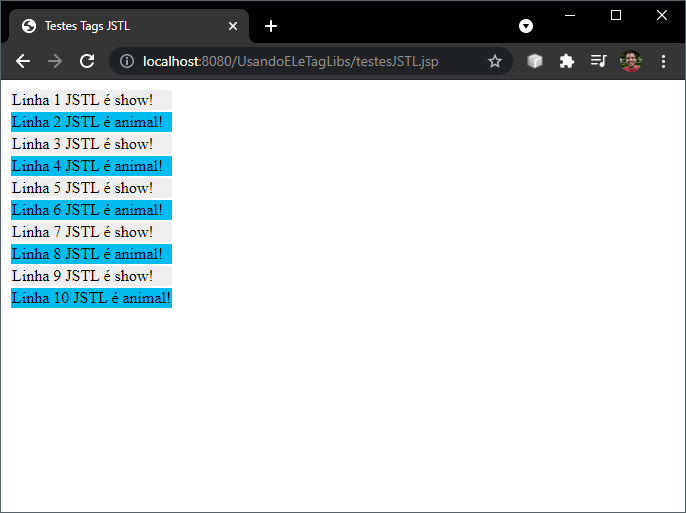
\includegraphics[scale=0.7]{imagens/cap03VisualizacaoTestesJSTL}
    \\\textbf{Fonte:} Elaborada pelo autor
    \label{fig:cap03VisualizacaoTestesJSTL}
\end{figure}
\FloatBarrier

Vamos analisar o código da Listagem~\thechapter.\ref{listagem:projetos/capitulo03/UsandoELeTagLibs/web/testesJSTL.jsp}. Talvez você tenha se assustado, mas não se preocupe, estou aqui para te explicar. Vamos começar pela primeira linha. Nessa linha, como em todos os JSPs que criamos até agora, usamos a diretiva \texttt{page}. As diretivas nos JSPs são delimitadas por \texttt{<\%@} e \texttt{\%>} e são usadas para realizar algumas configurações no Servlet que será gerado a partir do JSPs. A diretiva \texttt{page}, no nosso caso, é usada para configurar o \texttt{response} do Servlet, informando que ele vai conter um documento do tipo ``text/html'' (atributo \texttt{contentType}) e que o encoding utilizado (como os caracteres são codificados) é o UTF-8 (atributo \texttt{pageEncoding}). Veja que isso é análogo ao que estamos fazendo manualmente na primeira linha do método \texttt{processRequest} dos nossos Servlets.

Na linha 2 utilizamos a diretiva \texttt{taglib}. Essa diretiva vai permitir que nós digamos qual TagLib queremos utilizar. O atributo \texttt{uri} é usado para informarmos qual biblioteca de \textit{tags} queremos utilizar. No nosso caso, queremos utilizar as funcionalidades principais da JSTL, que são chamadas de ``core''. A \textit{Uniform Resource Identifier} (URI) para definir isso é a \texttt{http://java.sun.com/jsp/jstl/core}. O outro atributo, \texttt{prefix} (prefixo), nos permite definir um prefixo para usar as \textit{tags}. O prefixo padrão para a parte ``core'' da JSTL é ``c'', mas podemos usar o prefixo que quisermos. Para manter o padrão, iremos usar o ``c'' mesmo. Assim, quando qualquer desenvolvedor Web que conheça a JSTL bater o olho no código e ver alguma \textit{tag} que inicie com ``\texttt{c:}'' vai saber que a \textit{tag} que está sendo utilizada faz parte do core da JSTL.

Entre as linhas 12 e 20 definimos duas classes CSS. Sendo que uma usaremos para colorir o fundo das linhas pares de uma tabela, enquanto a outra será usada para colorir o fundo das linhas ímpares. A propriedade usada em ambas as classes é a \texttt{background} (fundo), sendo que em cada uma usamos uma cor diferente usando a notação \textit{Red Green Blue} (RGB) em hexadecimal. Nas linhas 25 e 40 delimitamos uma tabela.

\begin{saibaMais}
    Nunca ouviu falar de cores na notação em hexadecimal? De uma olhada nesses links: \url{http://dematte.at/colorPicker/}, \url{http://paletton.com/}, \url{https://pt.wikipedia.org/wiki/Tripleto_hexadecimal} e \url{http://en.wikipedia.org/wiki/Web_colors}
\end{saibaMais}

Na linha 26, usamos a \textit{tag} \texttt{c:forEach} (olhe o prefixo!), usada para iterar um determinado número de vezes ou sobre alguma lista de objetos. No nosso caso, queremos que o que está entre \texttt{<c:forEach>} e \texttt{</c:forEach>} seja executado dez vezes, pois definimos que a iteração deve iniciar em 1, usando o atributo \texttt{begin}, e ir até 10, usando o atributo \texttt{end}. Queremos também que o \textit{status} da iteração seja armazenado na variável ``i'', definida no atributo \texttt{varStatus}. Então temos um \texttt{for} que vai executar dez vezes. Durante estas dez iterações, vamos construir nossa tabela, inserindo linhas nela com apenas uma coluna, mas queremos que as linhas pares sejam coloridas usando a classe \texttt{linhaPar}, enquanto que as linhas ímpares sejam coloridas usando a classe \texttt{linhaImpar}. Sabemos que todo número par tem resto igual à zero numa divisão por dois, correto? Então precisamos saber em qual iteração estamos, calcular o resto e verificar se é zero. Se for, cria uma linha da tabela usando a classe \texttt{linhaPar}, caso contrário, usa \texttt{linhaImpar}.

Para criar séries de testes lógicos como numa estrutura \texttt{if/else if/else}, nós usamos a \textit{tag} \texttt{<c:choose>} (\textit{to choose} = escolher) e dentro dela colocamos as condições que queremos testar usando a \textit{tag} \texttt{<c:when>} que é equivalente aos \texttt{if’s} e \texttt{else if’s} e, por fim, se necessário, usamos a \textit{tag} \texttt{<c:otherwise>} que é equivalente ao \texttt{else}. Vamos analisar o código então: entre as linhas 27 e 38 nós definimos nossa estrutura condicional usando a \textit{tag} \texttt{<c:choose>}. Dentro dela, definimos na linha 28 uma \textit{tag} \texttt{<c:when>}, que testa (atributo \texttt{test}) se a divisão da propriedade \texttt{count} da variável \texttt{i} por dois é igual a zero (par). Note o uso da EL e que podemos executar operações aritméticas dentro dela! Se o resultado for \texttt{true}, o número é par e o conteúdo deste \texttt{<c:when>} é gerado, ou seja, uma linha da tabela usando a classe \texttt{linhaPar}. Caso contrário, como não temos mais nenhum \texttt{<c:when>}, é gerado o código dentro do \texttt{<c:otherwise>}, que por sua vez também gera uma linha da tabela, só que usando a classe \texttt{linhaImpar}. Fique à vontade para mudar o conteúdo gerado dentro de cada linha, bem como as classes.

Viu como não é tão complicado? Na verdade é bem simples e fácil de usar, mas precisamos praticar para ficarmos craques. Depois dessa introdução à EL e a JSTL, nós já estamos quase prontos para começarmos o nosso primeiro projeto Web de verdade, mas ainda temos que formalizar algumas coisas que serão vistas no próximo Capítulo. Novamente, não se esqueça de praticar o que fizemos até agora.  


\section{Resumo}

Neste Capítulo nós aprendemos a criar um formulário que teve seus dados tratados por um Servlet, que por sua vez redirecionou o fluxo da aplicação para outra página JSP, utilizada para mostrar os dados informados no formulário. Com isso, tivemos uma noção do que é a EL e como ela funciona. Depois aprendemos um pouco sobre as \textit{tags} padrão da especificação dos JSPs e, por fim, aprendemos utilizar a JSTL em nosso projeto, além de fazermos alguns testes. No próximo Capítulo vamos dar uma paradinha com os JSPs e Servlets para podermos aprender como estruturar um projeto Web que trabalha com banco de dados. Tenho certeza que você vai gostar bastante.


\section{Exercícios}

\begin{exercicioSemArquivo}{}{}{}
    Explique, com suas palavras, qual a importância da EL.
\end{exercicioSemArquivo}

\begin{exercicioSemArquivo}{}{}{}
    Justifique porque é melhor usar a JSTL ou qualquer outra TagLib ao invés de usar código Java diretamente nas JSPs.
\end{exercicioSemArquivo}

\section{Projetos}

\begin{projetoSemArquivo}{}{}{}
    Modifique o Projeto 1.1 do Capítulo 2 para executar da mesma forma que o projeto criado neste Capítulo, ou seja, o formulário deve submeter os dados para um Servlet, que por sua vez deve criar e enviar um objeto através do \texttt{request} para um JSP, que deve exibir ao usuário usando EL.
\end{projetoSemArquivo}

\begin{projetoSemArquivo}{}{}{}
    Modifique o Projeto 1.2 do Capítulo 2 para executar da mesma forma que o projeto criado neste Capítulo, ou seja, o formulário deve submeter os dados para um Servlet, que por sua vez deve criar e enviar um objeto através do \texttt{request} para um JSP, que deve exibir ao usuário usando EL.
\end{projetoSemArquivo}

\begin{projetoSemArquivo}{}{}{}
    Você já sabe que uma JSP na verdade é um Servlet não é mesmo? Será então que podemos definir na \texttt{action} de um formulário o endereço de um arquivo JSP ao invés de um Servlet? Crie um novo projeto Java Web, chamado ``JSPTrataFormulario'', onde você deve ter um formulário no \texttt{index.html} que contenha dois campos: nome e idade. A action deste formulário deve apontar para um arquivo JSP chamado ``exibeDadosForm.jsp'' (sem as aspas). Nesse arquivo, você deve mostrar os dados recebidos do formulário do \texttt{index.html} usando EL. Dica: para acessar os parâmetros do \texttt{request} usando EL, usa-se \texttt{\${param.nomeDoParametro}}. Por exemplo, o parâmetro idade é acessado usando \texttt{\${param.idade}}.
\end{projetoSemArquivo}

\begin{projetoSemArquivo}{}{}{}
    Crie um novo projeto Java Web, com o nome de ``TabelaArbitraria'', onde no \texttt{index.html} você deve ter um formulário que pede ao usuário que seja digita a quantidade de linhas e de colunas que ele deseja que uma tabela seja gerada. Aponte a \texttt{action} deste formulário para outro arquivo JSP, chamado ``montadorTabela.jsp'', que obtém os dados enviados pelo formulário do \texttt{index.html} usando EL e usa dois \texttt{<c:forEach>} aninhados para construir a tabela de dimensões arbitrárias. Monte a tabela somente se o tamanho de linhas e de colunas for maior que zero. Se não for, exiba uma mensagem ao usuário. Dica: para testar se duas condições são verdadeiras, ou seja, se \texttt{param.colunas > 0} e \texttt{param.linhas > 0}, use o operador \texttt{and} (e) da EL, enquanto o operador ``maior que'' é o \texttt{gt} (\textit{greater than}). Ou seja, \texttt{test="\${(param.linhas gt 0) and (param.colunas gt 0)}"}.
\end{projetoSemArquivo}
\chapter{Padrões de Projeto: \textit{Factory}, DAO e MVC}\label{cap:padroesDeProjeto}
\epigraph{``\textit{É longo o caminho que vai do projeto à coisa}''.}{Molière}

\lettrine[lines=4, lhang=0.1, lraise=0, loversize=0.2, findent=0.1em]{\textcolor{corTema}{N}}{ESTE} Capítulo teremos como objetivo entender e aplicar os Padrões de Projeto \textit{Factory}, DAO e MVC. Além disso iremos aprender a integrar o acesso à banco de dados em uma aplicação Java.


\section{Introdução}

A partir de agora iremos dar um passo importantíssimo em nossos estudos sobre desenvolvimento de software, pois iremos aprender a lidar com um banco de dados em um sistema de testes que iremos construir. Isso nos dará o embasamento necessário para que no Capítulo~\ref{cap:primeiroProjeto} nós consigamos fazer essa mesma integração em aplicações Web. Além de aprendermos a conectar nossa aplicação com uma base de dados, iremos aprender também alguns padrões de projeto que nos ajudarão a organizar nossa aplicação de forma a melhorar sua manutenção. 

Antes de começarmos a discussão e a implementação desses padrões, nós precisamos preparar nosso ambiente de desenvolvimento. O NetBeans já temos instalado. O Sistema Gerenciador de Banco de Dados (SGBD) que iremos utilizar, o MariaDB\footnote{Provavelmente você deve ter instalado na sua máquina o MariaDB que é distribuído junto ao XAMPP}/MySQL, você provavelmente já deve ter instalado também. Com isso pronto, precisamos instalar uma ferramenta para nos ajudar a criar nossa base de dados. Iremos utilizar o MySQL Workbench, uma ferramenta gratuita para gerenciamento do MariaDB/MySQL. 


\section{Preparando o Ambiente}\label{sec:preparandoAmbiente}

Para começar, vamos fazer o download da ferramenta. Acesse o endereço \url{https://dev.mysql.com/downloads/workbench/}, escolha Microsoft Windows como plataforma, que provavelmente é o sistema operacional que você está utilizando e clique no botão ``\textit{Download}''. Fazendo isso, você será direcionado para uma página onde é requisitado um nome de usuário e senha. Se você não quiser se cadastrar (não precisa), clique no link embaixo do formulário de \textit{login} onde está escrito ``\textit{No thanks, just start my download}''. O download do instalador será iniciado.

Baixou? Legal! Execute o instalador. Na época da elaboração desse livro, a última versão disponível era a \texttt{8.0.25}. Basta seguir os passos, fazendo a instalação completa. Ao terminar, deixe marcada a opção \destaque{\textit{Launch MySQL Workbench now}} e clique em \destaque{\textit{Finish}}. Aguarde o MySQL Workbench abrir. A interface principal da versão 8.0.25 do Workbench pode ser vista na Figura~\ref{fig:cap04MySQLWorkbench}.

\FloatBarrier
\begin{figure}[!htbp]
    \centering
    \caption{Interface principal do MySQL Workbench}
    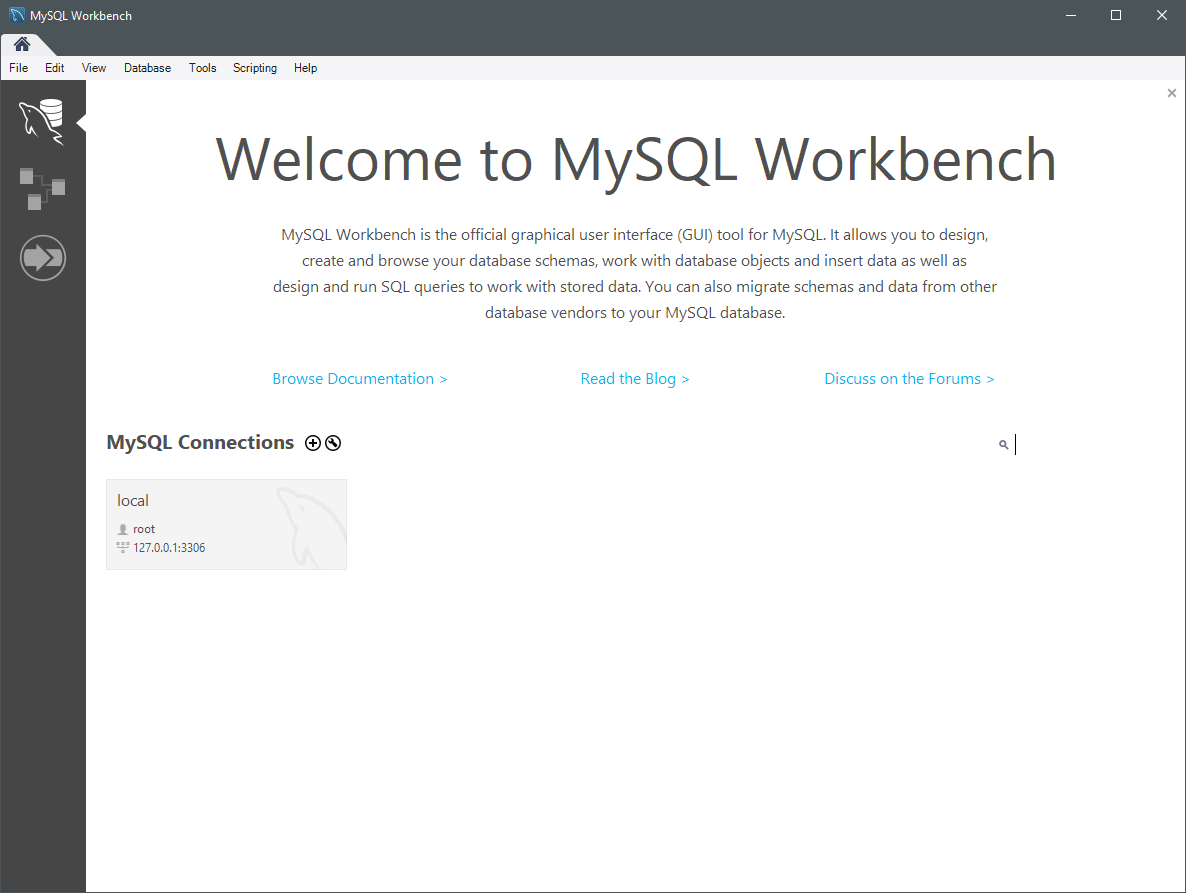
\includegraphics[scale=0.45]{imagens/cap04MySQLWorkbench}
    \\\textbf{Fonte:} Elaborada pelo autor
    \label{fig:cap04MySQLWorkbench}
\end{figure}
\FloatBarrier

Verifique se existe alguma instância configurada abaixo de \destaque{\textit{MySQL Connections}}, se não houver, clique em \destaque{\texttt{+}}. Um assistente aparecerá. Em \destaque{\textit{Connection Name:}} dê um nome para a conexão, pode ser qual você desejar. No meu caso, é ``localhost''. \destaque{\textit{Connection Method:}} deve ficar com a opção ``Standard (TCP/IP)'' selecionada. \destaque{\textit{Hostname:}} deve estar preenchido com o IP \texttt{127.0.0.1} que é o endereço de \textit{loopback}. Como o servidor está instalado na máquina que você está trabalhando, deixe como está. Em \destaque{\textit{Username:}} mantenha ``root'' e não será necessário configurar uma senha. Em \destaque{\textit{Port:}}, mantenha \texttt{3306}, que é a porta padrão que o MariaDB/MySQL ouve. Deixe \destaque{\textit{Default Schema:}} vazio. Note que estou assumindo que você está usando o MariaDB distribuído no XAMPP e que não realizou nenhuma mudança na instalação e no usuário administrador. Caso tenha realizado alguma alteração, você precisará replicá-las na configuração do MySQL Workbench. Clique no botão \destaque{\textit{Test Connection}}. A ferramenta vai avisar que há uma incompatibilidade de protocolos, pois ela está tentando conectar numa instância do MySQL, mas estamos rodando o MariaDB. Esse aviso pode ser ignorado, clicando em \destaque{\textit{Continue Anyway}}. Se tudo estiver correto, a conexão será bem sucedida, sendo avisada através de um diálogo com a mensagem ``\textit{Successfully made the MySQL connection}''. Lembre-se que o MariaDB/MySQL deve estar em execução! Por fim, clique no botão \destaque{\textit{OK}}, o diálogo será fechado e a conexão aparecerá.

Clique duas vezes na conexão criada. Novamente, será mostrado um aviso, dizendo sobre a incompatibilidade de protocolos. \textcolor{red}{\textbf{\underline{Não marque a opção} ``\textit{Don't show this message again}''}} e clique em \destaque{\textit{Continue Anyway}}. Pronto? Muito bem! Sempre que abrirmos o Workbench, essas configurações já estarão feitas, não se preocupe. Agora nós vamos criar uma base de dados para trabalharmos nos exemplos deste Capítulo.

Na interface que se abriu, do lado esquerdo, em \destaque{\textit{Navigator}} há duas abas que ficam abaixo. Uma é chamada \destaque{\textit{Administration}}, que é a que está selecionada por padrão, e outra chamada \destaque{\textit{Schemas}}. Clique em \destaque{\textit{Schemas}}. No aba de esquemas, na parte em branco, clique com o botão direito e escolha \destaque{\textit{Create Schema}}. Preencha o campo \destaque{\textit{Name:}} com ``\texttt{testes\_padroes}'' (sem as aspas) e deixe o campo \destaque{\textit{Charset/Collation:}} como ``Default Charset'' e ``Default Collation''. Clique em \destaque{\textit{Apply}}. Um diálogo será aberto para mostrar o código SQL que será executado. Clique em \destaque{\textit{Apply}} e se der tudo certo, clique em \destaque{\textit{Finish}}. A aba de criação de esquemas continuará aberta, podendo ser fechada. Ao terminar esse processo, o novo esquema (vamos chamar os esquemas de base de dados a partir de agora) será criado e estará listado na lista \destaque{\textit{SCHEMAS}}. Vamos configurar a base de dados que acabamos de criar como padrão, ou seja, as instruções SQL que realizarmos serão aplicados nessa base. Para isso, clique com o botão direito em \texttt{testes\_padroes} e escolha a opção \destaque{\textit{Set as Default Schema}}. Veja a Figura~\ref{fig:cap04SelecionandoEsquema}. Após fazer isso, o nome da base de dados ficará em negrito.

\FloatBarrier
\begin{figure}[!htbp]
    \centering
    \caption{Selecionando a base de dados \texttt{testes\_padroes}}
    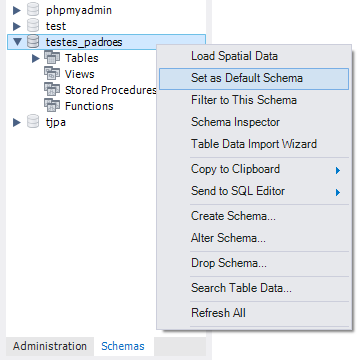
\includegraphics[scale=0.8]{imagens/cap04SelecionandoEsquema}
    \\\textbf{Fonte:} Elaborada pelo autor
    \label{fig:cap04SelecionandoEsquema}
\end{figure}
\FloatBarrier

Com a base \texttt{testes\_padroes} configurada como padrão, expanda-a e em \destaque{\textit{Tables}} clique com o botão direito e escolha \destaque{\textit{Create Table...}}. Vamos criar agora uma tabela que vai armazenar os dados de teste que iremos mexer durante este Capítulo. Preencha \destaque{\textit{Table Name:}} com ``pais'' (sem as aspas). \textit{Pais} é país, mas vamos omitir o acento tudo bem? Deixe os valores padrão nos campos \destaque{\textit{Charset/Collation:}}, \destaque{\textit{Engine:}} e \destaque{\textit{Comments:}}. Logo abaixo, clique duas vezes na primeira linha da coluna \destaque{\textit{Column Name}}. A ferramenta vai preencher o nome da primeira coluna automaticamente com o valor ``idpais''. Edite esse nome e deixe apenas ``id''. O tipo (Datatype) deve ficar como INT (inteiro) e as colunas \texttt{PK} (\textit{primary key}/chave primária), \texttt{NN} (\textit{not null}/não nulo) e \texttt{AI} (auto-increment/auto-incremento) devem ficar marcadas. Essa coluna da tabela será nossa chave primária. Agora vamos às outras colunas. Nossos países terão um nome e uma sigla. Então precisamos criar mais duas colunas, uma com nome de ``nome'' e a outra com nome de ``sigla''. A coluna ``nome'' terá o tipo \inlineSQLCode{VARCHAR(100)}, ou seja, um \inlineSQLCode{VARCHAR} de 100 posições e a coluna ``sigla'' terá o tipo \inlineSQLCode{VARCHAR(2}). Marque essas duas colunas como \texttt{NN}, ou seja, elas terão dados obrigatoriamente quando um país for ser inserido na tabela. Veja como ficou na Figura~\ref{fig:cap04CriandoTabelaPais}.

\FloatBarrier
\begin{figure}[!htbp]
    \centering
    \caption{Criando a tabela ``pais''}
    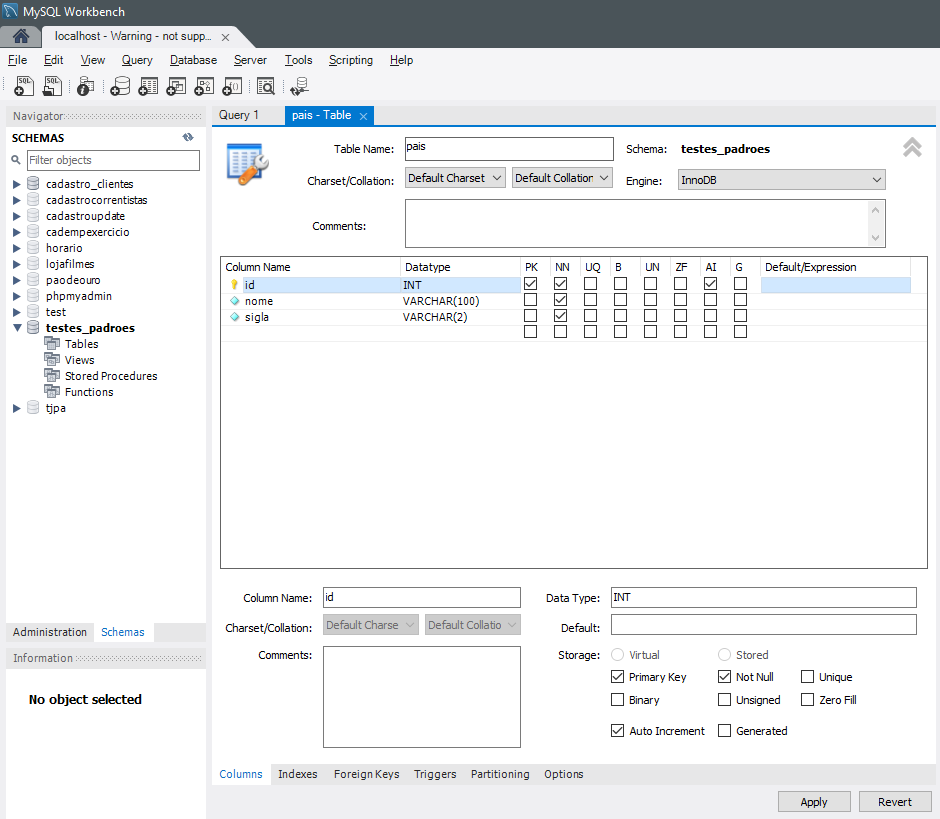
\includegraphics[scale=0.6]{imagens/cap04CriandoTabelaPais}
    \\\textbf{Fonte:} Elaborada pelo autor
    \label{fig:cap04CriandoTabelaPais}
\end{figure}
\FloatBarrier

Feito isso, clique em \destaque{\textit{Apply}}. Um diálogo será aberto para exibir o código SQL que será executado (Listagem~\thechapter.\ref{listagem:projetos/capitulo04/pais.sql}). Clique em \destaque{\textit{Apply}} e depois em \destaque{\textit{Finish}}. Pronto, criamos a nossa tabela para armazenar dados dos países, ela poderá ser vista do lado esquerdo, na aba \destaque{\textit{Schemas}}, dentro da base \texttt{testes\_padroes}. Deixe o Workbench aberto e abra o NetBeans. 

\sqlCode{Instrução \texttt{CREATE TABLE} para a tabela ``pais''}{projetos/capitulo04/pais.sql}

\section{Padrão de Projeto Factory}

Primeiramente, vamos criar um novo projeto no NetBeans, só que agora ele não será um projeto Web, pois o que vamos fazer não precisa ser em um projeto desse tipo. Siga os passos que você está acostumado a fazer ao criar um projeto Java Web, só que desta vez escolha \destaque{\textit{Java with Ant}} na categoria e \destaque{\textit{Java Application}} nos tipos de projeto. Dê o nome de ``PadroesEmPratica'' para o projeto. Não se esqueça de marcar a opção \destaque{\textit{Use Dedicated Folder for Storing Libraries}}.

Como iremos conectar no banco de dados MariaDB, precisamos adicionar no nosso projeto a biblioteca que implementa esse conector. Infelizmente o NetBeans não vem com essa biblioteca pronta para ser usada, então teremos que baixá-la e inseri-la no projeto. Para isso, primeiro baixe o arquivo \texttt{.jar} da bibliteca no endereço \url{NOME}. Com o arquivo baixado, clique com o botão direito no nó \destaque{\textit{Libraries}} e escolha a opção \destaque{\textit{Add Library...}}. No diálogo que foi aberto, clique em \destaque{\textit{Create...}}. No diálogo que vai se abrir, preencha \destaque{\textit{Library Name:}} com ``MariaDB-ConnectorJ-2.7.3'' (ou o nome que você quiser) e em \destaque{\textit{Library Type}} deixe ``Class Libraries'' e clique em \destaque{\textit{OK}}. Mais um diálogo será aberto. Clique no botão \destaque{\textit{Add JAR/Folder...}} e procure pelo arquivo \texttt{.jar} da biblioteca que acabou de baixar. Selecione-se o clique em \destaque{\textit{Add JAR/Folder}}. Ao clicar nesse botão, um alerta perguntará se você que criar um diretório na pasta de bibliotecas do projeto, clique em \destaque{\textit{Yes}}. Agora clique no botão \destaque{\textit{OK}} do diálogo \destaque{\textit{Customize Library}} e, agora que a biblioteca foi criada, selecione-a no diálogo \destaque{\textit{Add Library}} e clique no botão \destaque{\textit{Add Library}}. Perceba que ao fazer isso, um aparecerá um novo nó dentro da pasta \destaque{\textit{Libraries}} do projeto com o nome da bibliteca que foi criada e adicionada.

A partir de agora, podemos conectar ao banco de dados a partir do nosso código. Como você deve saber, para que possamos usar um banco de dados em Java, nós usamos uma especificação chamada \textit{Java Database Connectivity} (JDBC). Essa especificação deve ser implementada pelos fabricantes dos SGBDs, permitindo assim que os programas feitos em Java possam se comunicar com estes SGBDs. Normalmente, esses pacotes que implementam o JDBC são chamados de ``Drivers JDBC'' e são obtidos nos sites dos fabricantes dos SGBDs.

A questão agora é: ``Como conectar no banco de dados?''. Para que possamos conectar no MariaDB, existem uma série de ``comandos'' que precisamos fazer cada vez que queremos estabelecer uma conexão. Você, como desenvolvedor, sabe que uma boa prática de programação é encapsular trechos de código que fazem uma determinada tarefa em funções e que as funções em Java são chamadas de métodos.

Legal, mas e o que o tal do ``padrão de projeto'' tem haver com isso? Ou melhor, o que é um padrão de projeto? O termo padrão de projeto (\textit{design pattern} em inglês) foi criado por Christopher Alexander \cite{Alexander1977} na década de 1970 para designar soluções de sucesso para problemas recorrentes na área da arquitetura. Alexander definiu nessa época uma série de padrões que apresentavam soluções padrão para problemas que aconteciam de forma corriqueira, sendo que uma série de padrões correlatos foram o que podemos chamar de linguagem de padrões. A partir do termo cunhado por Alexander, alguns programadores começaram a criar padrões de projeto para a computação, iniciando esse trabalho do domínio da programação orientada a objetos.

O livro ``Padrões de Projeto: Soluções Reutilizáveis de Software Orientado a Objetos'' \cite{Gamma2000} é a referência básica para os padrões de projeto criados para resolver problemas relacionados ao desenvolvimento orientado a objetos. A partir de agora, quando você ler ``padrão de projeto'', entenda que estarei falando de padrões relacionados ao desenvolvimento de software orientado a objetos, tudo bem? Sendo assim, o primeiro padrão que iremos aprender se chama \textit{Factory} (fábrica). 

Vamos entender o contexto do padrão. Imagine que no seu programa você precisa criar e utilizar um determinado tipo de objeto muitas e muitas vezes e que este objeto precisa ser inicializado com uma série de valores, sendo que esses valores normalmente são sempre os mesmos. Assim, cada vez que você instância esse objeto, você precisa executar uma determinada quantidade de código. Como resolver isso? Criar um método que faça essa tarefa é uma boa solução não é mesmo? Mas em qual classe eu vou escrever esse método? No padrão \textit{Factory}, nós criamos classes especializadas que serão fábricas de objetos e que terão um método que executará a tarefa da fábrica, ou seja, criar um determinado tipo de objeto.

No nosso projeto, um tipo de objeto que usaremos muito, é um objeto que representa a conexão entre nosso programa escrito em Java e o SGBD. Sendo assim, nós precisamos de uma fábrica de conexões! Vamos implementar a fábrica? No projeto que você criou agora a pouco, o NetBeans gerou por padrão um pacote chamado ``padroesempratica'' dentro da pasta \destaque{\textit{Source Packages}}. Crie dentro deste pacote outro com o nome de ``jdbc'' (sem as aspas) e dentro do pacote ``padroesempratica.jdbc'', crie uma classe Java com o nome de ``ConnectionFactory'' (sem as aspas). Essa classe conterá o método que vai fabricar a conexão. Veja o código dela na ListagemListagem~\thechapter.\ref{listagem:projetos/capitulo04/PadroesEmPratica/src/padroesempratica/jdbc/ConnectionFactory.java}.

\javaCode{Uma fábrica de conexões (\texttt{padroesempratica/jdbc/ ConnectionFacotory.java})}{projetos/capitulo04/PadroesEmPratica/src/padroesempratica/jdbc/ConnectionFactory.java}

Copiou o código? Ótimo! Esta classe tem um método estático chamado \texttt{getConnection()} que vai fabricar a conexão para nós e que caso ocorra algum problema, vai lançar uma exceção do tipo SQLException. Toda vez que chamarmos esse método, ele vai retornar uma nova conexão para nós e o Driver JDBC apropriado será carregado automaticamente pelo \texttt{DriverManager}. 

Agora precisamos testar esse método para ver se não está havendo nenhum erro. Clique novamente com o botão direito no pacote ``padroesempratica'' e crie um novo pacote chamado ``testes''. Dentro do pacote ``padroesempratica.testes'', crie uma classe chamada ``TesteConnectionFactory''. Como você deve saber, para que uma classe em Java possa ser executada, nós precisamos implementar o método \inlineJavaCode{main(...)} com uma determinada assinatura. O que vamos fazer no método \inlineJavaCode{main(...)} da classe ``TesteConnectionFactory'' é tentar criar uma conexão e ver se nenhum erro é retornado. Na Listagem~\thechapter.\ref{listagem:projetos/capitulo04/PadroesEmPratica/src/padroesempratica/testes/TesteConnectionFactory.java} você pode ver o código desta classe.

\javaCode{Classe para teste de conexão (\texttt{padroesempratica/testes/ TesteConnectionFactory.java})}{projetos/capitulo04/PadroesEmPratica/src/padroesempratica/testes/TesteConnectionFactory.java}

Copie o código para a classe e salve o arquivo. Para executarmos apenas uma classe que tem o método \inlineJavaCode{main(...)}, basta clicar com o botão direito no editor e escolhe a opção \destaque{\textit{Run File}}, ou então, com o arquivo aberto no editor, usar o atalho \texttt{<Shift+F6>}. Fazendo isso, a classe vai ser compilada e executada pelo NetBeans. Se tudo estiver correto, você verá na saída a mensagem ``Conexão criada com sucesso!''. Deu erro? Verifique se o código da classe \texttt{ConnectionFactory} está correto e se a senha do usuário \texttt{root}, definida dentro do método \inlineJavaCode{getConnection()} está correta. No nosso caso, ela é vazia. Agora que está tudo certo, vamos simular um erro. Entre na classe \texttt{ConnectionFactory} e coloque uma senha inválida (terceiro parâmetro do método \inlineJavaCode{getConnection(...)} de \texttt{DriverManagaer}) para o usuário \texttt{root}, por exemplo, ``123''. Volte na classe de testes e execute-a novamente (\texttt{<Shift+F6>}). Gerou um erro não foi? A mensagem ``Erro ao tentar criar a conexão!'' deve ter sido exibida, seguida de várias linhas que explicam o erro ocorrido. A primeira linha dos erros diz que o acesso foi negado para o usuário ``root@localhost'' não foi? Por que aconteceu isso? Porque a senha está errada! Volte na fábrica de conexões e coloque a senha correta (vazia). Teste novamente. Agora deve estar tudo certo.

Legal, temos uma fábrica de conexões, mas do que adianta uma fábrica de alguma coisa se a gente não usar o que é fabricado? Vamos para o próximo padrão, onde iremos organizar uma camada de persistência para nossa aplicação e usaremos a fábrica de conexões para viabilizar a comunicação entre nossa aplicação e o SGBD.


\section{Padrão de Projeto \textit{Data Access Object} (DAO)}

Quando temos o nosso primeiro contato com JDBC, normalmente nos é ensinado a colocar todo o código SQL que vai executar uma determinada operação em um método que trata o ``clique'' de um botão. Sendo assim, imagine uma interface gráfica de uma aplicação \textit{desktop} (em Swing) onde poderíamos criar, alterar e/ou excluir países. Quando implementamos o botão responsável por criar um novo país, somos ensinados a inserir todo o código SQL para fazer isso, sendo que esse código é implementado usando uma instrução \inlineSQLCode{INSERT}. O mesmo aconteceria para os botões alterar e excluir. Será que essa é a melhor solução? Será que a classe que implementa nossa interface gráfica tem que ter essa responsabilidade, ou seja, lidar com SQL? E se por algum motivo nós quiséssemos usar o código para criar um novo país em alguma outra janela? Teríamos que copiar o código de inserção novamente? Tenho certeza que para essa última pergunta você já deve ter respondido mentalmente que ``NÃO!'', pois podemos criar métodos que executariam essa operação, mas então te pergunto: Como fazer isso?

Para resolver esse problema, existe um padrão de projeto onde a ideia é isolar todo acesso ao banco de dados em classes que seriam responsáveis em fazer a comunicação entre a aplicação Java, ou qualquer aplicação escrita usando uma linguagem orientada a objetos, e o banco de dados. Esse padrão se chama \textit{Data Access Object} (DAO), sendo este um dos mais famosos. Vamos aprender como implementá-lo?

Um objeto do tipo DAO deve ter a capacidade de executar as operações básicas sobre uma determinada tabela de um banco de dados. Essas operações são comumente chamadas de ``CRUD'' que vem de ``\textit{Create, Read, Update e Delete}'' (Criar, Ler, Atualizar e Excluir). Praticamente cada tabela do nosso banco de dados terá no lado da aplicação uma classe implementada que representará um registro da tabela (tabela ``pais'', classe Pais) por meio de um objeto do tipo em questão, além de ter uma classe DAO que vai manipular esses objetos. Como precisamos definir essas quatro operações básicas que cada DAO vai conter, vamos criar uma classe abstrata que servirá de modelo.

No pacote ``padroesempratica'', crie um novo pacote chamado ``dao''. Dentro do pacote ``padroesempratica.dao'', crie uma classe chamada ``DAO'' e copie o código apresentado na Listagem~\thechapter.\ref{listagem:projetos/capitulo04/PadroesEmPratica/src/padroesempratica/dao/DAO.java}.

\javaCode{Implementação da classe abstrata DAO (\texttt{padroesempratica/dao/DAO.java})}{projetos/capitulo04/PadroesEmPratica/src/padroesempratica/dao/DAO.java}

Copiou o código? Ótimo! Vamos entendê-lo. Na linha 13 definimos uma classe abstrata\footnote{Classes abstratas não podem ser instanciadas, são usadas como modelos.} chamada DAO que diz que toda classe que for implementá-la deve fornecer um tipo genérico chamado de \texttt{Tipo}. As construções entre \inlineJavaCode{<} e \inlineJavaCode{>} são chamadas de ``Tipos Genéricos'' em Java. Note que o tipo \texttt{Tipo} é usado em todo o corpo da classe. Está confuso? Acalme-se, logo você vai entender.

Na linha 16 é declarada uma variável de instância que referenciará uma conexão, que sempre será obtida usando o método \inlineJavaCode{getConnection()} definido na linha 39. Observe que poderíamos ter declarado essa conexão como \inlineJavaCode{protected}, mas vamos deixá-la como \inlineJavaCode{private} e usar o método \inlineJavaCode{getConnection()} para obtê-la. Na linha 49 é definido o método para fechar a conexão, afinal, sempre depois de usarmos uma conexão, precisamos fechá-la.

Veja que no construtor da classe a conexão é obtida usando a fábrica que criamos na Seção anterior! Esse construtor será executado quando instanciarmos os objetos das classes que estenderem esse DAO, então, quando criarmos nossos objetos DAO, uma conexão com o banco de dados será estabelecida.

A partir da linha 62 são definidos todos os métodos CRUD deste DAO genérico. Note que temos dois métodos que correspondem à parte ``R'' do CRUD, onde um obtém todas as entidades cadastradas e outro obtém apenas uma usando como base seu identificador.

Com o DAO genérico pronto, vamos implementar a classe que vai representar a tabela ``pais''. Crie um novo pacote chamado ``entidades'' dentro do pacote ``padroesempratica''. Dentro do pacote ``padroesempratica.entidades'', crie uma classe chamada ``Pais'' (sem as aspas). Os objetos dessa classe representarão registros da tabela ``pais'', sendo assim, precisamos que essa classe tenha os mesmos atributos da tabela correspondente. Lembre-se que na tabela ``pais'' nós definimos três colunas: id (\inlineSQLCode{INT}), nome (\inlineSQLCode{VARCHAR}) e sigla (\inlineSQLCode{VARCHAR}). Na nossa classe, iremos usar o tipo \inlineJavaCode{int} como tipo correspondente ao \inlineSQLCode{INT} da tabela. Para o tipo \inlineSQLCode{VARCHAR}, usaremos \inlineJavaCode{String}. Veja na Listagem~\thechapter.\ref{listagem:projetos/capitulo04/parciais/Pais.java} como deve ficar a implementação parcial da classe \texttt{Pais}.

\javaCode{Implementação parcial da classe Pais (\texttt{padroesempratica/entidades/Pais.java})}{projetos/capitulo04/parciais/Pais.java}

Tenho certeza que você se lembra da discussão sobre o padrão JavaBeans não é mesmo? Onde foi dito que devemos expor ao mundo ``fora da classe'' os atributos que nós queremos que possam ser configurados e obtidos por seus utilizadores? Da primeira vez que falamos sobre isso, nós implementamos manualmente cada método \texttt{set} e \texttt{get} correspondente a um campo privado não foi? Como essa tarefa é muito corriqueira, o NetBeans tem uma funcionalidade que faz isso automaticamente para nós. Com a classe implementada, como exibido na Listagem~\thechapter.\ref{listagem:projetos/capitulo04/parciais/Pais.java}, clique com o botão direito no editor e escolha \destaque{\textit{Insert Code...}}. Ao clicar nesta opção, uma pequena lista com o nome de \destaque{\textit{Generate}} será exibida no editor. Nessa lista, escolha a opção \destaque{\textit{Getter and Setter...}}. Adivinhe o que vamos fazer? Gerar os métodos \texttt{get} e \texttt{set} para cada campo da classe! Fazendo isso, um diálogo será exibido, mostrando todos os campos privados da classe. Marque cada um dos campos clicando na caixa de seleção correspondente, ou então, a classe inteira e clique no botão \destaque{\textit{Generate}}. Veja o que aconteceu! A IDE gerou o código dos \texttt{gets} e \texttt{sets} para nós! Segue na Listagem~\thechapter.\ref{listagem:projetos/capitulo04/PadroesEmPratica/src/padroesempratica/entidades/Pais.java} o código completo da classe Pais.

\javaCode{Implementação da classe Pais (\texttt{padroesempratica/ entidades/Pais.java})}{projetos/capitulo04/PadroesEmPratica/src/padroesempratica/entidades/Pais.java}

Muito legal não é mesmo? Agora que temos a classe que representa a estrutura da tabela ``pais'' da nossa base de dados, vamos implementar nosso primeiro DAO concreto, ou seja, uma classe que vai estender a classe abstrata DAO. Novamente, no pacote ``padroesempratica.dao'', crie uma classe chamada ``PaisDAO'' (sem as aspas). Essa classe irá lidar com os objetos do tipo \texttt{Pais}, fazendo a ponte entre nossos objetos e o banco de dados. Com a classe criada, copie o código apresentado na Listagem~\thechapter.\ref{listagem:projetos/capitulo04/parciais/PaisDAOP1.java}.

\javaCode{Implementação parcial da classe PaisDAO (\texttt{padroesempratica/dao/PaisDAO.java})}{projetos/capitulo04/parciais/PaisDAOP1.java}

Veja que nosso \texttt{PaisDAO} vai estender \texttt{DAO}, informando como tipo a classe \texttt{Pais} (\texttt{DAO<Pais>}). Ao copiar o código, você perceberá que o NetBeans vai reclamar, dizendo que tem um erro na classe. O nome da classe ficará destacado em vermelho. Passe o mouse por cima do nome e aguarde. Será exibida a causa do erro. No erro, é dito que a classe \texttt{PaisDAO} não implementa todos os métodos abstratos da classe \texttt{DAO} e isso é verdade, visto que como estamos estendendo a classe \texttt{DAO}, precisamos implementar todos os métodos abstratos que foram definidos nela e ainda não fizemos isso. Teríamos então que implementar manualmente todos os métodos marcados como abstratos na classe \texttt{DAO}. Ao invés de fazermos isso manualmente, o NetBeans pode nos ajudar novamente. Veja que na linha do erro, à esquerda, é mostrada uma pequena lâmpada com uma bolinha vermelha. Clique nela. Ao clicar, o NetBeans vai listar as alternativas que ele pode executar para resolver o erro. Veja a Figura~\ref{fig:cap04ImplementacaoAutomatica}.

\FloatBarrier
\begin{figure}[!htbp]
    \centering
    \caption{Implementando automaticamente os métodos abstratos de DAO}
    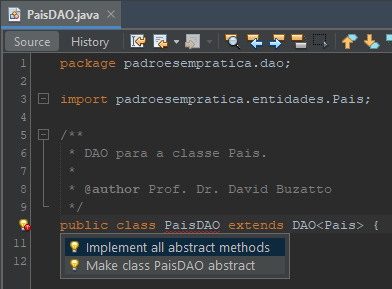
\includegraphics[scale=1]{imagens/cap04ImplementacaoAutomatica}
    \\\textbf{Fonte:} Elaborada pelo autor
    \label{fig:cap04ImplementacaoAutomatica}
\end{figure}
\FloatBarrier

Clique na opção \destaque{\textit{Implement all abstract methods}} e, novamente, como num passe de mágica, o NetBeans gera todo o esqueleto da classe para nós, criando uma implementação padrão para cada método abstrato da classe \texttt{DAO}. Mesmo ao fazer isso, o NetBeans continua reclamando que existe um erro. Nesse caso, é dito que é lançada uma exceção no construtor padrão\footnote{O construtor padrão é o construtor que não tem nenhum parâmetro.}. Você se lembra que lá no \texttt{DAO} genérico nós temos um construtor que cria a conexão e que ele lança uma \texttt{SQLException}? Pois bem, quando criamos um objeto de uma determinada classe, o construtor da superclasse da classe em questão a primeira coisa que será executada. Como estendemos \texttt{DAO} em \texttt{PaisDAO}, ao tentarmos instanciar um objeto do tipo \texttt{PaisDAO}, o construtor de \texttt{PaisDAO} será executado, além do construtor de \texttt{DAO}, que é sua superclasse. Como o construtor de \texttt{DAO} lança uma exceção caso ocorra algum problema, nós precisamos ou tratar ou dizer que o construtor de \texttt{PaisDAO} também lança esse tipo de exceção. Nós iremos usar a segunda abordagem. Para isso, basta implementar o construtor padrão de \texttt{PaisDAO} e dizer que ele lança esse tipo de exceção. Sendo assim, segue na Listagem~\thechapter.\ref{listagem:projetos/capitulo04/parciais/PaisDAOP2.java} a implementação que temos até agora da classe \texttt{PaisDAO}.

\javaCode{Implementação parcial da classe PaisDAO com o construtor padrão (\texttt{padroesempratica/dao/PaisDAO.java})}{projetos/capitulo04/parciais/PaisDAOP2.java}

Muito bom! Até agora preparamos toda o esqueleto do nosso \texttt{PaisDAO}, mas SQL que é bom, nada. Vamos agora implementar nosso primeiro método do CRUD, o ``salvar''. Antes de implementar o método ``salvar'', importe a classe \texttt{java.sql.PreparedStatement}. Na Listagem~\thechapter.\ref{listagem:projetos/capitulo04/parciais/PaisDAOSalvar.java} pode ser vista a implementação do método \texttt{salvar} da classe \texttt{PaisDAO}.

\javaCode{Implementação do método ``salvar'' da classe PaisDAO (\texttt{padroesempratica/dao/PaisDAO.java})}{projetos/capitulo04/parciais/PaisDAOSalvar.java}

Vamos analisar o código para ver o que está acontecendo. Na linha 20 está definida a assinatura do método. O método \texttt{salvar} recebe um parâmetro do tipo \texttt{Pais}, sendo que os dados do objeto passado nesse parâmetro serão persistidos no banco de dados. Nas linhas 22 e 23 é definida a instrução \inlineSQLCode{INSERT} do banco de dados. Como a coluna \texttt{id} da tabela \texttt{pais} foi definida como auto-incremento, nós não precisamos fornecê-la. Ao invés de definirmos manualmente os valores das colunas nome e sigla, perceba que utilizamos sinais de interrogação, indicando que no lugar de cada ponto de interrogação será trocado pelo valor correto. Na linha 25 é criado um \texttt{PreparedStatement} a partir da conexão do \texttt{DAO} usando o código SQL que foi definido nas linhas 22 e 23. Na linha 26, o primeiro parâmetro do código SQL (primeiro ponto de interrogação) é ``trocado'' pelo valor retornado pelo método \inlineJavaCode{getNome()} do objeto referenciado por \texttt{obj} que é do tipo \texttt{Pais}. A mesma coisa acontece na linha 27, onde o segundo parâmetro do código SQL (segundo ponto de interrogação) é ``trocado'' pelo valor retornado pelo método \inlineJavaCode{getSigla()}. Com o \texttt{PreparedStatement} configurado, na linha 29 mandamos que seja executado o \texttt{PreparedStatement}. Por fim, na linha 30, fechamos o \texttt{PreparedStatement}. Fácil não é?

Vamos testar? No pacote ``padroesempratica.testes'', crie uma classe chamada \texttt{TestePaisDAO} e copie o código da Listagem~\thechapter.\ref{listagem:projetos/capitulo04/PadroesEmPratica/src/padroesempratica/testes/TestePaisDAO.java}.

\javaCode{Código de teste para o PaisDAO (\texttt{padroesempratica/ testes/TestePaisDAO.java})}{projetos/capitulo04/PadroesEmPratica/src/padroesempratica/testes/TestePaisDAO.java}

Copiou o código? Execute a classe (botão direito no arquivo, \destaque{\textit{Run File}} ou \texttt{<Shift+F6>}). Se tudo estiver correto, a classe será compilada e executada e nenhum erro será emitido. Fazendo isso, um novo registro na tabela ``pais'' será inserido. Vamos confirmar isso? No MySQL Workbench deve haver um editor SQL já aberto. Se não houver, abra um clicando no ícone com uma folha com a sigla SQL e um sinal de \texttt{+}. Confirme também se a base de dados ``testes\_padroes'' está configurado como padrão ou está ativa. No editor, digite \inlineSQLCode{SELECT * FROM pais;} e clique no botão que tem um desenho de um raio na barra de ferramentas da aba do editor. O código SQL digitado será executado e o resultado será exibido logo abaixo. Veja a Figura~\ref{fig:cap04ExecucaoSelect}.

\FloatBarrier
\begin{figure}[!htbp]
    \centering
    \caption{Fazendo uma consulta do MySQL Workbench}
    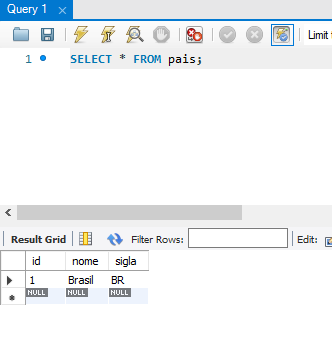
\includegraphics[scale=1]{imagens/cap04ExecucaoSelect}
    \\\textbf{Fonte:} Elaborada pelo autor
    \label{fig:cap04ExecucaoSelect}
\end{figure}
\FloatBarrier

Muito bem! Nosso método \texttt{salvar} de \texttt{PaisDAO} está funcionando corretamente. Vamos analisar o código da Listagem~\thechapter.\ref{listagem:projetos/capitulo04/PadroesEmPratica/src/padroesempratica/testes/TestePaisDAO.java}. Entre as linhas 16 e 18 instanciamos e configuramos um objeto do tipo \texttt{Pais}. O nome desse país é \texttt{Brasil} e a sigla é \texttt{BR}. Na linha 20, declaramos uma referência do tipo \texttt{PaisDAO} que foi inicializada com \inlineJavaCode{null}. Como todo o código dos métodos do \texttt{DAO} podem lançar uma exceção do tipo \texttt{SQLException}, temos que usar um bloco \inlineJavaCode{try}. Na linha 24 instanciamos o \texttt{PaisDAO} e na linha 25 passamos o objeto do tipo \texttt{Pais} que criamos para o método ``salvar'' do \texttt{DAO}, que por sua vez vai executar o código SQL que definimos. Caso ocorra algum problema durante a execução de uma dessas duas linhas, o \inlineJavaCode{catch} que ouve exceções do tipo \texttt{SQLException} captura o erro e manda mostrar esses problemas dando um \inlineJavaCode{printStackTrace()} no objeto que representa a exceção. Por fim, temos um bloco \inlineJavaCode{finally} que trata do fechamento da conexão. Sempre quando usarmos um \texttt{DAO}, precisamos fechar sua conexão quando terminarmos de usar. Na linha 31 verifica-se se o \texttt{dao} aponta para \inlineJavaCode{null}. Se não apontar, tenta fechar a conexão, que também pode lançar uma exceção do tipo \texttt{SQLException} e que é tratada dentro do bloco \inlineJavaCode{try} que está aninhado no \inlineJavaCode{finally}.

Agora que já criamos e testamos nosso primeiro método do \texttt{PaisDAO}, vamos implementar o restante dos métodos. Os métodos de pesquisa (``R'' do CRUD) serão um pouco diferente, sendo assim, eu os discutirei depois. Vamos lá, copie o restante do código para que seu \texttt{PaisDAO} fique igual ao da Listagem~\thechapter.\ref{listagem:projetos/capitulo04/PadroesEmPratica/src/padroesempratica/dao/PaisDAO.java}.

\javaCode{Implementação da classe PaisDAO (\texttt{padroesempratica/ dao/PaisDAO.java})}{projetos/capitulo04/PadroesEmPratica/src/padroesempratica/dao/PaisDAO.java}

Não se esqueça de importar as classes \texttt{java.sql.ResultSet}, \texttt{java.util.ArrayList} e \texttt{java.util.List}. Para finalizar essa seção, vamos discutir o código da Listagem~\thechapter.\ref{listagem:projetos/capitulo04/PadroesEmPratica/src/padroesempratica/dao/PaisDAO.java}. O método \inlineJavaCode{listarTodos()} retorna uma lista que pode conter apenar objetos do tipo \texttt{Pais}. Essa lista que será retornada é instanciada e inicializada na linha 72. Neste momento, temos a lista de objetos do tipo \texttt{Pais}, só que ela ainda está vazia. Na linha 75, cria-se o \texttt{PreparedStatement} com o SQL que foi definido na linha 73 e, na linha 75, executamos o \texttt{PreparedStatement} usando o método \inlineJavaCode{executeQuery()}, que retorna um objeto do tipo \texttt{ResultSet}. Os objetos do tipo \texttt{ResultSet} representam os resultados que são retornados em consultas SQL (instrução \inlineSQLCode{SELECT}). Na linha 78 usamos um \inlineJavaCode{while}, que é executado enquanto \inlineJavaCode{rs.next()} retornar \inlineJavaCode{true}. Na primeira vez que \inlineJavaCode{rs.next()} é invocado, o ponteiro de registros do \texttt{ResultSet} passa a apontar para o primeiro resultado obtido na consulta. Dentro do \inlineJavaCode{while}, entre as linhas 80 e 83, nós criamos um objeto do tipo \texttt{Pais} e configuramos seus dados a partir dos dados obtidos no \texttt{ResultSet}, usando o método apropriado para cada tipo de cada coluna. Na linha 85, o objeto \texttt{Pais} que acabou de ser criado e configurado é inserido na lista. O corpo do \inlineJavaCode{while} é repetido até que \inlineJavaCode{rs.next()} retorne \inlineJavaCode{false}, ou seja, quando todos os resultados da consulta foram obtidos. Nesse ponto, temos a lista de objetos completa. Nas linhas 89 e 90 são fechados o \texttt{ResultSet} e o \texttt{PreparedStatement}. Por fim, na linha 92, a lista com os objetos do tipo \texttt{Pais} é retornada.

Note que o método \inlineJavaCode{obterPorId( int id )} tem uma implementação muito parecida com o método \inlineJavaCode{listarTodos()}, só que no caso do \texttt{obterPorId}, apenas um objeto pode ser retornado, visto que cada registro da tabela \texttt{pais} tem um identificador específico. Caso o \texttt{id} passado como parâmetro não represente um registro da tabela \texttt{pais}, o método retorna \inlineJavaCode{null}.

Agora, como exercício, modifique a classe \texttt{TestePaisDAO} para testar todos os métodos que foram implementados. Verifique se todos estão corretos usando o MySQL Workbench para comparar os resultados obtidos. Tente entender a implementação de cada método do CRUD. Não fez o exercício? Então faça! Ele não é opcional.

Viu só que legal? Com tudo isso que fizemos, conseguimos isolar toda a camada de persistência da nossa aplicação. Para cada tabela nova que tivermos na base de dados, precisamos implementar a classe correspondente à tabela (que chamamos de entidade) e a classe DAO que vai manipular os objetos da classe criada e fazer o intercâmbio entre o mundo orientado a objetos com o mundo relacional. Essa comunicação entre objetos e o modelo relacional é chamada de Object-Relational Mapping (ORM). Existem alguns \textit{frameworks} que automatizam esse processo, gerando todo o código SQL automaticamente para nós. Infelizmente não teremos tempo para aprendê-los. Um desses \textit{frameworks} é o Hibernate.

\begin{saibaMais}
    Quer saber mais sobre ORM? Dê uma olhada nesses \textit{links}: \url{http://pt.wikipedia.org/wiki/Mapeamento_objeto-relacional}, \url{http://en.wikipedia.org/wiki/Object-relational_mapping}, \url{http://www.hibernate.org/}
\end{saibaMais}

Estamos quase acabando! Vamos para o último padrão de projeto.


\section{Padrão de Projeto \textit{Model-View-Controller} (MVC)}


O padrão MVC é um padrão muito utilizado no desenvolvimento de aplicações que utilizam linguagens orientadas a objetos. Este padrão ajuda os desenvolvedores a separar as regras de negócio da aplicação, ou seja, as regras de como os dados devem se armazenados, qual a ordem que devem ser gravados etc., da lógica de apresentação desses dados, ou seja, como eles serão exibidos aos usuários do sistema. Essa separação se dá utilizando três camadas: 

\begin{itemize}

    \item \textbf{\textit{Model} (Modelo):} A camada \textit{Model} é usada para organizar como os dados são armazenados e gerenciados dentro da aplicação. No exemplo que construímos durante este Capítulo, as classes \texttt{Pais} e \texttt{PaisDAO} fazem parte do modelo;
    
    \item \textbf{\textit{View} (Visualização):} Essa camada organiza os recursos utilizados para exibir ao usuário os dados que são gerenciados pela camada de modelo;
    
    \item \textbf{\textit{Controller} (Controle):} A camada \textit{Controller}, como o próprio nome já diz, é responsável por controlar o fluxo de execução da aplicação.
    
\end{itemize}

A partir dessas definições, nós podemos ver nitidamente, nos exemplos que estamos construindo desde o início da disciplina, qual recurso faz parte de cada camada. A entidade Pais faz parte do modelo. Uma JSP faz parte da visualização, pois é usada pelo usuário tanto para inserir dados no sistema quanto para visualizá-los. Os Servlets que construímos fazem parte do controle, pois são eles que recebem os dados, os utilizam usando a camada de modelo e decidem para onde o fluxo da aplicação deve ser direcionado, por exemplo, uma página JSP que vai exibir a saída gerada por eles.

Essa foi uma pequena introdução do MVC, pois durante Capítulo~\ref{cap:primeiroProjeto} nós iremos usá-lo extensivamente no projeto que iremos criar. Tenho certeza que você vai achar muito legal e útil! Como de costume, pratique o que você aprendeu durante este Capítulo com as atividades de aprendizagem.


\section{Resumo}

Neste Capítulo demos um passo muito importante na nossa vida como desenvolvedores. Nós aprendemos que existem os chamados ``padrões de projeto'' ou ``\textit{design patterns}'', que são padrões que guiam os desenvolvedores na solução de problemas recorrentes através do uso de soluções de sucesso. Estudamos os padrões \textit{Factory} e DAO implementando exemplos e aprendemos o básico do funcionamento do padrão MVC. No Capítulo~\ref{cap:primeiroProjeto} iremos implementar um projeto completo usando esses três padrões. 


\section{Exercícios}

\begin{exercicioSemArquivo}{}{}{}
    Defina, com suas palavras, o padrão \textit{Factory}.
\end{exercicioSemArquivo}

\begin{exercicioSemArquivo}{}{}{}
    Defina, com suas palavras, o padrão DAO.
\end{exercicioSemArquivo}

\begin{exercicioSemArquivo}{}{}{}
    Defina, com suas palavras, o padrão MVC.
\end{exercicioSemArquivo}


\section{Projetos}

\begin{projetoSemArquivo}{}{}{}
    Da mesma forma que fizemos para a tabela \texttt{pais}, crie uma tabela na base de dados \texttt{testes\_padroes}, usando o MySQL Workbench, com o nome de ``fruta''. Essa tabela deve ter como colunas um campo identificador (\inlineSQLCode{INT}), um campo que armazenará o nome da fruta (\inlineSQLCode{VARCHAR}) e um campo para armazenar a cor predominante da fruta (\inlineSQLCode{VARCHAR}). Implemente, no projeto que criamos durante este Capítulo, a entidade \texttt{Fruta} e a classe \texttt{FrutaDAO}. Crie uma classe de testes chamada \texttt{TesteFrutaDAO} para testar os métodos do DAO da fruta. 
\end{projetoSemArquivo}

\begin{projetoSemArquivo}{}{}{}
    Repita o Projeto~\ref{cap:padroesDeProjeto}.1, só que agora para a tabela ``carro''. Um carro deve ter um identificador, um nome (\inlineSQLCode{VARCHAR}), um modelo (\inlineSQLCode{VARCHAR}) e um ano de fabricação (\inlineSQLCode{INT}).
\end{projetoSemArquivo}

\begin{projetoSemArquivo}{}{}{}
    Repita o Projeto~\ref{cap:padroesDeProjeto}.1, só que agora para a tabela ``produto''. Um produto deve ter um identificador, uma descrição (\inlineSQLCode{VARCHAR}) e uma quantidade em estoque (\inlineSQLCode{INT}).
\end{projetoSemArquivo}



\chapter{Primeiro Projeto - Sistema para Controle de Clientes}
\epigraph{``\textit{É longo o caminho que vai do projeto à coisa}''.}{Molière}

\lettrine[lines=4, lhang=0.1, lraise=0, loversize=0.2, findent=0.1em]{\textcolor{corAzulTema}{N}}{ESTE} Capítulo teremos como objetivos entender e realizar a construção de uma aplicação Web em Java completa.


\section{Introdução}

%CUIDADO! É NECESSÁRIO DISPONIBILIZAR DENTRO DO DOMÍNIO CONFIGURADO NO GLASSFISH OS .JARS NECESSÁRIOS PELAS APLICAÇÕES. A CONFIGURAÇÃO VIA NETBEANS/PROJETO/ARQUIVO WAR NÃO É EFETIVADA!!!
%CAMINHO: C:\Users\<USUÁRIO>\glassfish5\glassfish\domains\domain1\lib

Neste Capítulo iremos colocar em prática tudo o que aprendemos nos capítulos anteriores com o objetivo de criar uma aplicação Web em Java completa. Iremos passar por todos os passos do desenvolvimento da aplicação para que no próximo Capítulo, você possa usar um conjunto de requisitos para desenvolver um sistema sozinho. Vamos começar?


\section{Analisando os Requisitos}

Imagine que fomos contratados para criar um sistema para controle de cadastro de clientes. Esse sistema deve manter vários dados de um cliente: nome, sobrenome, data de nascimento, CPF, e-mail, logradouro, número, bairro, cidade e CEP. O contratante também deseja que seja possível manter um cadastro de cidades e de estados, sendo que as cidades devem ter um nome e um estado, enquanto um estado deve ter um nome e uma sigla. Cada um dos cadastros (cliente, cidade e estado), deve conter as funcionalidades de criar, alterar e excluir um determinado registro.

Vamos analisar esses requisitos. Primeiramente, vamos identificar os tipos de entidades que farão parte do sistema, fazendo a seguinte pergunta: Quais são os tipos de ``coisas'' que o sistema deve gerenciar? O sistema deve manter um cadastro de Clientes, um cadastro de Cidades e um cadastro de Estados. Sendo assim, identificamos três entidades, ou seja, Cliente, Cidade e Estado.
Cada um desses tipos de entidade tem uma determinada lista de características. Vamos organizá-las em uma tabela. Veja essa organização na Tabela~\ref{tab:caracteristicasEntidades}.

\FloatBarrier
\begin{table}[ht]
    \centering
    \caption{Características dos tipos de entidade}
	\begin{tabular}{cl}
	    \hline
	        \textbf{Entidade}     & \textbf{Atributos (características)} \\ \hline
	    \multirow{10}{*}{Cliente} & nome                                \\
	                              & sobrenome                           \\
	                              & data de nascimento                  \\
	                              & CPF                                 \\
	                              & e-mail                              \\
	                              & logradouro                          \\
	                              & número                              \\
	                              & bairro                              \\
	                              & Cidade                              \\
	                              & CEP                                 \\ \hline
	     \multirow{2}{*}{Cidade}  & nome                                \\
	                              & Estado                              \\ \hline
	     \multirow{2}{*}{Estado}  & nome                                \\
	                              & sigla                               \\ \hline
	\end{tabular}
    \\ \vspace{0.2cm}
    \textbf{Fonte:} Elaborada pelo autor
    \label{tab:caracteristicasEntidades}
\end{table}
\FloatBarrier

Sabemos que esses tipos de entidade que foram identificados se tornarão tabelas na nossa base de dados relacional não é mesmo? Cada característica de cada tipo de entidade se tornará uma coluna na tabela correspondente. Sabemos também que cada registro de uma determinada tabela precisa ser diferenciado dos outros não é mesmo? Para isso analisamos as tabelas até que consigamos identificar as chaves primárias de cada uma delas. Uma chave primária é o conjunto mínimo de um ou mais atributos de um determinado tipo de entidade que garante a unicidade de um registro, sendo assim, precisamos encontrar, na lista de características de cada entidade, uma ou mais características que, usadas em conjunto, garantem que um registro é diferente de outro. Tomemos como exemplo o tipo de entidade Estado. Veja na Tabela~\ref{tab:exemplosEstados} uma lista de registros da tabela ``estado'' do nosso provável banco de dados.

\FloatBarrier
\begin{table}[ht]
    \centering
    \caption{Exemplos de registros da tabela ``estado''}
	\begin{tabular}{cc}
	    \hline
	    \multicolumn{2}{l}{\textbf{Tabela: estado}} \\ \hline
	    \textbf{nome}  &       \textbf{sigla}       \\ \hline
	      São Paulo    &             SP             \\ \hline
	    Rio de Janeiro &             RJ             \\ \hline
	     Minas Gerais  &             MG             \\ \hline
	         ...       &            ...             \\ \hline
	\end{tabular}
    \\ \vspace{0.2cm}
    \textbf{Fonte:} Elaborada pelo autor
    \label{tab:exemplosEstados}
\end{table}
\FloatBarrier


O que diferencia um estado de outro? Se usarmos os atributos ``nome'' e ``sigla'', nós sempre teremos um estado diferente do outro não é mesmo? E se usarmos apenas o ``nome''? Ou então somente a ``sigla''? Temos então três opções para definir a chave primária dessa tabela. Podemos usar ``nome'' e ``sigla'', somente ``nome'' ou somente ``sigla''. Dentre essas três opções, qual ou quais são as que têm o menor conjunto de atributos? Somente ``nome'' ou somente ``sigla'', correto? Como temos duas opções, podemos escolher qualquer uma delas. Vamos dizer que nós escolhemos a opção de definir a chave primária da tabela usando o atributo ``sigla''. Legal, agora sabemos que um estado é diferenciado do outro pela sua sigla, então não pode existir mais de um registro com a mesma sigla.

Agora temos outro problema: desempenho do banco de dados. Quando criarmos a tabela ``cidade'', esta vai ter que referenciar a tabela ``estado'' usando uma coluna que vai ter o mesmo tipo da coluna que representa a chave primária da tabela ``estado''. Essa coluna, como você deve se lembrar, é denominada chave estrangeira. Como cada estado tem uma sigla de dois caracteres, sempre que um estado for referenciado em um registro da tabela ``cidade'', essa referência vai ter que ter o mesmo valor da tabela sigla. Apesar de essa abordagem funcionar, nós podemos atacar esse problema de outra forma. Podemos definir que a coluna ``sigla'' tem valor único (unique) nos registros da tabela ``estado'', e então criar uma chave primária que contém apenas um número. Essa chave primária é chamada de chave artificial, ou surrogate, sendo que normalmente é chamada de ``id'' (identificador). Note que como o próprio nome diz, essa chave é artificial. O que vai garantir a unicidade dos registros é a configuração de cada uma das colunas. 

O que ganhamos com isso? Ganhamos desempenho, pois estamos usando números para referenciar colunas de outras tabelas, não Strings. Imagine definir a chave primária de um cliente como CPF. Ao precisarmos referenciar um cliente em outra tabela, digamos uma tabela de ``pedidos'', precisaríamos ter uma cópia do CPF do cliente em cada pedido, gastando cerca de 14 caracteres (um CPF é no formato 000.000.000-00), ao passo que poderíamos usar apenas um número! Sabendo de tudo isso, podemos partir para o projeto do banco de dados.


\section{Projetando Banco de Dados}

Não irei documentar aqui todo o processo de projeto do banco de dados, que vai desde a análise dos requisitos, passando pela criação do DER (Diagrama Entidade-Relacionamento) até a implementação do modelo físico, pois este não é o objetivo dessa disciplina, mas note que no desenvolvimento de um sistema esses passos são normalmente realizados. Iremos então partir diretamente para a implementação do modelo físico. Antes de criarmos o SQL para a criação da estrutura da nossa base de dados, vamos organizar os atributos das nossas tabelas – que são baseadas nas características dos tipos de entidade – e especificar suas características. Veja a Tabela~\ref{tab:detalhesTabelas}.


\FloatBarrier
\begin{table}[ht]
    \centering
    \caption{Detalhamento das colunas de cada tabela}
	\begin{tabular}{cllc}
	    \hline
	         \textbf{Tabela}      & \textbf{Coluna}                         & \textbf{Tipo}               & \textbf{É único?} \\ \hline
	    \multirow{11}{*}{cliente} & \texttt{id\textsuperscript{*}}          & \inlineSQLCode{INT}         &         x         \\
	                              & \texttt{nome}                           & \inlineSQLCode{VARCHAR(45)} &                   \\
	                              & \texttt{sobrenome}                      & \inlineSQLCode{VARCHAR(45)} &                   \\
	                              & \texttt{dataNascimento}                 & \inlineSQLCode{DATE}        &                   \\
	                              & \texttt{cpf}                            & \inlineSQLCode{VARCHAR(14)} &         x         \\
	                              & \texttt{email}                          & \inlineSQLCode{VARCHAR(60)} &                   \\
	                              & \texttt{logradouro}                     & \inlineSQLCode{VARCHAR(50)} &                   \\
	                              & \texttt{numero}                         & \inlineSQLCode{VARCHAR(6)}  &                   \\
	                              & \texttt{bairro}                         & \inlineSQLCode{VARCHAR(30)} &                   \\
	                              & \texttt{cep}                            & \inlineSQLCode{VARCHAR(9}   &                   \\
	                              & \texttt{cidade\_id\textsuperscript{**}} & \inlineSQLCode{INT}         &                   \\ \hline
	     \multirow{3}{*}{cidade}  & \texttt{id\textsuperscript{*}}          & \inlineSQLCode{INT}         &         x         \\
	                              & \texttt{nome}                           & \inlineSQLCode{VARCHAR(30)} &                   \\
	                              & \texttt{estado\_id\textsuperscript{**}} & \inlineSQLCode{INT}         &                   \\ \hline
	     \multirow{3}{*}{estado}  & \texttt{id\textsuperscript{*}}          & \inlineSQLCode{INT}         &         x         \\
	                              & \texttt{nome}                           & \inlineSQLCode{VARCHAR(30)} &                   \\
	                              & \texttt{sigla}                          & \inlineSQLCode{VARCHAR(2)}  &         x         \\ \hline
	    \multicolumn{4}{l}{\textsuperscript{\texttt{ *}} chave primária}                                                      \\ \hline
	    \multicolumn{4}{l}{\textsuperscript{\texttt{**}} chave estrangeira}                                                   \\ \hline
        \multicolumn{4}{l}{todas as colunas são não nulas (\texttt{NOT NULL})}                                                \\ \hline
	\end{tabular}
    \\ \vspace{0.2cm}
    \textbf{Fonte:} Elaborada pelo autor
    \label{tab:detalhesTabelas}
\end{table}
\FloatBarrier

Usei o MySQL Workbench para criar um diagrama do nosso modelo físico. Veja como ficou na Figura~\ref{fig:cap05ModeloFisico}.


\FloatBarrier
\begin{figure}[!htbp]
    \centering
    \caption{Diagrama do modelo físico da base de dados}
    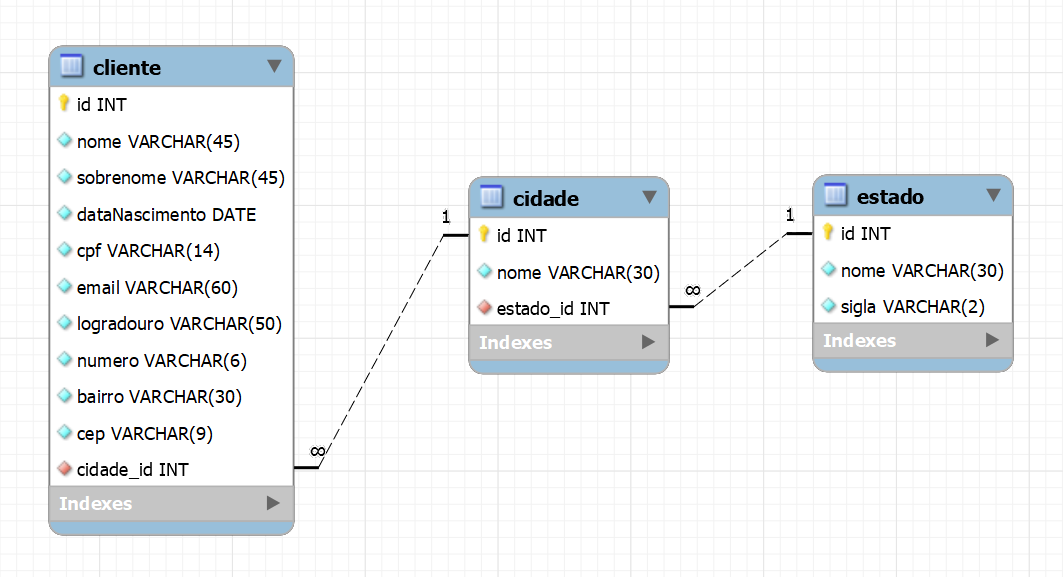
\includegraphics[scale=0.5]{imagens/cap05ModeloFisico}
    \\\textbf{Fonte:} Elaborada pelo autor
    \label{fig:cap05ModeloFisico}
\end{figure}
\FloatBarrier

Vamos agora implementar o banco de dados. No MySQL Workbench, crie uma nova base de dados com o nome de ``cadastro\_clientes'' como feito na Seção 4.2. Com a base criada, selecione-a no ``Object Browser'' e copie o código da Listagem~\thechapter.\ref{listagem:projetos/capitulo05/banco/estado.sql} no editor (Scratch) e execute o script.

\sqlCode{Script SQL para criação da tabela ``estado''}{projetos/capitulo05/banco/estado.sql}

Faça o mesmo processo para a Listagem~\thechapter.\ref{listagem:projetos/capitulo05/banco/cidade.sql} e para a Listagem~\thechapter.\ref{listagem:projetos/capitulo05/banco/cliente.sql}.

\sqlCode{Script SQL para criação da tabela ``cidade''}{projetos/capitulo05/banco/cidade.sql}

\sqlCode{Script SQL para criação da tabela ``cliente''}{projetos/capitulo05/banco/cliente.sql}

Ao fazer esses três passos, temos nossas três tabelas criadas dentro da base de dados. Clique com o botão direito no ``Object Browser'' e escolhe ``Refresh All''. Expanda o banco ``cadastro\_clientes'' e então expanda a pasta ``Tables''. Lá dentro estarão as três tabelas criadas. Muito bem, terminamos a implementação do banco. Vamos agora criar um diagrama de classes para representar cada uma das nossas entidades, que serão mapeamentos das nossas tabelas no mundo orientado a objetos.



\section{Criando o Diagrama de Classes}

Para criar nosso diagrama de classes UML, vamos usar a ferramenta astah* UML (o antigo JUDE UML) que pode ser obtida através do endereço http://astah.change-vision.com/. Usaremos a versão ``Community'' que é gratuita. Como já disse cada tabela do nosso banco de dados vai ter uma representação na nossa aplicação. Essa representação, como você já sabe, é criada usando classes. No diagrama de classes da Figura~\ref{fig:cap05DiagramaClasses}, você pode ver as três classes que representam nossas entidades. Note que cada classe contém uma série de atributos privados que representam as colunas da tabela e que o acesso a esses atributos é feito usando os métodos get e set correspondentes (omitidos no diagrama). 


\FloatBarrier
\begin{figure}[!htbp]
    \centering
    \caption{Diagrama de classes das entidades}
    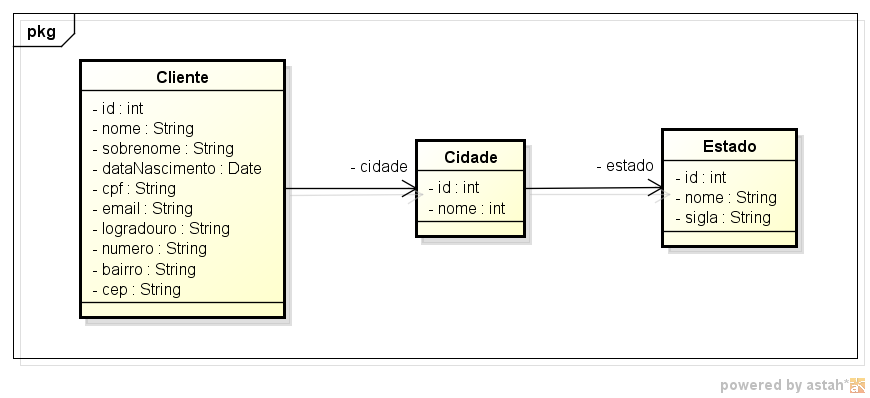
\includegraphics[scale=0.5]{imagens/cap05DiagramaClasses}
    \\\textbf{Fonte:} Elaborada pelo autor
    \label{fig:cap05DiagramaClasses}
\end{figure}
\FloatBarrier




Outro detalhe é que criei apenas o diagrama das classes que são as entidades do sistema, não me preocupando com as outras classes que nosso sistema conterá. Novamente, como no exemplo do nosso banco de dados, em um sistema de verdade, normalmente são desenvolvidos diagramas de classes muito mais completos e complexos, bem como outros tipos de diagramas UML que forem necessários. Com tudo isso pronto, podemos partir para o desenvolvimento do sistema propriamente dito!



\section{Construindo o Sistema}

Nossa primeira tarefa será criar o projeto no NetBeans. Para isso, abra o NetBeans e crie um novo projeto do tipo Java Web com o nome de ``CadastroClientes'' (sem as aspas). Marque a opção para usar uma pasta dedicada para armazenar as bibliotecas. Com o projeto criado, acesse suas propriedades e desmarque a opção ``Implantar ao salvar''. Nas bibliotecas, importe a ``JSTL 1.1'' e o ``MySQL JDBC Driver'' e após importar, adicione no projeto.
Em ``Pacotes de código-fonte'', crie o pacote ``cadastroclientes'' (sem as aspas) e os pacotes ``controladores'', ``dao'', ``entidades'', ``jdbc'' e ``testes'' dentro do pacote ``cadastroclientes''. Em ``Páginas Web'', crie os diretórios ``formularios'' (sem acento) e dentro deste, crie os diretórios ``cidades'', ``clientes'' e ``estados''. Veja na Figura 5.3 como deve ficar a estrutura do projeto.






Figura 5.3: Estrutura do projeto
 
Fonte: Print screen, NetBeans IDE 6.9.1

Com a estrutura configurada, vamos agora copiar algumas classes do projeto ``PadroesEmPatrica'' que criamos na aula anterior. Para isso abra esse projeto, se ainda não estiver aberto, no NetBeans. Expanda o pacote ``padroesempratica.jdbc'', clique com o botão direito no arquivo ``ConnectionFactory.java'' e escolha ``Copiar''. Volte ao projeto ``CadastroClientes'', clique com o botão direito no pacote ``cadastroclientes.jdbc'', escolha ``Colar'' e então ``Refatorar Copiar...''. Um diálogo será aberto. Clique no botão ``Refatorar''. O arquivo será copiado para o projeto e as alterações que forem necessárias fazer no arquivo, como mudar a cláusula ``package'', serão feitas pelo NetBeans. Faça o mesmo processo para o arquivo ``DAO.java'' contido no pacote ``pradoesempratica.dao'' do projeto ``PadroesEmPratica'', copiando-o no pacote ``cadastroclientes.dao'' do projeto ``CadastroClientes''. O NetBeans vai apontar um erro no arquivo depois da cópia. Para corrigir, abra o arquivo no editor e altere o ``import'' que está com problema. 
Outro detalhe é que precisamos mudar a URL da nossa fábrica de conexões para fazer com que as conexões criadas sejam relativas à base de dados ``cadastro\_clientes''. Para isso, abra o arquivo ``ConnectionFactory.java'' do pacote ``cadastroclientes.jdbc'' e mude a URL de ``jdbc:mysql://localhost/testes\_padroes'' para ``jdbc:mysql://localhost/cadastro\_clientes''.
Agora vamos preparar toda a camada de persistência. No pacote ``cadastroclientes.entidades'', crie três classes: ``Estado'', ``Cidade'' e ``Cliente'' (sem as aspas). Nas três listagens a seguir estão listados os códigos-fonte das três classes. Note que estou omitindo os gets e os sets, mas isso não significa que eles não devam existir. Fica por sua conta criar os gets e sets ok? Não se esqueça de fazer isso!

Listagem 5.4: Entidade ``Estado''
 
Fonte: do autor
Listagem 5.5: Entidade ``Cidade''
 
Fonte: do autor








Listagem 5.6: Entidade ``Cliente''
 
Fonte: do autor
Com as entidades prontas, vamos criar os DAOs. No pacote ``cadastroclientes.dao'', crie três classes: ``EstadoDAO'', ``CidadeDAO'' e ``ClienteDAO''. O código-fonte de cada uma dessas classes é apresentado nas listagens a seguir. Atenção! As listagens foram divididas.











Listagem 5.7: Código da classe ``EstadoDAO'' (parte 1)
 
Fonte: do autor
Listagem 5.8: Código da classe ``EstadoDAO'' (parte 2)
 Fonte: do autor






Listagem 5.9: Código da classe ``EstadoDAO'' (parte 3)
 
Fonte: do autor











Listagem 5.10: Código da classe ``CidadeDAO'' (parte 1)
 
Fonte: do autor
Listagem 5.11: Código da classe ``CidadeDAO'' (parte 2)
 Fonte: do autor
Listagem 5.12: Código da classe ``CidadeDAO'' (parte 3)
 Fonte: do autor




Listagem 5.13: Código da classe ``ClienteDAO'' (parte 1)
 
Fonte: do autor
Listagem 5.14: Código da classe ``ClienteDAO'' (parte 2)
 
Fonte: do autor


Listagem 5.15: Código da classe ``ClienteDAO'' (parte 3)
 
Fonte: do autor
Listagem 5.16: Código da classe ``ClienteDAO'' (parte 4)
 
Fonte: do autor



Listagem 5.17: Código da classe ``ClienteDAO'' (parte 5)
 
Fonte: do autor
Quantos códigos hein? Copiou tudo? Crie algumas classes de teste no pacote ``cadastroclientes.teste'' e teste a persistência de cada entidade. Com isso, terminamos a parte da persistência do nosso projeto.
Agora nós vamos começar a implementar as visualizações e os controladores. Nossa aplicação terá três links no index.jsp, sendo que cada link levará a um determinado cadastro. Cada cadastro vai conter uma página principal onde todos os itens desse cadastro serão exibidos e onde poderão ser alterados, excluídos ou então poderemos cadastrar um novo item.
Vamos começar pelo cadastro de estados. Na pasta ``estados'' dentro da pasta ``formularios'', crie um arquivo JSP com o nome de ``listagem'' (sem as aspas). Nesse arquivo vão ser listados todos os estados, portanto precisamos obter esses estados de alguma forma. Você se lembra que nos nossos DAOs existe um método chamado listarTodos que retorna todos os registros de uma determinada tabela? Nós não vamos usar esse método diretamente no JSP, então vamos criar uma classe de serviços que vai instanciar o DAO, gerar a lista e fechar a conexão para nós. Nos pacotes de código-fonte, crie um novo pacote dentro do ``cadastroclientes'' chamado ``servicos'' (sem o ``ç''). Nesse pacote, crie uma classe chamada ``EstadoServices'' (sem as aspas). Essa classe vai ter apenas um método, chamado getTodos, que retornará uma lista de estados. Veja o código-fonte dela na Listagem 5.18.
Listagem 5.18: Código-fonte da classe EstadoServices
 
Fonte: do autor
Criamos essa classe para que ela encapsule todo o processo de obtenção da lista de estados. Note que é no método getTodos que o EstadoDAO vai ser instanciado e gerenciado.
Agora que temos a classe que vai obter a lista de estados para nós, além de gerenciar o DAO, nós podemos implementar o nosso arquivo de listagem de estados. Abra o arquivo ``/formulários/estados/listagem.jsp'' e copie o código da Listagem 5.19.























Listagem 5.19: Código-fonte do arquivo ``/formularios/estados/listagem.jsp''
 
Fonte: do autor
Vamos analisar o código. Na linha 18, usamos a EL ``\${pageContext.request.contextPath}'' que vai gerar o caminho completo dos recursos da aplicação. Nesta linha, criamos um link que aponta para o arquivo ``/formularios/estado/novo.jsp'' – que ainda não implementamos – e que será o formulário responsável em criar um novo estado. Este mesmo código é repetido na linha 46. Na linha 20, abrimos a tag de uma tabela e, até a linha 29, criamos seu cabeçalho. Na linha 32, usamos a tag jsp:useBean para instanciar um objeto do tipo EstadoServices, que contém o método que vamos usar para obter a lista de estados. Demos o nome de ``servicos'' para essa instância. Na linha 34, usamos um c:forEach para iterar sobre a lista retornada pelo método getTodos da instância ``servicos''. Note que a chamada do método getTodos é somente ``todos'', pois seguimos o padrão JavaBeans nas ELs como você deve se lembrar. Essa chamada é feita usando EL na propriedade ``items''. Na propriedade ``var'', damos o nome da variável que vai armazenar a instância atual durante a iteração, no caso, ``estado''. Entre as linhas 35 e 41 nós definimos o código que será gerado a cada iteração do c:forEach. As três primeiras colunas da tabela são fáceis de entender, entretanto a quarta e a quinta mudam um pouco. Na linha 39, a coluna é formada por um link que aponta para ``/processaEstados?acao=prepAlteracao\&id=\${estado.id}''. Note que estamos codificando na URL duas variáveis. A primeira, chamada ``acao'', vai informar para o Servlet que vai estar mapeado para /processaEstados o que queremos fazer, no caso, ``prepAlteracao'' (preparar alteração). A segunda variável, chamada ``id'' vai conter o id do estado daquela linha da tabela, ou seja, queremos alterar um estado que tem um determinado id. O mesmo acontece na linha 40, mudando a ação para ``prepExclusao'' (preparar exclusão). Sei que pode estar um pouco confuso, mas na hora que terminarmos todos os arquivos do cadastro de estados tudo isso vai ficar fácil de entender, não se preocupe.
Note que deixei a linha 11 por último. Nela usamos a tag link para referenciar um arquivo de folhas de estilos. Nos exemplos das aulas anteriores nós usamos estilos declarados dentro do arquivo JSP usando a tag style. A partir de agora iremos separar os estilos em arquivos e é por isso que foi usada a tag link para a pontar para ``/css/estilos.css''. Vamos criar esse arquivo? Na pasta ``Páginas Web'', crie um diretório chamado ``css'' (sem as aspas), clique com o botão direito sobre ele e escolha ``Novo''. Provavelmente o item que queremos não estará visível, então escolha ``Outro...''. Escolha ``Web'' na categoria e em ``Tipo de arquivos'' escolha ``Folha de estilos em cascata''. Clique em próximo e dê o nome de ``estilos'' ao arquivo. Copie o código da Listagem 5.20 neste arquivo.








Listagem 5.20: Arquivo de estilos da aplicação
 
Fonte: do autor
Execute o projeto e aponte o navegador para a página de listagem para ver como está ficando. Se você já tiver alguns estados cadastrados, vai ver que eles aparecerão na tabela. Vamos agora criar nosso formulário para criar estados. Na pasta ``/formularios/estados'', crie um arquivo JSP chamado ``novo'' (sem as aspas). O código-fonte do arquivo pode ser visto na Listagem 5.21.



Listagem 5.21: Arquivo ``/formularios/estados/novo.jsp''
 
Fonte: do autor
Salve o arquivo e veja se ele está sendo exibido corretamente no navegador. Acesse-o pelo link ``Novo Estado'' da página de listagem de estados. Vamos analisar o código. Na linha 10 referenciamos o nosso arquivo de estilos. Nas linhas 18 e 19 declaramos a tag do formulário. Note que a action está apontando para ``/processaEstados'' que será a URL que mapearemos o Servlet que tratará os estados. A novidade nesse formulário é o uso de um input do tipo hidden (escondido). Esses tipos de input são usados para guardar valores que o usuário do sistema não tem acesso diretamente. No nosso caso, esse input, que tem o nome de ``acao'' e valor ``criar'', vai indicar ao Servlet que queremos criar um novo estado. Nós precisamos tratar isso na implementação do nosso Servlet ok? Como já temos nossa página de listagem e o nosso formulário de criação de estados, está na hora de criarmos o Servlet que vai gerenciar isso. No pacote ``cadastroclientes.controladores'', crie um Servlet com o nome de ``EstadosServlet'' (sem as aspas) e configure o mapeamento dele para ``/processaEstados'' (sem as aspas).
A seguir, na Listagem 5.22 e na Listagem 5.23, é apresentado o código do método processRequest do Servlet EstadosServlet.




















Listagem 5.22: Código-fonte do método processRequest do Servlet ``EstadosServlet'' (parte 1)
 
Fonte: do autor





Listagem 5.23: Código-fonte do método processRequest do Servlet ``EstadosServlet'' (parte 2)
 
Fonte: do autor
Copie todo o código e execute o projeto. Acesse a listagem de estados e clique para criar um novo estado. Preencha o formulário e salve. O novo estado será salvo e a listagem aparecerá novamente. Como exercício, tente entender o que está acontecendo no Servlet. Todo o código apresentado já foi estudado nos exemplos anteriores. Perceba que foram tratadas todas as ações possíveis, mas ainda faltam dois arquivos JSP para implementarmos. O ``alterar.jsp'' e o ``excluir.jsp''. Vamos fazer isso? Crie um arquivo na pasta ``/formularios/estados'' com o nome de ``alterar'' (sem as aspas) e copie o código da Listagem 5.24.

























Listagem 5.24: Código do arquivo ``/formularios/estados/alterar.jsp''
 
Fonte: do autor
Note que não numerei as linhas dessa listagem, visto que as diferenças importantes em relação ao arquivo novo.jsp são poucas. O que foi alterado é o input hidden nomeado como ``acao'', que agora tem o valor ``alterar''. Foi criado outro input hidden para armazenar o id do estado que será alterado. Note que os valores dos campos são preenchidos usando o atributo ``estado'' que foi configurado no request dentro do Servlet, na seção do código que trata a ação ``prepAlteracao''.
O arquivo excluir.jsp é bem parecido, só que neste arquivo não precisamos ter campos de entrada para nome e sigla, pois não vamos alterar esses dados. O importante é o id, que novamente vai ser configurado em um campo escondido. Veja na Listagem 5.25 o código do arquivo ``/formularios/estados/excluir.jsp'' que você deve criar.




















Listagem 5.25: Código do arquivo ``/formularios/estados/excluir.jsp''
 
Fonte: do autor
Copiou tudo? Teste! Verifique se tudo está funcionando corretamente. Antes de partirmos para os outros cadastros, vamos alterar o index.jsp criando três links, um para cada listagem dos cadastros. O novo código do index.jsp pode ser visto na Listagem 5.26.

Listagem 5.26: Código-fonte do index.jsp
 
Fonte: do autor
Teste o index.jsp e veja que agora ele tem três links para cada um dos cadastros. O que falta agora para terminarmos nosso projeto é implementar todos os JSPs dos outros cadastros, bem como seus respectivos Servlets e classes de serviço. A seguir, vou listar cada um desses arquivos, agrupando-os por tipo de cadastro, sendo que só irei comentar as linhas que contenham código que ainda não utilizamos ou que precisem de alguma explicação. Não se esqueça de testar o projeto sempre que tiver implementado os arquivos necessários para o funcionamento de uma determinada funcionalidade. Outro detalhe é que algumas linhas de código de algumas listagens foram divididas em duas linhas (nas listagens anteriores eu usei uma flecha para indicar isso), então preste atenção nas linhas que iniciam logo na margem esquerda, pois elas fazem parte da linha anterior. Antes das listagens vou indicar qual arquivo que estamos implementando. Lembre-se de criá-lo antes! Vamos começar?
•	Arquivo ``cadastroclientes.servicos.CidadeServices.java'' (Listagem 5.27).



Listagem 5.27: Código-fonte da classe CidadeServices
 
Fonte: do autor
•	Arquivo ``/formularios/cidades/listagem.jsp'' (Listagem 5.28 e Listagem 5.29).




Listagem 5.28: Código-fonte do arquivo ``/formularios/cidades/listagem.jsp'' (parte 1)
 
Fonte: do autor











Listagem 5.29: Código-fonte do arquivo ``/formularios/cidades/listagem.jsp'' (parte 2)
 
Fonte: do autor
•	Arquivo ``/formularios/cidades/novo.jsp'' (Listagem 5.30).








Listagem 5.30: Arquivo ``/formularios/cidades/novo.jsp''
 
Fonte: do autor
Note que na linha 33 da Listagem 5.30 nós usamos o serviço getTodos() da classe EstadoServices para obter todos os estados cadastrados e com isso gerar as opções (tag option) do select (combo box). Note que o valor de cada option é o id associado a determinado estado, enquanto o que aparece ao usuário é a junção entre o nome e a sigla do mesmo estado. O id do estado selecionado será enviado ao Servlet por meio da variável ``idEstado'', configurada no atributo ``name'' da tag select.
•	Método processRequest do arquivo ``CidadesServlet.java'' contido no pacote ``cadastroclientes.controladores''. O padrão de URL do mapeamento desse Servlet deve ser configurado para ``/processaCidades'' (sem as aspas) (Listagem 5.31 e Listagem 5.32).



















Listagem 5.31: Código-fonte do método processRequest do Servlet ``CidadesServlet'' (parte 1)
 
Fonte: do autor



Listagem 5.32: Código-fonte do método processRequest do Servlet ``CidadesServlet'' (parte 2)
 
Fonte: do autor
•	Arquivo ``/formularios/cidades/alterar.jsp'' (Listagem 5.33 e Listagem 5.34).


Listagem 5.33: Código do arquivo ``/formularios/cidades/alterar.jsp'' (parte 1)
 
Fonte: do autor










Listagem 5.34: Código do arquivo ``/formularios/cidades/alterar.jsp'' (parte 2)
 
Fonte: do autor
Na Listagem 5.34 temos algo muito interessante. Note que construímos nosso select da mesma forma que fizemos na Listagem 5.30, entretanto precisamos saber qual é o estado que é usado na cidade que será alterada. Para isso, ao usarmos o c:forEach, nós comparamos o id de cada estado do cadastro com o id do estado associado à cidade que vai ser alterada. Caso os ids sejam iguais, isso quer dizer que é o estado usado na cidade, sendo assim, a tag option é gerada com um atributo a mais, o ``selected'', configurado como ``true''. Usando esse atributo, nós dizemos ao navegador que aquele determinado item deve ser selecionado por padrão.
•	Arquivo ``/formularios/cidades/excluir.jsp'' (Listagem 5.35).
Listagem 5.35: Código do arquivo ``/formularios/cidades/excluir.jsp''
 
Fonte: do autor
•	Arquivo ``cadastroclientes.servicos.ClienteServices.java'' (Listagem 5.36).
Listagem 5.36: Código-fonte da classe ClienteServices
 
Fonte: do autor
•	Arquivo ``/formularios/clientes/listagem.jsp'' (Listagem 5.37 e Listagem 5.38).



Listagem 5.37: Código-fonte do arquivo ``/formularios/clientes/listagem.jsp'' (parte 1)
 
Fonte: do autor









Listagem 5.38: Código-fonte do arquivo ``/formularios/clientes/listagem.jsp'' (parte 2)
 
Fonte: do autor
•	Arquivo ``/formularios/clientes/novo.jsp'' (Listagem 5.39, Listagem 5.40 e Listagem 5.41).









Listagem 5.39: Arquivo ``/formularios/clientes/novo.jsp'' (parte 1)
 
Fonte: do autor



Listagem 5.40: Arquivo ``/formularios/clientes/novo.jsp'' (parte 2)
 
Fonte: do autor



Listagem 5.41: Arquivo ``/formularios/clientes/novo.jsp'' (parte 3)
 
Fonte: do autor
•	Método processRequest do arquivo ``ClientesServlet.java'' contido no pacote ``cadastroclientes.controladores''. O padrão de URL do mapeamento desse Servlet deve ser configurado para ``/processaClientes'' (sem as aspas) (Listagem 5.42, Listagem 5.43, Listagem 5.44 e Listagem 5.45).














Listagem 5.42: Código-fonte do método processRequest do Servlet ``ClientesServlet'' (parte 1)
 Fonte: do autor






Listagem 5.43: Código-fonte do método processRequest do Servlet ``ClientesServlet'' (parte 2)
 
Fonte: do autor
Note que no início da Listagem 5.43 (linha 42), nós usamos a classe SimpleDateFormat para converter a data inserida pelo usuário no formulário para um objeto do tipo java.util.Date. Para fazer essa conversão, precisamos criar o SimpleDateFormat com o formato que estamos usando para a data, no caso ``dia dia / mês mês / ano ano ano ano'' (dia com dois dígitos, mês com dois dígitos e ano com quatro dígitos), que deve ser codificado como dd/MM/yyyy.  Para fazer a conversão, usamos o método ``parse'' de SimpleDateFormat, sendo que a String com a data que é passada para o método ``parse'' deve estar no formato especificado no construtor do SimpleDateFormat. Caso a String não esteja no formato correto, é lançada uma exceção do tipo ParseException que precisamos tratar.
Outro detalhe é que nossa classe Cliente não usa o tipo java.util.Date para representar datas, mas sim o tipo java.sql.Date. Sendo assim, após gerarmos a data com o método ``parse'', precisamos ainda criar um objeto do tipo java.sql.Date, que recebe como parâmetro o tempo em milissegundos (método getTime() de java.util.Date) da data desejada, ou seja, da data que foi criada a partir da String passada pelo usuário através do formulário.


















Listagem 5.44: Código-fonte do método processRequest do Servlet ``ClientesServlet'' (parte 3)
 
Fonte: do autor









Listagem 5.45: Código-fonte do método processRequest do Servlet ``ClientesServlet'' (parte 4)
 
Fonte: do autor
•	Arquivo ``/formularios/clientes/alterar.jsp'' (Listagem 5.46, Listagem 5.47 e Listagem 5.48).
















Listagem 5.46: Código do arquivo ``/formularios/clientes/alterar.jsp'' (parte 1)
 
Fonte: do autor







Listagem 5.47: Código do arquivo ``/formularios/clientes/alterar.jsp'' (parte 2)
 
Fonte: do autor
Para que possamos apresentar a data de nascimento (tipo java.sql.Date) do cliente que está passando pelo processo de edição em um formato específico, nós usamos a tag fmt:formatDate (linha 46 da Listagem 5.47), que faz parte da JSTL. Note que a TagLib que contém essa tag é declarada no início da Listagem 5.46 usando o prefixo ``fmt''. Na tag fmt:formatDate, usada na Listagem 5.47, usamos o atributo ``pattern'' (padrão) para configurarmos o formato da String que deve ser gerada a partir da data de nascimento do cliente. O atributo ``value'' é usado para indicar o objeto da data que faz parte do objeto ``cliente'' contido no ``requestScope'', ou seja, o objeto que queremos formatar. O atributo ``var'' é usado para indicar o nome da variável usada para armazenar o resultado da formatação, sendo que no caso, configuramos o nome da variável como ``data''. Por fim, o atributo ``scope'' é usado para definir o escopo que essa variável vai existir, no caso, cofiguramos para ``page'', ou seja, a variável só vai existir dentro dessa página. A seguir, como valor do input da data de nascimento, usamos a variável ``data'', obtida usando EL na forma \${data}.





















Listagem 5.48: Código do arquivo ``/formularios/clientes/alterar.jsp'' (parte 3)
 
Fonte: do autor
•	Arquivo ``/formularios/clientes/excluir.jsp'' (Listagem 5.49 e Listagem 5.50).

Listagem 5.49: Código do arquivo ``/formularios/clientes/excluir.jsp'' (parte 1)
 
Fonte: do autor
Veja que no final da Listagem 5.49 (linha 38) usamos novamente um formatador de datas (tag fmt:formatDate) para apresentar a data de nascimento do cliente. Note que desta vez o uso do formatador foi simplificado, visto que agora não precisamos inserir a data formatada dentro de um input como fizemos na Listagem 5.47. Quando queremos apenas exibir a data formatada, basta usarmos a tag fmt:formatDate com os atributos ``pattern'' e ``value'' configurados que a data formatada será gerada onde a tag foi usada.


Listagem 5.50: Código do arquivo ``/formularios/clientes/excluir.jsp'' (parte 2)
 
Fonte: do autor
Ufa! Quanta coisa! Copiou todos os arquivos? Testou tudo o que você fez? Que bom! Se tudo funcionou, parabéns! Caso tenha dado algum problema, verifique o que pode ter acontecido, principalmente comparando o código que você copiou com o código das listagens. Agora você é capaz de criar uma aplicação Web em Java que contenha cadastros. Muito legal não é mesmo? Com essa bagagem teórica e prática que tivemos nessa e nas aulas anteriores, nós seremos capazes de trabalhar no projeto que será proposto na próxima aula.


\section{Resumo}

Nesta aula construímos uma aplicação Web completa que mantém o cadastro de Clientes, Cidades e Estados. Durante o nosso aprendizado, nós usamos os padrões que aprendemos na Aula 4 para criar a arquitetura da nossa aplicação, dividindo as responsabilidades entre as classes, bem como usando as camadas propostas no padrão MVC, organizando assim o nosso projeto. 

\section{Exercícios}

1 – Estude todos os arquivos de código-fonte que foram apresentados nesta aula e, mentalmente, descreva cada uma das linhas desses arquivos.
2 – Na listagem de clientes, insira uma nova coluna na tabela para apresentar a data de nascimento de cada cliente. Use a tag fmt:formatDate para formatar a data no formato dd/MM/yyyy (dia com dois dígitos, mês com dois dígitos e ano com quatro dígitos). Não se esqueça de usar a diretiva ``<%@taglib ...%>'' para configurar a TagLib de formatadores da JSTL. 
3 – Um detalhe que passou sem ser tratado no nosso projeto é a validação dos campos dos cadastros. Por exemplo, imagine que uma data de nascimento errada foi fornecida pelo usuário do sistema no cadastro de clientes, ou então que foi inserida uma sigla com mais de dois caracteres no cadastro de estados. Se esses dados forem passados de forma errada ao banco de dados, ele gerará um erro e então nosso cadastro não vai funcionar corretamente. Como você resolveria esse problema? Tente criar um mecanismo de validação dos dados fornecidos pelo usuário no cadastro de estados. Caso algum campo não tenha as características necessárias (sigla com mais de dois caracteres, por exemplo), direcione o usuário para uma página de erro, onde deve ser apresentado ao usuário qual erro ocorreu. Nessa página deve existir um botão ``Voltar'', que levará o usuário de volta à listagem de estados.
4 – Crie um mecanismo de validação de dados para o cadastro de cidades, da mesma forma que você fez para o cadastro de estados.
5 – Crie um mecanismo de validação de dados para o cadastro de clientes, da mesma forma que você fez para o cadastro de estados.


\section{Projetos}
\chapter{Segundo Projeto - Sistema para Locação de DVDs}\label{cap:segundoProjeto}
\epigraph{``\textit{É longo o caminho que vai do projeto à coisa}''.}{Molière}

\lettrine[lines=4, lhang=0.1, lraise=0, loversize=0.2, findent=0.1em]{\textcolor{corAzulTema}{N}}{ESTE} Capítulo aplicaremos o conhecimento adquirido na construção de uma aplicação Web em Java na construção de um projeto totalmente funcional.


\section{Introdução}

Neta Capítulo será apresentada uma série de requisitos que devem ser usados para criar uma aplicação Web da mesma forma que fizemos no Capítulo 5. Tudo que será requisitado estará baseado no que já aprendemos, sendo assim, todas as funcionalidades requeridas poderão ser implementadas com recursos já vistos no Capítulo 5.


\section{Apresentação dos Requisitos}

Você foi contratado para criar um sistema para controle de cadastro de DVDs. Esse sistema irá manter apenas o cadastro de DVDs e não irá gerenciar a locação dos mesmos. Os dados que deverão ser mantidos para todos os DVDs são: título, ano de lançamento, ator principal, ator coadjuvante, data de lançamento, duração em minutos, gênero e classificação etária. Os dados dos atores, dos gêneros e das classificações etárias deverão ser mantidos através de cadastros específicos. Um ator deve ter um nome, um sobrenome e uma data de estreia (indica quando foi o primeiro filme do ator). Um gênero deve ter uma descrição. Uma classificação etária deve ter também apenas uma descrição. Cada um dos cadastros (DVD, ator, gênero e classificação etária), deve conter as funcionalidades de criar, alterar e excluir um determinado registro. A página principal da aplicação deve conter um link para cada tipo de cadastro.


\section{Desenvolvimento do Projeto}

O projeto Web que deverá ser criado deve ter o nome de ``LocacaoDVDs''. Configure o projeto para conter as bibliotecas internamente. O pacote de código-fonte base do projeto deve ter o nome de ``\texttt{locacaodvds}''. A estrutura do projeto deve ser igual à estrutura do projeto criado no Capítulo 5, sendo que, obviamente, o nome das classes e suas respectivas implementações serão diferentes do projeto daquele Capítulo. A base de dados com as tabelas das entidades obtidas a partir da análise dos requisitos na seção anterior deve ter o nome de ``\texttt{locacao\_dvds}''. Não se esqueça de que cada entidade deverá conter um identificador. As páginas da aplicação deverão ter sua aparência configurada usando uma folha de estilos, da mesma forma que fizemos no projeto do Capítulo 5. Tente personalizar os estilos, mudando as cores etc. Você está livre para usar imagens ou qualquer outro artifício que julgar interessante para mudar a aparência da sua aplicação.


\section{Resumo}

Neste Capítulo foi requisitado que você implementasse uma aplicação Web em Java para gerenciar o cadastro de DVDs de uma locadora, por isso, não teremos exercícios para serem realizados. 


\section{Projetos}

\begin{projetoSemArquivo}{}{}{}
    A partir de tudo o que foi estudado e aprendido durante todas as aulas, faça um sistema para o gerenciamento de um frigorífico. Tente criar um texto que descreva os requisitos do sistema e então execute cada passo do desenvolvimento como sugerido neste Capítulo.
\end{projetoSemArquivo}

\begin{projetoSemArquivo}{}{}{}
     A partir de tudo o que foi estudado e aprendido durante todas as aulas, faça um sistema para o gerenciamento de uma escola. Tente criar um texto que descreva os requisitos do sistema e então execute cada passo do desenvolvimento como sugerido neste Capítulo.
\end{projetoSemArquivo}

%\chapter{Implantação}
\epigraph{``\textit{texto}''.}{autor}

\lettrine[lines=4, lhang=0.1, lraise=0, loversize=0.2, findent=0.1em]{\textcolor{corAzulTema}{N}}{ESTE} aaa.

\section{Introdução}

\section{Ferramentas}

%\chapter{JavaScript}\label{cap:javaScript}
\epigraph{``\textit{texto}''.}{autor}

\lettrine[lines=4, lhang=0.1, lraise=0, loversize=0.2, findent=0.1em]{\textcolor{corAzulTema}{N}}{ESTE} aaa.

\section{Introdução}

\section{Construções da Linguagem}

\section{JSON}

\section{Manipulação do DOM}

\section{jQuery}

\section{AJAX}

\section{Resumo}

\section{Exercícios}

\section{Projetos}

%\chapter{\textit{Frameworks} de Persistência}
\epigraph{``\textit{texto}''.}{autor}

\lettrine[lines=4, lhang=0.1, lraise=0, loversize=0.2, findent=0.1em]{\textcolor{corAzulTema}{N}}{ESTE} aaa.

\section{Introdução}

\section{Hibernate}

\section{JPA}

\section{Resumo}

\section{Exercícios}

\section{Projetos}

%\chapter{\textit{Frameworks} MVC}\label{cap:frameworksMVC}
\epigraph{``\textit{Não extingua sua inspiração e sua imaginação; não se torne o escravo do seu modelo}''.}{Vincent van Gogh}

\lettrine[lines=4, lhang=0.1, lraise=0, loversize=0.2, findent=0.1em]{\textcolor{corAzulTema}{N}}{ESTE} Capítulo serão tratados os conceitos básicos dos principais \textit{frameworks} para construção de aplicações Web em Java.

\section{Introdução}

\section{Spring Boot}

\section{Spring MVC}

\section{Integrações}

\section{Resumo}

\section{Exercícios}

\section{Projetos}

%\chapter{\textit{Frameworks} de \textit{Front End}}\label{cap:frameworksFront}
\epigraph{``\textit{A beleza interessa nos primeiros quinze dias; e morre, em seguida, num insuportável tédio visual}''.}{Nelson Rodrigues}

\lettrine[lines=4, lhang=0.1, lraise=0, loversize=0.2, findent=0.1em]{\textcolor{corAzulTema}{N}}{ESTE} Capítulo serão tratados os conceitos básicos dos principais \textit{frameworks} da camada de visualização que podem ser aplicados para construção de aplicações Web em Java.

\section{Introdução}

\section{Bootstrap}

\section{jQuery UI}

\section{AngularJS}

\section{Resumo}

\section{Exercícios}

\section{Projetos}

%\chapter{Tópicos Variados}\label{cap:topicosVariados}
\epigraph{``\textit{Há uma exuberância na bondade que parece ser maldade}''.}{Friedrich Nietzsche}

\lettrine[lines=4, lhang=0.1, lraise=0, loversize=0.2, findent=0.1em]{\textcolor{corAzulTema}{N}}{ESTE} Capítulo trateremos diversos temas pertinentes ao desenvolvimento de aplicações Web.

\vfill

\section{Introdução}

\section{\textit{Autenticação}}

\section{\textit{Gerenciamento de Sessões}}

\section{\textit{WebSockets}}

\section{\textit{WebStorage}}

\section{\textit{Node.js}}

\subsection{React}

\section{Resumo}

\section{Exercícios}

\section{Projetos}



\backmatter

\bibliography{referencias}


\end{document}
